%%%%%%%%%%%%%%%%%%%%%%%%%%%%%%%%%%%%%%%%%%%%%%%%%%%%%%%%%%%%%%%%%%%%%%%%%%%%%%%%%%%%%%%%%%
% Modelo LaTex para TCC e PIM do Programa de Graduação nas áreas de Computação da USCS % 
%         NÃO MODIFICAR ESSA PARTE, SOMENTE A PARTIR DE "INICIO DO DOCUMENTO"            %
%%%%%%%%%%%%%%%%%%%%%%%%%%%%%%%%%%%%%%%%%%%%%%%%%%%%%%%%%%%%%%%%%%%%%%%%%%%%%%%%%%%%%%%%%%

 \documentclass[
	% -- opções da classe memoir --
	12pt,					% tamanho da fonte
	openright,				% capítulos começam em pág ímpar (insere página vazia caso preciso)
	oneside,					% para impressão em somente um lado da folha.
	a4paper,					% tamanho do papel. 
	% -- opções da classe abntex2 --
	%chapter=TITLE,			% títulos de capítulos convertidos em letras maiúsculas
	%section=TITLE,			% títulos de seções convertidos em letras maiúsculas
	%subsection=TITLE,		% títulos de subseções convertidos em letras maiúsculas
	%subsubsection=TITLE,	% títulos de subsubseções convertidos em letras maiúsculas
	% -- opções do pacote babel --
	english,					% idioma adicional para hifenização
	%french,					% idioma adicional para hifenização
	%spanish,				% idioma adicional para hifenização
	portuguese					% o último idioma é o principal do documento
	]{abntex2}

% ----------------------
% Pacotes OBRIGATÓRIOS
% ----------------------
\usepackage{times}				% Usa a fonte Times New Roman
\usepackage[scaled]{helvet} % usa a fonte arial
\renewcommand\familydefault{\sfdefault} % mantém a fonte como padrão do documento
\usepackage[T1]{fontenc}		% Selecao de codigos de fonte.
\usepackage[utf8]{inputenc}		% Codificacao do documento (conversão automática dos acentos)
\usepackage{lastpage}			% Usado pela Ficha catalográfica
\usepackage{indentfirst}		% Indenta o primeiro parágrafo de cada seção.
\usepackage{color}				% Controle das cores
\usepackage{graphicx}			% Inclusão de gráficos
\usepackage{microtype} 			% Melhorias de justificação
\hypersetup{
    colorlinks=true,
    linkcolor=black,  % Changes internal links (like \ref) to black
    citecolor=black,  % Changes citations (like \cite) to black
    urlcolor=blue     % Changes URL links to blue
}
\pdfstringdefDisableCommands{\let\uppercase\relax}
\usepackage[lmargin=3cm,tmargin=3cm,rmargin=2cm,bmargin=2cm]{geometry} %Formato de margem nas normas ABNT
\setsecheadstyle{\bfseries \large}
% ---------------------
		
% ---------------------
% Pacotes ADICIONAIS
% ---------------------
\usepackage{lipsum}						% Geração de dummy text
\usepackage{amsmath,amssymb,mathrsfs}	% Comandos matemáticos avançados 
\usepackage{setspace}  					% Para permitir espaçamento simples, 1 1/2 e duplo
\usepackage{verbatim}					% Para poder usar o ambiente "comment"
\usepackage{tabularx} 					% Para poder ter tabelas com colunas de largura auto-ajustável
\usepackage{afterpage} 					% Para executar um comando depois do fim da página corrente
\usepackage{xurl} 						% Para formatar URLs (endereços da Web)
\usepackage{pdfpages}					% Para incluir documentos em PDF (anexos)
\setlength\afterchapskip{18pt}          % Ajusta o espaçamento entre o título do capitulo e o texto para 1,5
% \usepackage{titlesec}
\renewcommand{\ABNTEXchapterfontsize}{\bfseries\Large} % Define tamanho da fonte para capítulos, seções e sub seções.
\renewcommand{\ABNTEXsectionfontsize}{\bfseries\normalsize}
\renewcommand{\ABNTEXsubsectionfontsize}{\bfseries\normalsize}
\renewcommand{\ABNTEXsubsubsectionfontsize}{\bfseries\normalsize}
\usepackage[alf,bibjustif, abnt-etal-list=0,abnt-etal-cite=3]{abntex2cite}
% \citeoption{abnt-etal-cite=3}
% \usepackage{abntex2}
% ---------------------
% ---------------------
% Pacotes de CITAÇÕES
% ---------------------
%\usepackage[brazilian,hyperpageref]{backref}	% Paginas com as citações na bibl
%\usepackage[alf,bibjustif]{abntex2cite} % Citações padrão ABNT (alfa)
%\usepackage[num]{abntex2cite}				% Citações padrão ABNT (numericas)
% ---------------------

% O tamanho da identação do parágrafo é dado por:
\setlength{\parindent}{1.25cm}

% Controle do espaçamento entre um parágrafo e outro:
\setlength{\parskip}{0.2cm}  % tente também \onelineskip

% ---------------------
% Compila o indice
% ---------------------
\makeindex
% ---------------------




%%%%%%%%%%%%%%%%%%%%%%%%%%%%%%%%%%%%%%%%%%%%%%%%%%%%%%%%%%%%%%%%
%%  INICIO DO DOCUMENTO -- MODIFICAR A PARTIR DAQUI SOMENTE!! %%
%%%%%%%%%%%%%%%%%%%%%%%%%%%%%%%%%%%%%%%%%%%%%%%%%%%%%%%%%%%%%%%%
\input{extras/dados.tex}

% Quadros: o ambiente e a lista. A seção 4.8 só define o ambiente se ele faltar.
\providecommand{\quadroname}{Quadro}
\newfloat{quadro}{loq}{\quadroname}
\newlistof{listofquadros}{loq}{Lista de quadros}
\newlistentry{quadro}{loq}{0}
\renewcommand{\cftquadroname}{\quadroname\space}
\renewcommand*{\cftquadroaftersnum}{\hfill\textendash\hfill}

\begin{document}

% Configurações de CITAÇÕES para abntex2
\include{extras/conf_citacoes}

% Inclusão de dados para CAPA e FOLHA DE ROSTO (título, autor, orientador, etc.)
% Incluído na linha 94

% Inclui Configurações de aparência do PDF Final
\include{extras/conf_pdf}

% Retira espaço extra obsoleto entre as frases.
\frenchspacing


%%%%%%%%%%%%%%%%%%%%%%%%%%%%%%%%%%%%%%%%%%%%%%%%%%%%%%%%%%%%%%%%
%   ELEMENTOS PRÉ-TEXTUAIS (Capa, Resumo, Abstract, etc.)     %%
%%%%%%%%%%%%%%%%%%%%%%%%%%%%%%%%%%%%%%%%%%%%%%%%%%%%%%%%%%%%%%%%
\pretextual

% Capa
\include{1_pretextual/1_capa.tex}

%Contracapa
% ---
% Impressão da contracapa
% ---
  \begin{capa}%
    \begin{figure}[h!]%
        \centering%
        \includegraphics[scale=1]{figs/logo_uscs}%
      \end{figure}%
    \center   
    \ABNTEXchapterfont\bfseries\large{\imprimirinstituicao}
	%\vspace{1cm}
 
\vspace{2.5cm}

    \ABNTEXchapterfont\bfseries\large\imprimirtitulo 
    \vspace{2.5cm}
    
    \begin{flushright}
    
\begin{tabular}{@{}ll@{}}
    \hspace{.5cm} \textbf{Gabriel Correia Campari} & \textbf{RA: 8145921} \\ %% Nome dos autores do TCC
    \hspace{.5cm} \textbf{Gabriel Henrique Imolene Vieira} & \textbf{RA: 8154947} \\
    \hspace{.5cm} \textbf{Gustavo Almeida de Moura} & \textbf{RA: 8145857} \\
    \hspace{.5cm} \textbf{João Victor Maximiano Vieira} & \textbf{RA: 8151502} \\
    \hspace{.5cm} \textbf{Kaick Kenithi Nishiya} & \textbf{RA: 8143866} \\
    \hspace{.5cm} \textbf{Lucas Secanho do Prado} & \textbf{RA: 8164576}
\end{tabular}
	
    \end{flushright}
    \vfill
%
    \large\imprimirlocal \\ \large\imprimirdata

    \vspace*{1cm}
  \end{capa}
% ---

% Folha de rosto (o * indica que haverá a ficha bibliográfica)
%\imprimirfolhaderosto*
\include{1_pretextual/3_folhaderosto.tex}

% Imprimir Ficha catalográfica -- Deve ser impressa no verso da folha de rosto
% ---
% Ficha Catalográfica
% ---
% Isto é um exemplo de Ficha Catalográfica, ou ``Dados internacionais de
% catalogação-na-publicação''. Você pode utilizar este modelo como referência. 
% Porém, talvez a biblioteca lhe forneça um PDF
% com a ficha catalográfica definitiva após a defesa do trabalho. Quando estiver
% com o documento, salve-o como PDF no diretório do seu projeto e substitua todo
% o conteúdo de implementação deste arquivo pelo comando abaixo:
%
%\begin{fichacatalografica}
 %\center
    %\vspace*{\fill}	
    %{\includegraphics[scale=1]{figs/ficha_catalografica.pdf}}
 %\end{fichacatalografica}
 
% ---

\begin{fichacatalografica}
	\sffamily
	\vspace*{\fill}					% Posição vertical
	\begin{center}					% Minipage Centralizado
	\fbox{\begin{minipage}[c][8cm]{15.4cm}		% Largura
	\small
	
	\hspace{0.5cm} \imprimirtitulo { /} \imprimirautor. --
	\imprimirlocal, \imprimirdata.
	
	\hspace{0.5cm} \thelastpage f. : il. ; 30 cm.\\
	
	\hspace{0.5cm} \imprimirorientadorRotulo~\imprimirorientador\\
	
	\hspace{0.5cm}
	\parbox[t]{\dimexpr\linewidth-0.5cm\relax}{\imprimirtipotrabalho~--~\imprimirinstituicao,
	\imprimirdata.}\\
	
	\hspace{0.5cm}
		1. metabolômica. % Digitar as palavras-chave em ordem
		2. LC-MS.
        3. correção de deriva instrumental.
        4. controle de qualidade.
        5. quimiometria.
		I. Prof. Me. Raphael Lopes de Souza.
		II. Universidade Municipal de São Caetano do Sul.
		III. Ciência da Computação. % Especificar Curso
		IV. Título\\ 			
	\end{minipage}}
	\end{center}
\end{fichacatalografica}

% ; LC-MS; correção de deriva instrumental; controle de qualidade; quimiometria.

% Estrutura Organizacional USCS

% ---
% Definição do ambiente 'estrutura' para o modelo USCS
% ---
\newenvironment{estrutura}
 {
  \clearpage            % Começa em uma nova página
  \pagestyle{empty}     % Remove numeração de página nesta folha
 }
 {
  \clearpage            % Finaliza a página ao fechar o ambiente
 }
% ---

% ---
% Impressão da Folha de Estrutura da USCS
% ---
\begin{estrutura}

  \center
    \vspace*{\fill}	
    
    {\ABNTEXchapterfont\bfseries\ REITOR DA UNIVERSIDADE MUNICIPAL DE SÃO CAETANO DO SUL} \\
    \ABNTEXchapterfont\ {Prof. Dr. Leandro Campi Prearo} \\
    \vspace{0.5cm}
    {\ABNTEXchapterfont\bfseries\ PRÓ-REITOR DE GRADUAÇÃO} \\
    Prof. Me. Silton Marcell Romboli \\
    \vspace{0.5cm}
     {\ABNTEXchapterfont\bfseries\ GESTOR DOS CURSOS DE COMPUTAÇÃO} \\
    Prof. Me. Fabricio Ricardo Perrella

    \vspace*{1cm}
\end{estrutura}
% ---

% Página destinada a assinatura dos professores da Banca caso TCC seja aprovado
% ---
% Assinaturas
% ---
% Este é um exemplo de folha de aprovação, elemento obrigatório da NBR
% 14724/2011 (seção 4.2.1.3). Você pode utilizar este modelo até a aprovação
% do trabalho. Após isso, substitua todo o conteúdo deste arquivo por uma
% imagem da página assinada pela banca com o comando abaixo:
%
% \includepdf{folhadeaprovacao_final.pdf}
%
\begin{folhadeaprovacao}

  \begin{center}
  
{\ABNTEXchapterfont\large {\textbf{Universidade Municipal de São Caetano do Sul}}} \\
\vspace{1.5cm}
    %{\ABNTEXchapterfont\large\imprimirautor}
 \end{center}
\vspace{1cm}

    \begin{center}
      \ABNTEXchapterfont\bfseries\Large\imprimirtitulo
    \end{center}
    
 \vspace{1cm}
\begin{center} 
{\ABNTEXchapterfont {\imprimirpreambulo, avaliado pela banca examinadora composta por:}}
\end{center}
\vspace{1.5cm}
 % Isso na versao final do trabalho!!!       

   \ABNTEXchapterfont\assinatura{\textbf{\imprimirorientador} \\ Orientador}  % Alterar nome dos professores que irão compor a banca
   \ABNTEXchapterfont\assinatura{\textbf{Professor 1} \\ Universidade Municipal de São Caetano do Sul (USCS)}
   \ABNTEXchapterfont\assinatura{\textbf{Professor 2} \\ Universidade Municipal de São Caetano do Sul (USCS)}
   %\ABNTEXchapterfont\assinatura{\textbf{Professor 3} \\ Universidade Municipal de São Caetano do Sul (USCS)}
    \vfill
   \begin{center}
\vspace{0.5cm}
\imprimirlocal, 08 de dezembro de 2026 % Especificar data da defesa
    \vspace*{1cm}
  \end{center}
  
\end{folhadeaprovacao}
% ---

% Dedicatória
\include{1_pretextual/7_dedicatoria.tex}

% Agradecimentos
% ---
% Agradecimentos
% ---

\begin{agradecimentos}

Agradecemos ao Prof. Me. Ícaro de Paula Freitas, que orientou este trabalho em sua primeira metade, pela confiança no projeto e pelas orientações que deram a ele a sua forma inicial.

Agradecemos ao Prof. Me. Raphael Lopes de Souza, nosso orientador, pela disponibilidade, pela paciência e pelas orientações que conduziram este trabalho até a sua conclusão.

Agradecemos à Profa. Ma. Regina Albanese Pose, que participou das reuniões iniciais e, com o seu conhecimento em estatística e em tecnologia aplicada à saúde, nos guiou na direção de um projeto bem-sucedido.

Agradecemos de forma especial ao Prof. Dr. Álex Aparecido Rosini Silva e ao técnico de laboratório Marcos Eduardo Souza Abreu, do Laboratório de Metabolômica e Proteômica da USCS, vinculado ao INOVA-USCS, que se dispuseram a ser parte integrante deste projeto: apresentaram o problema, ajudaram a delimitar o escopo, esclareceram as nossas dúvidas sobre o assunto, recomendaram bibliografia, avaliaram a monografia e avaliaram o projeto final.

Agradecemos ao INOVA-USCS, centro de inovação da Universidade Municipal de São Caetano do Sul, por meio dos professores Dr. Carlos Eduardo Bognar e Dra. Sheila de Oliveira Garcia Mateos, que tornaram possível o contato com o Laboratório de Metabolômica e o acesso às suas necessidades.

Ao Prof. Me. Fabio Rezende de Souza, que demonstrou seu interesse no projeto e se prontificou a oferecer apoio caso precisássemos, nosso agradecimento pela generosidade e pela atenção.

Agradecemos também ao corpo docente da Universidade Municipal de São Caetano do Sul que cruzou o caminho das nossas turmas. O tempo e o esforço que esses professores dedicaram à nossa formação são o que nos permitiu chegar até aqui e realizar um projeto tão especial para nós.

\end{agradecimentos}

% ---



% Epígrafe
% \include{1_pretextual/9_epigrafe.tex}

% Resumo e Abstract
% ---
% RESUMOS
% ---

% RESUMO em português
\setlength{\absparsep}{18pt} % ajusta o espaçamento dos parágrafos do resumo
\begin{resumo}[Resumo]

 Dados de metabolômica não direcionada obtidos por cromatografia líquida acoplada à espectrometria de massas (LC-MS) chegam do processamento primário com erros sistemáticos do equipamento, e as etapas seguintes de refino — correção do sinal, filtragem, tratamento de valores ausentes, normalização, transformação e escalonamento — costumam ser feitas em ferramentas separadas, com escolhas manuais baseadas majoritariamente no conhecimento dos pesquisadores. Este trabalho apresenta o MetaRefino, aplicativo para Windows que assiste o pesquisador nesse refino a partir das matrizes exportadas pelo Progenesis QI: valida a entrada, diagnostica a forma da deriva instrumental, propõe as fronteiras de lote e o método de correção com justificativa, aplica as correções LOESS e SERRF ou mantém o sinal sem correção, executa o pré-processamento e as análises estatísticas univariadas e multivariadas, e exporta a matriz no formato do MetaboAnalyst. A escolha do corretor por um modelo de aprendizado de máquina não superou uma regra fixa e deu lugar, na interface, a uma medição sobre a própria matriz. A ferramenta foi avaliada com os dados de um único estudo do laboratório parceiro, com matrizes sintéticas derivadas deles e com a devolutiva escrita de seus usuários. O principal resultado veio da comparação entre réguas de qualidade: medida nos próprios controles de qualidade usados no ajuste, a correção LOESS fica à frente da ausência de correção nos quatro modos cromatográficos; medida fora da amostra, fica atrás dela em três. Conclui-se que a ferramenta integra e torna auditáveis as etapas do refino quimiométrico, com a decisão final mantida com o pesquisador; a generalização para outros estudos, laboratórios e equipamentos permanece por avaliar.
\vspace{\onelineskip}

 \noindent
 \textbf{Palavras-chave}: metabolômica; LC-MS; correção de deriva instrumental; controle de qualidade; quimiometria.
\end{resumo}

% ABSTRACT in english
\begin{resumo}[Abstract]
 \begin{otherlanguage*}{english}
   Untargeted metabolomics data acquired by liquid chromatography coupled to mass spectrometry (LC-MS) leave primary processing with systematic instrument errors, and the subsequent refinement steps --- signal correction, filtering, missing value treatment, normalization, transformation and scaling --- are usually carried out in separate tools, with manual choices based mainly on the researchers' knowledge. This work presents MetaRefino, a Windows application that assists researchers in this refinement, starting from the matrices exported by Progenesis QI: it validates the input, diagnoses the shape of the instrumental drift, proposes batch boundaries and a correction method with a justification, applies LOESS and SERRF correction or keeps the signal uncorrected, runs the preprocessing and the univariate and multivariate statistical analyses, and exports the matrix in the MetaboAnalyst format. Corrector selection by a machine learning model did not outperform a fixed rule and was replaced, in the interface, by a measurement on the matrix itself. The tool was evaluated on data from a single study of the partner laboratory, on synthetic matrices derived from them, and through written feedback from its users. The main result came from comparing quality yardsticks: measured on the same quality control samples used for fitting, LOESS correction outperforms no correction in all four chromatographic modes; measured out of sample, it falls behind in three. The tool integrates the chemometric refinement steps and makes them auditable, while the final decision remains with the researcher; generalization to other studies, laboratories and instruments remains to be evaluated.

   \vspace{\onelineskip}

   \noindent
   \textbf{Keywords}: metabolomics; LC-MS; instrumental drift correction; quality control; chemometrics.
 \end{otherlanguage*}
\end{resumo}

% Lista de ilustrações %%caso precise remover alguma das listas, inserir "%" na frente dos três comandos referente a mesma.%%
\pdfbookmark[0]{\listfigurename}{lof}
\listoffigures*                 
\cleardoublepage

% Lista de tabelas 
\pdfbookmark[0]{\listtablename}{lot}
\listoftables*
\cleardoublepage

% Lista de quadros
\pdfbookmark[0]{Lista de quadros}{loq}
\listofquadros*
\cleardoublepage

% Lista de abreviaturas e siglas
\begin{siglas}
  \item[API] Interface de programação de aplicações (Application Programming Interface)
  \item[CSV] Valores separados por vírgula (Comma-Separated Values)
  \item[FDR] Taxa de falsas descobertas (False Discovery Rate)
  \item[HILIC] Cromatografia de interação hidrofílica (Hydrophilic Interaction Liquid Chromatography)
  \item[IA] Inteligência Artificial
  \item[LC-MS] Cromatografia Líquida acoplada à Espectrometria de Massas
  \item[LOESS] Locally Estimated Scatterplot Smoothing
  \item[PCA] Análise de Componentes Principais
  \item[PLS-DA] Partial Least Squares Discriminant Analysis
  \item[PNG] Portable Network Graphics
  \item[POSIX] Portable Operating System Interface
  \item[PQN] Probabilistic Quotient Normalization
  \item[QC] Controle de qualidade
  \item[RF] Random Forest
  \item[RSD] Desvio padrão relativo
  \item[SERRF] Systematic Error Removal using Random Forest
  \item[SVM] Support Vector Machines
  \item[TIC] Corrente iônica total (Total Ion Current)
  \item[UTF-8] Unicode Transformation Format, 8 bits
  \item[VSN] Variance Stabilizing Normalization
\end{siglas}

% Lista de símbolos
\begin{simbolos}
\item[$\ll$] Muito menor que
\item[$\gg$] Muito maior que
\end{simbolos}

% Inserir o SUMÁRIO
\pdfbookmark[0]{\contentsname}{toc}
\tableofcontents*
\cleardoublepage


%%%%%%%%%%%%%%%%%%%%%%%%%%%%%%%%%%%%%%%%%%%%%%%%%%%%%%%%%%%
%%  ELEMENTOS TEXTUAIS (Capítulos/Contéudo do Trabalho)  %%
%%%%%%%%%%%%%%%%%%%%%%%%%%%%%%%%%%%%%%%%%%%%%%%%%%%%%%%%%%%
\textual %% Adiciona cabeçalho nas páginas, com numeração e título

\cleardoublepage % Finaliza todas as páginas pendentes e inicia uma nova página ímpar,
                 % garantindo que a numeração e o estilo sejam aplicados corretamente

\pagenumbering{arabic} % Define a numeração das páginas em algarismos arábicos (1, 2, 3...)

\setcounter{page}{16} % Define manualmente o número inicial da página.
                      % Ajustar conforme a quantidade de páginas pré-textuais do trabalho

% Define o estilo padrão das páginas
\makepagestyle{estiloTCC}

% Remove completamente cabeçalhos
\makeevenhead{estiloTCC}{}{}{}
\makeoddhead{estiloTCC}{}{}{}

% Adiciona o número da página no canto inferior direito
\makeevenfoot{estiloTCC}{}{}{\thepage}
\makeoddfoot{estiloTCC}{}{}{\thepage}

% Aplica o estilo ao documento inteiro
\pagestyle{estiloTCC}

% Faz os capítulos utilizarem o mesmo estilo
\aliaspagestyle{chapter}{estiloTCC}


% Inclui cada capitulo da Dissertação
% ----------------------------------------------------------
% Introdução 
% 
% ----------------------------------------------------------

\chapter[Introdução]{Introdução}

A metabolômica é uma das áreas mais recentes das ciências ômicas e tem como objetivo identificar e quantificar os metabólitos presentes em células, tecidos, fluidos biológicos e organismos. Os metabólitos são pequenas moléculas, geralmente com massa inferior a 1500 Da, e correspondem aos produtos finais das reações bioquímicas que acontecem no organismo. Enquanto a genômica analisa o DNA, a transcriptômica analisa o RNA e a proteômica analisa as proteínas, a metabolômica observa o resultado final desse fluxo de informação: o que de fato está sendo produzido pelas células em um determinado momento \cite{qiu2023small}. Por essa proximidade com o funcionamento real do organismo, alterações no perfil metabólico têm sido associadas a doenças, à resposta a tratamentos e a fatores nutricionais, ambientais e farmacológicos, o que tornou a metabolômica uma abordagem promissora para a descoberta de biomarcadores e para o avanço da medicina de precisão.
 
Entre as plataformas analíticas disponíveis, a cromatografia líquida acoplada à espectrometria de massas (LC-MS) é hoje uma das mais utilizadas em estudos de metabolômica não direcionada, abordagem que busca detectar o maior número possível de sinais na amostra, sem definir antecipadamente quais metabólitos analisar \cite{schrimpe2016untargeted}. A técnica funciona em duas etapas: primeiro, a cromatografia líquida separa os compostos da amostra com base em propriedades físico-químicas, como polaridade e carga; depois, o espectrômetro de massas detecta esses compostos e fornece informações como massa acurada, padrão isotópico e fragmentação molecular. Cada sinal detectado é descrito por três parâmetros (tempo de retenção, razão massa/carga (\textit{m/z}) e intensidade) e é chamado de \textit{feature} metabolômica, unidade básica das matrizes de dados que serão analisadas nas etapas seguintes \cite{chen2022guide}.
 
Apesar do grande potencial da LC-MS, os dados gerados por essa técnica não são simples de analisar. Os arquivos brutos contêm milhares de sinais, que precisam ser organizados em uma matriz estruturada por meio de etapas como alinhamento cromatográfico, detecção de picos e agrupamento de adutos, fragmentos e isótopos. Para essa etapa inicial, é comum o uso de softwares comerciais como o Progenesis QI, da Waters/Nonlinear Dynamics. Mesmo depois desse processamento primário, porém, a matriz resultante ainda pode apresentar variações técnicas entre amostras, sinais pouco reprodutíveis, redundâncias analíticas e falsos positivos causados por ruído do equipamento ou contaminação ambiental \cite{schiffman2019filtering}.
 
Por causa dessas inconsistências, antes de qualquer análise estatística é necessário realizar etapas adicionais de pré-processamento, como a avaliação da qualidade dos dados a partir de amostras de controle de qualidade (QCs), a filtragem de \textit{features} com alto desvio padrão relativo (RSD), o tratamento dos valores ausentes, a normalização entre amostras e a transformação e o escalonamento das intensidades. Para cada uma dessas etapas existem diferentes métodos disponíveis, e a escolha entre eles não é trivial. Cada decisão pode influenciar diretamente quais metabólitos aparecem como mais relevantes no resultado final, fazendo com que uma mesma matriz, processada de maneiras diferentes, possa levar a conclusões distintas \cite{vandenberg2006centering}. A complexidade aumenta ainda mais na análise estatística subsequente, dado que os dados metabolômicos têm alta dimensionalidade (com número de variáveis muito maior do que o número de amostras) e exigem métodos multivariados específicos, como PCA, PLS-DA e Random Forest \cite{worley2013multivariate}.
 
Outro problema comum na metabolômica é a fragmentação do fluxo de trabalho: cada etapa da análise costuma ser feita em um software diferente, como Progenesis QI, XCMS, MetaboAnalyst, SIMCA, R ou Python, o que aumenta o risco de erros, dificulta a padronização dos procedimentos e faz com que o resultado dependa muito da experiência individual do pesquisador \cite{weber2017computational}. Diante desse cenário, o uso de inteligência artificial (IA) e de aprendizado de máquina vem se mostrando uma alternativa interessante para apoiar o pesquisador nas decisões metodológicas que envolvem muitas variáveis técnicas e biológicas ao mesmo tempo. Quando essas técnicas são reunidas em um único ambiente de trabalho, é possível reduzir a fragmentação atual e tornar as decisões analíticas mais transparentes, padronizadas e reprodutíveis \cite{sen2021deep}.
 
É nesse contexto que se insere o presente trabalho, que propõe o desenvolvimento de uma plataforma para assistir no refino quimiométrico de matrizes de dados de LC-MS. A ferramenta proposta recebe como entrada as matrizes semiprocessadas geradas em softwares como o Progenesis QI e conduz, de forma assistida, etapas como filtragem por RSD, tratamento de valores ausentes, normalização, transformação, escalonamento e análise estatística.

\section{Objetivos}

\subsection{Objetivo Geral}

Desenvolver uma plataforma para o refino quimiométrico assistido de matrizes semiprocessadas de dados de metabolômica por cromatografia líquida acoplada à espectrometria de massas (LC-MS).

\subsection{Objetivos Específicos}

\subsubsection{Sistematizar as etapas de pré-processamento de dados metabolômicos não direcionados}
 
Identificar e organizar as principais etapas do refino quimiométrico (filtragem por desvio padrão relativo (RSD), tratamento de valores ausentes, normalização, transformação e escalonamento), que são determinantes para a interpretação biológica dos resultados em metabolômica \cite{vandenberg2006centering}.



\subsubsection{Estruturar um fluxo de trabalho assistido a partir das matrizes exportadas pelo Progenesis QI}
 
Desenvolver um pipeline integrado que receba as matrizes semiprocessadas geradas pelo Progenesis QI e conduza, de forma assistida, as etapas seguintes do refino quimiométrico, evitando a necessidade de alternar entre várias ferramentas distintas durante a análise.
 

\subsubsection{Incorporar algoritmos como sistema de apoio à decisão metodológica}
 
Integrar algoritmos determinísticos e de aprendizado de máquina capazes de orientar, a partir das características dos dados de entrada, a escolha dos métodos mais adequados de pré-processamento, normalização e análise estatística \cite{galal2022applications}.


\subsubsection{Implementar funcionalidades de análise estatística univariada e multivariada com critérios de validação}
 
Disponibilizar testes estatísticos univariados, com correção para múltiplas comparações via FDR, e métodos multivariados como PCA, PLS-DA e Random Forest, acompanhados de estratégias de validação cruzada e testes de permutação para reduzir o risco de sobreajuste \cite{worley2013multivariate}.

\subsubsection{Avaliar o desempenho da plataforma em dados reais e sintéticos}
 
Validar a ferramenta aplicando-a aos dados de metabolômica não direcionada do laboratório parceiro e a matrizes sintéticas com defeito conhecido, comparando os resultados com os do pipeline em R usado anteriormente pelo laboratório e avaliando a consistência das decisões metodológicas sugeridas pelo sistema.

\section{Justificativa}
 
A análise de dados metabolômicos não direcionados por LC-MS envolve diversos desafios técnicos, estatísticos e de interpretação. Mesmo depois de passar por um processamento inicial em softwares como o Progenesis QI, as matrizes resultantes ainda contêm variações técnicas, valores ausentes, sinais pouco reprodutíveis, redundâncias analíticas e possíveis falsos positivos. Por isso, são necessárias etapas adicionais de refino quimiométrico antes que qualquer análise estatística possa ser feita de forma confiável \cite{mahieu2017systems}. Essas etapas, no entanto, costumam ser realizadas em ferramentas separadas e frequentemente exigem conhecimentos avançados em estatística e programação. Isso fragmenta o fluxo de trabalho, prejudica a reprodutibilidade dos estudos e faz com que o resultado dependa fortemente da experiência individual do pesquisador \cite{weber2017computational}.
 
Além disso, a escolha entre os diferentes métodos de filtragem, imputação, normalização, transformação, escalonamento e análise estatística não é trivial. Como cada decisão pode levar a resultados diferentes a partir de uma mesma matriz, é fundamental contar com critérios sistemáticos, justificados e reprodutíveis \cite{diguida2016non}. Nesse cenário, ferramentas baseadas em algoritmos de auxílio à decisão, capazes de processar grandes volumes de dados, reconhecer padrões e auxiliar em decisões metodológicas, surgem como uma alternativa interessante para tornar o fluxo de análise metabolômica mais acessível, transparente e padronizado \cite{sen2021deep}.
 
Assim, desenvolver uma plataforma integrada para o refino quimiométrico assistido de dados de LC-MS pode contribuir tanto para o avanço metodológico da área quanto para tornar essas análises mais acessíveis, beneficiando pesquisadores com diferentes níveis de experiência em estatística e computação.

\section{Delimitação do estudo}

Este trabalho se limita ao desenvolvimento de uma plataforma computacional baseada em algoritmos de auxílio à decisão, voltada ao refino quimiométrico assistido de matrizes de dados gerados por cromatografia líquida acoplada à espectrometria de massas (LC-MS), no contexto de estudos de metabolômica não direcionada. Outras técnicas analíticas, como ressonância magnética nuclear (NMR), cromatografia gasosa acoplada à espectrometria de massas (GC-MS) e eletroforese capilar acoplada à espectrometria de massas (CE-MS), bem como estudos de metabolômica direcionada, não fazem parte do escopo deste trabalho.

A ferramenta atua em um estágio intermediário do fluxo de análise metabolômica, posicionada entre o processamento primário, feito pelo Progenesis QI, e as etapas finais de interpretação biológica. Sua entrada corresponde às matrizes semiprocessadas exportadas pelo Progenesis QI, normalmente em formato CSV, que contêm a caracterização das amostras (com a definição dos grupos experimentais) e uma planilha estruturada de \textit{features} identificadas por tempo de retenção, razão massa/carga (\textit{m/z}) e intensidade. Estão fora do escopo, portanto, todas as etapas anteriores a essa exportação, como o desenho experimental, a coleta e o preparo das amostras, a aquisição dos dados pelo espectrômetro de massas, a conversão dos arquivos brutos (\textit{raw}) e o alinhamento cromatográfico inicial.

Funcionalmente, a plataforma contempla a avaliação da qualidade analítica da matriz, a filtragem por desvio padrão relativo (RSD), o tratamento de valores ausentes, a normalização, a transformação, o escalonamento e as análises estatísticas univariadas e multivariadas. O foco está nas operações de caráter geral do refino de metabolômica não direcionada por LC-MS, que não dependem de um estudo específico. A validação, porém, é feita com os dados de um único estudo do laboratório parceiro, e com matrizes sintéticas derivadas deles; a generalização para outros estudos, laboratórios e equipamentos não foi avaliada e fica como trabalho futuro. Customizações para projetos individuais e a aplicação clínica direta em pacientes também ficam fora do escopo deste trabalho.
% ----------------------------------------------------------
% Revisão da Literatura
% 
% ----------------------------------------------------------


\chapter[Referencial Teórico]{Referencial Teórico}

{\section{\textbf{A Metabolômica}}}

A metabolômica consiste no estudo sistemático das ``impressões digitais'' químicas únicas deixadas por processos celulares, especificamente os perfis de metabólitos de moléculas pequenas (geralmente <1500 Da) presentes em células, tecidos e fluidos biológicos \cite{LILAND2011827,picone2026integrating}. Considerada o nível final da hierarquia das ciências ômicas, vindo após a genômica, transcriptômica e proteômica, ela fornece um instantâneo direto do estado fisiológico e patológico em tempo real, servindo como o elo mais próximo entre o genótipo e o fenótipo \cite{picone2026integrating,LILAND2011827,anwardeen2023statistical}. Essa abordagem é amplamente utilizada em aplicações como descoberta de biomarcadores, toxicologia, nutrição, medicina de precisão, agricultura e biologia de sistemas.

Com o avanço de tecnologias analíticas, tornou-se possível quantificar simultaneamente centenas ou milhares de metabólitos \cite{li2016performance}. As duas plataformas principais são a Espectrometria de Massas (MS) e a Ressonância Magnética Nuclear (NMR) \cite{anwardeen2023statistical}. A espectroscopia de NMR é uma técnica não destrutiva, altamente reprodutível e que exige preparação mínima de amostras, embora possua sensibilidade limitada que pode mascarar compostos em baixas concentrações \cite{mayonu2026evaluation}. Já a MS, frequentemente acoplada a técnicas de separação como cromatografia líquida (LC-MS) ou gasosa (GC-MS), oferece elevada sensibilidade e seletividade, permitindo a detecção de uma vasta gama de metabólitos polares, apolares ou voláteis. Essas tecnologias são essenciais para monitorar intervenções terapêuticas, estudos de microbioma e alterações em vias metabólicas associadas a diferentes estados biológicos \cite{pang2024metaboanalyst}.

O processo de geração de dados segue um fluxo de trabalho rigoroso que começa com o design experimental, fundamental para minimizar vieses e variações aleatórias por meio da randomização. Após a coleta e preparação de amostras, a aquisição de dados brutos gera sinais complexos (espectros ou cromatogramas) que precisam de pré-processamento \cite{LILAND2011827,anwardeen2023statistical}. Esta etapa crítica envolve a redução de ruído, correção de linha de base, detecção de picos (peak picking) e alinhamento de picos entre as amostras para converter sinais brutos em matrizes de intensidade interpretáveis \cite{sun2024pretreating}.

Entretanto, a geração desses volumes massivos de dados traz desafios significativos. Os conjuntos de dados metabolômicos apresentam alta dimensionalidade, em que o número de variáveis frequentemente excede o número de amostras ($N \ll P$), o que complica a análise estatística tradicional \cite{LILAND2011827,picone2026integrating}. Além disso, os dados são marcados pela esparsidade e presença de valores ausentes, causados por metabólitos abaixo do limite de detecção ou falhas técnicas de alinhamento \cite{li2016performance}. Outro fator complicador são os efeitos de lote (batch effects) e a deriva instrumental, que podem introduzir variações não biológicas e obscurecer o sinal biológico real \cite{li2016performance}.

É importante destacar que, mesmo após o pré-processamento, podem permanecer falsos positivos na matriz final — valores que não representam um metabólito verdadeiro, mas sim ruídos provenientes do equipamento ou do ambiente \cite{schiffman2019filtering}. Para mitigar esse risco, softwares especializados como o \textbf{Progenesis QI} incorporam rotinas adicionais de controle de qualidade, como a redução de dados sem perda de informação essencial, o mascaramento de regiões cromatográficas ruidosas, alertas automáticos de inconsistências de calibração e métricas visuais de alinhamento. Além disso, o software oferece funções de normalização robusta e ferramentas de estatística multivariada (como PCA e dendrogramas) que auxiliam na detecção de outliers e na validação visual dos sinais \cite{watersprogenesisguide}.

Devido a essa complexidade, o tratamento adequado das informações tornou-se uma das etapas mais desafiadoras e demoradas. O avanço das tecnologias aumentou a necessidade de ferramentas computacionais, softwares especializados e abordagens in silico capazes de auxiliar no processamento, anotação e visualização de dados multivariados. Assim, a integração de métodos de aprendizado de máquina e estatística avançada é indispensável para extrair padrões significativos e garantir a reprodutibilidade dos resultados em experimentos de larga escala.


\section{\textbf{Cromatografia Líquida acoplada à Espectrometria de Massas (LC-MS)}}

A cromatografia líquida acoplada à espectrometria de massas (LC-MS) consolidou-se como uma das principais técnicas analíticas utilizadas em metabolômica, especialmente em abordagens não direcionadas. Essa metodologia combina duas etapas fundamentais: a separação cromatográfica dos compostos presentes na amostra e a detecção desses compostos pelo espectrômetro de massas. A cromatografia líquida permite separar metabólitos de acordo com suas propriedades físico-químicas, como polaridade, hidrofobicidade, carga e interação com a coluna cromatográfica, o que é essencial para lidar com a elevada complexidade química de matrizes biológicas como plasma, soro, urina e extratos celulares \cite{chen2022guide}.

Após a separação, os compostos são direcionados ao espectrômetro de massas, onde são ionizados e analisados de acordo com sua razão massa/carga (m/z). Essa etapa fornece informações cruciais, como massa acurada, padrão isotópico e fragmentação molecular, permitindo a caracterização de metabólitos em baixas concentrações. Entretanto, durante o processo de ionização, um mesmo metabólito pode originar diferentes sinais relacionados, como adutos, fragmentos ou formas isotópicas, aumentando a complexidade da interpretação dos dados \cite{mahieu2017systems}.

Em equipamentos de alta resolução (LC-HRMS), é possível obter maior precisão na determinação da massa dos compostos, o que contribui para a anotação putativa dos metabólitos. No entanto, essa identificação deve ser interpretada com cautela, já que compostos distintos podem apresentar massas semelhantes, padrões de fragmentação parecidos ou formar adutos e isômeros relacionados. Em estudos de metabolômica não direcionada, cada sinal detectado é geralmente definido por três parâmetros principais: tempo de retenção, valor de m/z e intensidade. Esses sinais, chamados de features metabolômicas, são organizados em uma matriz de dados que servirá de base para etapas subsequentes de pré-processamento, normalização e análise estatística \cite{schrimpe2016untargeted}.

A LC-MS, portanto, oferece elevada sensibilidade e ampla cobertura metabólica, sendo capaz de detectar simultaneamente centenas ou milhares de metabólitos em uma única análise. Essa capacidade amplia significativamente o potencial de descoberta biológica, mas também aumenta os desafios computacionais e estatísticos envolvidos no tratamento, integração e interpretação das informações metabolômicas. Dessa forma, compreender as particularidades da LC-MS é essencial para a escolha adequada de técnicas de pré-processamento e controle de qualidade, garantindo maior confiabilidade e robustez nos resultados obtidos.


\section{\textbf{Características dos Dados Metabolômicos}}

Os dados provenientes de experimentos metabolômicos apresentam características específicas que tornam sua análise significativamente mais complexa quando comparada a conjuntos de dados tradicionais. Essas características estão relacionadas tanto à natureza biológica dos metabólitos quanto às limitações e particularidades das técnicas analíticas utilizadas durante a aquisição dos dados. A metabolômica envolve a caracterização em larga escala de metabólitos presentes em células, tecidos e organismos, utilizando principalmente plataformas analíticas como espectrometria de massas (MS) e ressonância magnética nuclear (NMR), cada uma com vantagens, limitações e requisitos específicos de processamento e interpretação dos dados \cite{chen2022guide}.

Em geral, os datasets metabolômicos são caracterizados por alta dimensionalidade, elevada variabilidade experimental, presença de ruídos, valores ausentes e grande heterogeneidade entre amostras. Além disso, os dados frequentemente apresentam distribuições assimétricas, relações não lineares entre variáveis, diferenças expressivas de escala entre variáveis e forte sensibilidade às condições experimentais. A identificação e quantificação dos metabólitos constituem tarefas complexas, que não podem ser completamente automatizadas e exigem cuidadoso processamento computacional e análise estatística para obtenção de informações confiáveis \cite{shahjaman2021rmisbeta}.

Outro aspecto relevante é que pequenas alterações instrumentais ou diferenças no preparo das amostras podem gerar impactos significativos nos sinais medidos, dificultando a separação entre variações técnicas e variações biológicas reais. Fatores como deriva instrumental, diferenças entre lotes experimentais, sensibilidade analítica e limitações das plataformas de aquisição podem introduzir padrões artificiais nos dados, tornando necessárias múltiplas etapas de pré-processamento, normalização e controle de qualidade antes da realização das análises estatísticas \cite{shahjaman2021rmisbeta}.

A complexidade desses dados também está diretamente relacionada à capacidade das tecnologias modernas, como espectrometria de massas (MS) e ressonância magnética nuclear (NMR), de detectar simultaneamente centenas ou milhares de metabólitos em uma única análise. Enquanto técnicas baseadas em MS oferecem alta sensibilidade e ampla cobertura metabólica, métodos baseados em NMR fornecem elevada reprodutibilidade e informações estruturais detalhadas dos compostos analisados. Embora essas tecnologias ampliem significativamente o potencial de descoberta biológica, também aumentam os desafios computacionais e estatísticos envolvidos no tratamento, integração e interpretação das informações metabolômicas \cite{NMR}.

Dessa forma, compreender as características dos dados metabolômicos é essencial para a escolha adequada de técnicas de pré-processamento, normalização e análise estatística, garantindo maior confiabilidade, robustez e interpretabilidade dos resultados obtidos.

\subsection{Alta Dimensionalidade}

Os dados metabolômicos são caracterizados por alta dimensionalidade, situação em que o número de variáveis analisadas frequentemente excede o número de amostras disponíveis, configurando o problema conhecido como $p \gg n$ \cite{gunawan2022data} . Nesse cenário, cada metabólito detectado pelas plataformas analíticas corresponde a uma variável do conjunto de dados, fazendo com que experimentos metabolômicos possam gerar centenas ou milhares de variáveis simultaneamente, mesmo em estudos com número limitado de amostras biológicas.

Essa característica está diretamente relacionada ao avanço de tecnologias analíticas modernas, como espectrometria de massas (MS) e ressonância magnética nuclear (NMR), capazes de detectar grande quantidade de compostos metabólicos em uma única análise \cite{NMR}. Como consequência, os datasets metabolômicos tornam-se altamente complexos, multidimensionais e frequentemente acompanhados de ruídos experimentais, variabilidade técnica e diferenças de escala entre variáveis.

Em geral, os dados metabolômicos são organizados em matrizes bidimensionais, nas quais as linhas representam as amostras biológicas e as colunas correspondem às intensidades dos metabólitos detectados. Essa estrutura matricial constitui a base para aplicação de métodos estatísticos, técnicas de redução de dimensionalidade e algoritmos de aprendizado de máquina \cite{gunawan2022data}.

No entanto, a elevada dimensionalidade dos dados impõe desafios significativos à análise estatística e computacional \cite{shahjaman2021rmisbeta}. Métodos estatísticos tradicionais podem apresentar baixo desempenho nesse contexto, especialmente devido ao aumento do risco de overfitting, à presença de correlações espúrias e à redução da capacidade de generalização dos modelos analíticos. Além disso, o aumento do número de variáveis dificulta a identificação de padrões relevantes, fenômeno frequentemente associado à chamada maldição da dimensionalidade \cite{gunawan2022data}.

Diante desse cenário, torna-se necessária a aplicação de técnicas específicas de pré-processamento e redução de dimensionalidade, como transformação de dados, seleção de variáveis e métodos como a Análise de Componentes Principais (PCA). Essas abordagens buscam reduzir a complexidade dos datasets metabolômicos, preservar informações biologicamente relevantes e aumentar a robustez das análises estatísticas e computacionais realizadas.

\subsection{Variabilidade Técnica e Biológica}

A metabolômica, com seus dados de alta dimensionalidade, enfrenta o desafio de separar os efeitos mistos que influenciam os níveis de metabólitos. Muitos métodos estatísticos e experimentais estruturados, como design de experimentos e modelagem multivariada, permitem decompor a variabilidade e associar cada metabólito às causas específicas. Esses métodos ajudam a identificar assinaturas fisiológicas ou patológicas de forma mais confiável \cite{boccard2023we}.

Para a identificação dessas assinaturas, são utilizadas estratégias como o uso de razões entre metabólitos (normalização interna e melhor interpretação de vias metabólicas), modelagem de redes metabólicas (conecta substratos e produtos para entender as rotas bioquímicas) e estudos longitudinais (acompanham alterações ao longo do tempo). Essas estratégias são essenciais para transformar a metabolômica de uma simples busca por biomarcadores em uma abordagem mecanística, capaz de explicar como os processos bioquímicos mantêm seu estado de condições internas relativamente constantes, a homeostase \cite{boccard2023we}.

Em alguns estudos de metabolômica em larga escala, a coleta e análise de amostras podem durar dias, meses ou até anos. Esse período pode gerar os efeitos de lote (batch effects), que são variações artificiais nos dados causadas por diferenças no estado do instrumento, condições ambientais ou operadores. Os batch effects podem mascarar as verdadeiras relações biológicas entre metabólitos \cite{guo2023concordance}. 

São utilizados alguns métodos tradicionais para a correção de lote (BEC), que empregam amostras de controle de qualidade (QC), mas estas podem se deteriorar em experimentos longos. Outra alternativa são padrões internos isotopicamente marcados, que não cobrem bem todo o metaboloma. Com isso, métodos data-driven (baseados apenas nos dados) surgiram como solução \cite{guo2023concordance}.

Um método proposto no artigo \cite{guo2023concordance} é o CordBat, que seleciona um lote de referência como baseline, constrói um modelo gráfico gaussiano com dados do lote de referência e dos demais, e ajusta os coeficientes dos outros lotes para que suas correlações entre metabólitos fiquem em concordância com as do lote de referência.

As plataformas analíticas modernas, como LC-MS, GC-MS, NMR e ion mobility, geram dados altamente complexos e multivariados. Métodos estatísticos tradicionais muitas vezes não conseguem lidar com essa complexidade. O machine learning surgiu como uma solução, permitindo reconhecimento de padrões, classificação, regressão e seleção de variáveis em dados de alta dimensionalidade \cite{picone2026integrating}. 

Diante disso, a complexidade e variabilidade dos dados são fatores preocupantes para a utilização dos métodos tradicionais atualmente, visto a alta demanda de tempo necessário para análise e tratamento desses dados. Tecnologias como o aprendizado de máquina (machine learning), subcampo da Inteligência Artificial (IA), surgem com o intuito de otimizar e dar suporte aos processos realizados por equipes biomédicas.


\subsection{Valores ausentes e zero}

 Na metabolômica baseada em espectrometria de massas, o tratamento dos dados é um passo crítico para garantir qualidade e confiabilidade das análises. Durante a aquisição e pré-processamento, etapas como compressão de dados, filtragem de ruído e correção de baseline são fundamentais para melhorar a consistência dos sinais. Em seguida, procedimentos como detecção de picos, deconvolução e alinhamento permitem identificar corretamente os metabólitos presentes.

Um dos maiores desafios está relacionado aos valores ausentes e zeros. Esses podem ocorrer por diferentes razões: limites de detecção do equipamento, supressão iônica, desalinhamento de picos ou inconsistências na aquisição do sinal. A ausência de valores pode ser classificada como missing completely at random (MCAR), missing at random (MAR) ou missing not at random (MNAR), sendo este último frequentemente associado a metabólitos em concentrações abaixo do limite de detecção. Já a esparsidade descreve a presença de grande proporção de valores nulos ou próximos de zero, comum em análises não direcionadas, onde nem todos os metabólitos são detectados em todas as amostras \cite{metabolomicsdatatreatment}.

Esses problemas afetam diretamente a inferência estatística e o desempenho dos modelos de machine learning, podendo introduzir vieses e distorcer a estrutura de variância dos dados. Para mitigar tais efeitos, são aplicadas estratégias de pré-processamento como imputação de dados (k-nearest neighbors, imputação múltipla ou métodos baseados em ML, como random forest imputation), além de filtragem de variáveis e transformações matemáticas. O uso adequado dessas técnicas é essencial para preservar a relevância biológica, melhorar a robustez dos modelos e garantir interpretações confiáveis \cite{metabolomicsdatatreatment}.


\section{\textbf{Pré-processamento de Dados em Metabolômica}}

Na metabolômica, existe uma etapa denominada pré-processamento de dados, na qual diferentes procedimentos são aplicados aos dados brutos antes da realização de análises estatísticas e computacionais. Essa fase possui elevada complexidade, devido à necessidade de transformar grandes volumes de dados em informações consistentes e adequadas para interpretação analítica. Os dados vêm, em geral, de duas plataformas de aquisição, a espectroscopia por ressonância magnética nuclear (RMN) e a espectrometria de massas (EM), esta frequentemente associada a métodos de separação cromatográfica, e cada uma exige procedimentos próprios de pré-processamento \cite{LILAND2011827}. 

Em experimentos metabolômicos, normalmente é gerada uma grande quantidade de dados, os quais raramente podem ser utilizados de forma direta, completa e isenta de interferências experimentais. Esses dados frequentemente apresentam ruídos, variações instrumentais, desalinhamentos e outros fatores que podem comprometer significativamente a qualidade e a confiabilidade das análises subsequentes. Dessa forma, torna-se necessária a aplicação de técnicas de pré-processamento e pré-tratamento para adequar os dados às etapas analíticas posteriores. Na literatura metabolômica, os termos “pré-processamento de dados” e “pré-tratamento de dados” são frequentemente utilizados de maneira inconsistente \cite{sun2024pretreating}. De forma mais específica, o pré-processamento está relacionado às etapas iniciais aplicadas aos dados brutos, incluindo filtragem de ruído, correção de linha de base, faseamento, alinhamento de picos e binning espectral \cite{sun2024pretreating}. Em alguns trabalhos, procedimentos como normalização e dimensionamento de variáveis também são incorporados a essa etapa. Já o pré-tratamento é geralmente associado às técnicas de transformação, centralização e escalonamento dos dados, podendo incluir também métodos de estimativa ou imputação de valores ausentes.

De maneira geral, todas as etapas realizadas antes da análise estatística podem ser consideradas parte do processo de pré-processamento e pré-tratamento de dados. Entre as ciências ômicas, a metabolômica não direcionada destaca-se na busca por biomarcadores em sistemas biológicos complexos, permitindo analisar a resposta de organismos, tecidos ou células a estímulos externos e relacionar condições experimentais a alterações fenotípicas de interesse. Sua principal vantagem consiste na capacidade de fornecer um “instantâneo metabólico” do sistema biológico analisado. Entretanto, um dos principais desafios dessa abordagem está relacionado ao processamento de grandes volumes de dados, exigindo métodos computacionais robustos e eficientes para tratamento e interpretação das informações obtidas \cite{schrimpe2016untargeted}. Nesse contexto, as etapas de pré-processamento e pré-tratamento possuem papel fundamental, pois buscam minimizar artefatos instrumentais e variabilidades biológicas irrelevantes, melhorar a relação sinal-ruído (SNR, do inglês Signal-to-Noise Ratio) e transformar os dados em perfis espectrais mais interpretáveis, reduzindo sua dimensionalidade e aumentando a confiabilidade das análises metabolômicas \cite{sun2024pretreating}.

\subsection{Etapas de pré-processamento}

As etapas de pré-processamento no Progenesis QI seguem um fluxo de trabalho integrado projetado para preparar os dados de LC-MS para análise quantitativa e identificação posterior. O processo inicia-se com a Importação de Dados, fase na qual o software realiza uma rotina de redução de dados e aplica a calibração de massa (lock mass) para garantir a integridade e precisão das medições \cite{watersprogenesisguide}. Durante essa carga inicial, é realizada uma revisão de controle de qualidade (QC) para alertar sobre possíveis erros, como polaridade incorreta ou arquivos convertidos indevidamente para o formato centroided. Também é possível utilizar máscaras para excluir áreas ruidosas do mapa de íons, geralmente no início ou fim da corrida, causadas pela regeneração da coluna \cite{watersprogenesisguide}.

Em seguida, o Alinhamento atua compensando variações nos tempos de retenção entre as diferentes corridas analíticas, assegurando que as mesmas características sejam comparadas de forma consistente em todo o conjunto de dados. Esse processo exige a escolha de uma ``corrida de referência'', que pode ser selecionada automaticamente pelo software através da análise de similaridade entre todas as amostras, ou manualmente pelo usuário \cite{watersprogenesisguide}. O software fornece métricas visuais de qualidade, utilizando cores que variam do verde ao vermelho para indicar a precisão do alinhamento em diferentes regiões do mapa de intensidade de íons \cite{watersprogenesisguide}.

A detecção propriamente dita ocorre na etapa de Peak Picking, na qual são estabelecidos parâmetros e limiares para localizar os picos dos íons dos compostos em todas as corridas alinhadas \cite{watersprogenesisguide}. O usuário pode ajustar a sensibilidade da detecção e definir janelas mínimas para a largura de pico cromatográfico \cite{watersprogenesisguide}. Uma funcionalidade importante permite que apenas corridas de alta qualidade contribuam para o padrão de detecção de picos, evitando que amostras ruidosas prejudiquem o mapeamento de características em todo o experimento \cite{watersprogenesisguide}.

Posteriormente, a Normalização ajusta as abundâncias para permitir comparações estatísticas justas entre as amostras. O sistema identifica automaticamente a corrida ``menos diferente'' para servir como referência de normalização \cite{watersprogenesisguide}. Embora o método padrão considere todos os compostos detectados, o software oferece flexibilidade para normalizar com base em padrões externos ou em um conjunto específico de compostos de referência (housekeeping). Na determinação do fator de normalização, compostos que se comportam como outliers são automaticamente ignorados pelo algoritmo \cite{watersprogenesisguide}.

Por fim, a Desconvolução agrupa automaticamente as diversas formas de adutos de um único composto, consolidando a quantificação precisa da molécula original a partir da sua massa neutra \cite{watersprogenesisguide}. O cálculo da massa neutra depende da detecção de pelo menos dois adutos diferentes para o mesmo composto. Esta fase permite uma revisão detalhada, na qual o analista pode adicionar ou remover manualmente adutos específicos caso seus perfis cromatográficos ou de espectro de massa não correspondam à maioria dos íons agrupados para aquele composto \cite{watersprogenesisguide}.

\subsection{O papel do Progenesis QI no Pré-processamento Primário }

No âmbito do pré-processamento de dados metabolômicos, o software Progenesis QI (proprietário da empresa estadunidense Waters) consolida-se como uma plataforma de referência para a extração e o tratamento primário de características analíticas \cite{watersprogenesisguide}. Suas funções mais relevantes concentram-se no pipeline inicial de processamento: o alinhamento cromatográfico para a correção de desvios nos tempos de retenção, a co-detecção de picos — que mitiga a ocorrência de dados ausentes através da integração do ruído de fundo — e a deconvolução espectral, responsável por agrupar fragmentos, adutos e isótopos em entidades moleculares únicas. Após a finalização desse processo de deconvolução e quantificação dos compostos, antecedendo qualquer tentativa de modelagem ou filtragem estatística multivariada no ambiente nativo do software, as informações semiprocessadas são exportadas, e o pré-processamento é completado na ferramenta proposta. Nesse ponto, a matriz de abundâncias biológicas encontra-se unificada em um formato estruturado, porém altamente suscetível a falsos positivos latentes e derivas instrumentais, configurando o cenário e o insumo ideais para que a ferramenta assuma o fluxo e inicie o refino quimiométrico assistido. 

\section{\textbf{Tratamento de Dados Metabolômicos}}

O tratamento de dados metabolômicos constitui uma etapa crítica para transformar sinais analíticos brutos em matrizes limpas e comparáveis, aptas para análises estatísticas e interpretações biológicas \cite{datanor,sun2024pretreating}. Esse processo é multifacetado e busca minimizar artefatos instrumentais, ruídos e variações irrelevantes, sendo geralmente estruturado em fases de pré-processamento, correção de valores ausentes, normalização, escalonamento e transformação.

No pré-processamento inicial, tanto em espectrometria de massas (MS) quanto em ressonância magnética nuclear (NMR), são aplicadas técnicas para garantir a qualidade do sinal e a extração de características relevantes. Em MS, destacam-se a redução de ruído, correção de linha de base, detecção de picos e alinhamento cromatográfico para mitigar variações de tempo de retenção \cite{sun2024pretreating}. Já em NMR, são comuns procedimentos como correção de fase, remoção de solvente e alinhamento de picos, utilizando frequentemente algoritmos como o icoshift \cite{LILAND2011827}. Estratégias como o binning também são utilizadas para reduzir a dimensionalidade e suavizar ruídos, embora possam acarretar perda de informação em casos de desalinhamento severo.

A presença de valores ausentes e outliers é um desafio recorrente que pode comprometer as correlações entre variáveis. Esses valores faltantes podem decorrer de limites de detecção, supressão iônica ou inconsistências técnicas no alinhamento de picos \cite{sun2024pretreating}. Para lidar com isso, são aplicadas técnicas de imputação, como o k-nearest neighbors (k-NN), imputação múltipla ou métodos baseados em aprendizado de máquina, como random forest imputation. É prática comum descartar metabólitos com alta proporção de valores ausentes, seguindo a chamada “regra dos 80\%”, que retém variáveis presentes em pelo menos 80\% das amostras de algum grupo \cite{sun2024pretreating}. Outliers, por sua vez, podem ser identificados em análises exploratórias como PCA ou por medidas estatísticas como a distância de Hotelling’s T2 \cite{schiffman2018data}.

A normalização é considerada uma das etapas mais críticas do fluxo de trabalho, pois busca remover variações sistemáticas indesejadas e tornar as amostras comparáveis \cite{sun2024pretreating}. Métodos dirigidos por dados incluem a normalização pela soma total (TIC), mediana ou quantis. A Probabilistic Quotient Normalization (PQN) é amplamente recomendada em estudos de biofluidos por sua robustez ao utilizar o quociente mais provável em relação a um espectro de referência \cite{picone2026integrating}. Abordagens baseadas em padrões internos ou amostras de controle de qualidade (QC) são essenciais para corrigir a deriva instrumental ao longo de grandes lotes \cite{datanor}. Embora às vezes sejam agrupadas com a normalização, elas formam uma etapa própria, anterior a ela, a correção do sinal, e é assim que este trabalho as trata. Na correção por regressão local sobre os QCs (QC-RLSC), ajusta-se, para cada variável, uma curva LOESS da intensidade dos QCs em função da ordem de injeção, e cada amostra é corrigida pelo valor da curva no seu ponto de injeção \cite{dunn2011procedures}. Algoritmos mais recentes, como o Systematic Error Removal using Random Forest (SERRF), foram propostos para reduzir erros técnicos por meio da exploração de correlações entre compostos \cite{fan2019systematic}.

As etapas de escalonamento (scaling) e transformação ajustam a variância das variáveis, tornando metabólitos de diferentes ordens de abundância comparáveis entre si \cite{sun2024pretreating}. O autoscaling confere peso igual a todas as variáveis, mas pode inflar ruídos instrumentais. O Pareto scaling surge como uma alternativa intermediária popular, escalando os dados pela raiz quadrada do desvio padrão para reduzir a influência de metabólitos muito abundantes, mantendo os dados mais próximos da estrutura original do que o autoscaling \cite{mayonu2026evaluation}. Transformações logarítmicas e de potência são aplicadas para estabilizar variâncias e reduzir a assimetria característica de dados metabolômicos. Métodos como a Variance Stabilization Normalization (VSN) combinam a normalização entre amostras com uma estabilização não linear da variância, sendo ideais para análises exploratórias \cite{sun2024pretreating}.

Sendo assim, o tratamento de dados metabolômicos deve ser cuidadosamente planejado de acordo com a pergunta biológica, a plataforma analítica utilizada (MS ou NMR) e a sensibilidade dos métodos estatísticos subsequentes. A escolha adequada de cada etapa garante maior robustez, precisão e interpretabilidade dos resultados, transformando dados brutos complexos em informações confiáveis para estudos clínicos, ambientais e de segurança alimentar \cite{picone2026integrating}.

\section{\textbf{Normalização de Dados}}

A normalização dos dados é uma etapa crucial e extremamente crítica nos estudos de metabolômica, especialmente quando os dados vêm de plataformas de espectrometria de massas. O objetivo é reduzir a variabilidade quantitativa e garantir análises estatísticas robustas e confiáveis \cite{low2026multifaceted}. Sem essa etapa, os resultados podem refletir ruídos técnicos ou ambientais em vez de variações biológicas reais, aumentando o risco de falsos positivos e comprometendo a interpretação dos achados.

A normalização em metabolômica é multifacetada e envolve três dimensões principais: normalização de amostras, correção de sinais e transformações estatísticas. Cada uma atende a necessidades específicas, mas juntas garantem maior precisão analítica e interpretabilidade dos resultados. O artigo \cite{low2026multifaceted} enfatiza que a escolha do método deve considerar as particularidades da metabolômica, como a presença de valores ausentes e a alta variabilidade técnica, e recomenda estratégias rigorosas para avaliar os resultados da normalização. Assim, a normalização é essencial para reduzir ruídos, aumentar a confiabilidade das análises e permitir que os dados reflitam de forma mais fiel os processos biológicos.

Contudo, a diversidade de métodos disponíveis torna a normalização uma tarefa complexa e muitas vezes considerada uma “ciência imprecisa”. Para enfrentar esse desafio, foi desenvolvido o pacote NormalizeMets, em R com interface em Excel, que permite a avaliação comparativa de diferentes métodos de normalização. Essa ferramenta auxilia pesquisadores a avaliar, selecionar e implementar o método mais adequado ao seu conjunto de dados e objetivo de pesquisa. Além disso, o NormalizeMets oferece recursos de visualização interativa e análises estatísticas finais, como clustering, classificação, identificação de biomarcadores e correlação, tornando-se uma solução prática e acessível para diferentes perfis de usuários \cite{de2018normalizemets}.

Portanto, a normalização em metabolômica não deve ser vista apenas como uma etapa técnica, mas como um processo estratégico que impacta diretamente a qualidade dos resultados e a validade das interpretações biológicas.

\subsection{Tipos de Normalização}

\subsubsection{Métodos baseados em dados}

Os métodos baseados em dados utilizam apenas a matriz de valores obtida nos experimentos para reduzir variabilidade e corrigir distorções. São estratégias como log-transformação, normalização pela soma, média ou mediana, TIC (total ion chromatogram), PQN (probabilistic quotient normalization), VSN (variance stabilizing normalization) e LOESS. Esses métodos são amplamente aplicados em estudos de metabolômica, especialmente em análises não direcionadas, por não dependerem de padrões externos. Contudo, diferentes métodos podem influenciar diretamente a descoberta de biomarcadores e a interpretação dos resultados, sendo necessário avaliar cuidadosamente qual técnica aplicar \cite{datanor,li2016performance}.

\subsubsection{Métodos baseados em padrões internos}

Os métodos baseados em padrões internos utilizam compostos adicionados às amostras como referência para corrigir variações técnicas. Podem ser padrões marcados com isótopos estáveis (SIL-IS) ou compostos estruturalmente semelhantes. Essa abordagem é comum em análises de LC-MS e LC-HR-MS/MS, especialmente em lipidômica, pois permite ajustar variações de resposta do instrumento e melhorar a precisão quantitativa. A escolha adequada dos padrões internos é crítica, já que nem sempre há correlação linear entre o padrão e o metabólito alvo. Diretrizes recentes recomendam o uso de padrões representativos de diferentes classes químicas para garantir maior cobertura e confiabilidade \cite{drotleff2019guidelines}, \cite{datanor}.

\subsubsection{Métodos baseados em QC}

Os métodos baseados em QC (Quality Control) utilizam amostras de controle de qualidade, geralmente preparadas a partir de alíquotas de todas as amostras experimentais, para monitorar estabilidade do instrumento e corrigir variações sistemáticas. Estratégias como pooled QC samples, referência material (Ref-M) e algoritmos avançados como SERRF (Systematic Error Removal using Random Forest) são exemplos. Esses métodos permitem reduzir erros técnicos, corrigir efeitos de lote e aumentar a comparabilidade entre diferentes conjuntos de dados. Além disso, o uso de QC é considerado essencial para validar a integridade dos dados e garantir que os resultados reflitam variações biológicas reais \cite{yao2022normalization}, \cite{fan2019systematic}, \cite{drotleff2019guidelines}.

\section{\textbf{Controle de Qualidade de Dados Metabolômicos}}

O controle de qualidade (QC) é uma etapa indispensável nos estudos de metabolômica, pois garante que os dados obtidos reflitam variações biológicas reais e não artefatos técnicos ou ambientais. A ausência de procedimentos robustos de QC pode resultar em interpretações equivocadas, aumento de falsos positivos e comprometimento da reprodutibilidade dos resultados \cite{datanor}. 

As amostras de QC são geralmente preparadas a partir de alíquotas de todas as amostras experimentais, formando um pooled sample que representa o perfil metabólico médio do estudo. Essas amostras são injetadas periodicamente durante a corrida analítica para monitorar a estabilidade do instrumento, identificar deriva de sinal e corrigir efeitos de lote (batch effects) \cite{fan2019systematic}. Além disso, materiais de referência (Ref-M) e padrões internos isotopicamente marcados podem ser utilizados para avaliar a consistência das medições e ajustar variações técnicas \cite{drotleff2019guidelines}.

O QC também desempenha papel fundamental na filtragem de features pouco reprodutíveis. Uma métrica amplamente utilizada é o desvio padrão relativo (RSD), que avalia a variabilidade de cada metabólito nas amostras de controle. Features com RSD elevado são consideradas instáveis e podem ser removidas da matriz de dados, aumentando a confiabilidade das análises subsequentes \cite{yao2022normalization}. Embora não exista um ponto de corte universal, valores de RSD inferiores a 20–30\% são frequentemente adotados como referência em estudos metabolômicos.

Recentemente, algoritmos avançados têm sido incorporados ao QC para aumentar sua eficiência. O Systematic Error Removal using Random Forest (SERRF) é um exemplo de abordagem baseada em aprendizado de máquina que utiliza correlações entre metabólitos para eliminar erros sistemáticos e corrigir deriva instrumental \cite{fan2019systematic}. Essa integração entre estatística tradicional e inteligência artificial fortalece o papel do QC como etapa estratégica, capaz de reduzir ruídos e aumentar a comparabilidade entre diferentes conjuntos de dados.

Portanto, o controle de qualidade em metabolômica não deve ser visto apenas como uma etapa auxiliar, mas como um componente central do fluxo analítico. Ele assegura que os resultados obtidos sejam estatisticamente consistentes, analiticamente confiáveis e biologicamente interpretáveis, criando a base necessária para análises robustas e reprodutíveis.


\section{\textbf{Análise Estatística de Dados Metabolômicos}}

A análise estatística é uma etapa central nos estudos metabolômicos, sendo responsável por transformar grandes volumes de dados brutos em informações interpretáveis. Devido à alta dimensionalidade, à forte correlação entre as variáveis e à presença de ruídos, a escolha cuidadosa do método estatístico adequado é fundamental para garantir resultados confiáveis e evitar a perda de informações relevantes ou a identificação de tendências incorretas \cite{anwardeen2023statistical}.

De maneira geral, as abordagens estatísticas aplicadas em metabolômica podem ser divididas em dois grandes grupos: métodos univariados e métodos multivariados. Os métodos univariados, como o teste t de Student, ANOVA, teste de Mann-Whitney e correções para múltiplas comparações (Bonferroni, Benjamini-Hochberg), analisam cada metabólito de forma isolada, sendo amplamente utilizados pela facilidade de aplicação e interpretação. Já os métodos multivariados consideram simultaneamente o comportamento de todas as variáveis, permitindo identificar padrões, correlações e estruturas latentes nos dados \cite{anwardeen2023statistical,antonelli2019statistical}.

Dentre as técnicas multivariadas mais utilizadas em metabolômica, destacam-se a PCA (Principal Component Analysis), aplicada principalmente como ferramenta de exploração preliminar dos dados, e a PLS-DA (Partial Least Squares Discriminant Analysis), um dos métodos mais usados em estudos baseados em espectrometria de massas. Métodos baseados em ANOVA multivariada, como ASCA (ANOVA Simultaneous Component Analysis), rMANOVA (regularized MANOVA) e GASCA (Group-wise ANOVA Simultaneous Component Analysis), têm sido propostos como alternativas para decompor a variabilidade dos dados e associar metabólitos a fatores experimentais específicos, sendo particularmente úteis em estudos com delineamentos experimentais complexos baseados em LC-MS \cite{perezcova2022comparison}.

Mais recentemente, métodos de aprendizado de máquina (machine learning), como Random Forest (RF), Support Vector Machines (SVM), redes neurais artificiais e modelos esparsos como LASSO (Least Absolute Shrinkage and Selection Operator) e SPLS (Sparse Partial Least Squares), têm sido incorporados às pipelines de análise metabolômica \cite{anwardeen2023statistical}. Estudos comparativos demonstraram que, em cenários nos quais o número de metabólitos é semelhante ou superior ao número de amostras, comuns em análises não direcionadas com coortes pequenas, modelos multivariados esparsos apresentam maior robustez estatística, maior seletividade e menor potencial de identificação de relações espúrias quando comparados às abordagens univariadas tradicionais \cite{henglin2022quantitative}.

Além disso, ferramentas computacionais como o MetaboAnalyst têm se consolidado como plataformas amplamente utilizadas para análise estatística metabolômica, oferecendo módulos integrados para análises univariadas e multivariadas, classificação por RF, análise de biomarcadores, análise de enriquecimento e mapeamento de vias metabólicas. Essa integração possibilita uma análise abrangente desde o processamento inicial dos espectros até a interpretação funcional dos resultados \cite{pang2024metaboanalyst}.

\subsection{Métodos Exploratórios (PCA)}

A Análise de Componentes Principais (PCA) é amplamente reconhecida como um dos métodos exploratórios mais importantes na metabolômica, sendo classificada como uma técnica de aprendizado de máquina não supervisionado. Sua função principal é reduzir a dimensionalidade dos dados, transformando conjuntos complexos e de alta dimensão em componentes principais (PCs) que retêm a maior parte da variância original. Essa redução permite que os dados sejam representados em gráficos de dispersão bidimensionais ou tridimensionais, facilitando a visualização de padrões e agrupamentos entre amostras. Nos gráficos de PCA, os scores representam a distribuição das amostras e sua variância, enquanto os loadings indicam a contribuição de cada metabólito para a separação observada, auxiliando na interpretação biológica dos resultados \cite{mayonu2026evaluation}.

Uma das principais vantagens do PCA é o baixo risco de sobreajuste (overfitting), já que não depende de rótulos pré-definidos, diferentemente de métodos supervisionados como o PLS-DA \cite{jiang2022principal}. Isso o torna uma ferramenta robusta para análises exploratórias iniciais. Por outro lado, o PCA apresenta limitações quando há separação parcial entre grupos ou excesso de ruído nos dados, o que dificulta a interpretação visual e a identificação de metabólitos relevantes \cite{mayonu2026evaluation}. Além disso, em conjuntos de dados de alta dimensão, em que o número de variáveis ($p$) é muito maior que o de amostras ($n$), medidas tradicionais de detecção de outliers baseadas em PCA podem se tornar pouco confiáveis e aumentar a taxa de falsos positivos \cite{brini2021improved}.

Para superar essas limitações, novas abordagens têm sido propostas. Uma delas aplica valores projetados dos scores na direção da separação entre grupos, seguida de teste t para verificar estatisticamente a significância da separação. Outra estratégia combina os valores de loadings com testes estatísticos convencionais, como o t de Student ou Welch, aumentando a eficiência na descoberta de biomarcadores e metabólitos críticos \cite{mayonu2026evaluation}. O PCA também tem sido utilizado como etapa preliminar em modelos de classe única (one-class modeling), reduzindo dimensões antes da aplicação de medidas de distância, como a Distância de Mahalanobis, para detectar perfis metabólicos anormais em dados de alta dimensão \cite{brini2021improved}.

Em síntese, o PCA deve ser entendido não apenas como uma ferramenta exploratória visual, mas como um método que, quando combinado com testes estatísticos rigorosos e técnicas de projeção, torna-se robusto para a identificação de metabólitos importantes mesmo em condições de sobreposição de dados ou em estudos ambientais e clínicos complexos.


\section{\textbf{Desafios na Escolha de Métodos}}

A escolha do método de normalização em metabolômica é descrita como uma “área cinzenta” \cite{de2018normalizemets}, e a dos fluxos de trabalho analíticos e estatísticos em geral também é difícil, resultado da complexidade intrínseca dos dados e da ausência de protocolos padronizados \cite{wiedmer2013selection}. Um dos principais desafios é a alta dimensionalidade dos conjuntos de dados, marcada pelo problema “large $P$, small $n$” \cite{mayonu2026evaluation}, no qual o número de variáveis supera em muito o número de amostras. Essa condição compromete a aplicação de métodos tradicionais, como a MANOVA clássica, que exige mais amostras do que variáveis para ser estatisticamente viável, e aumenta significativamente o risco de sobreajuste em modelos supervisionados, como o PLS-DA \cite{perezcova2022comparison}.

A normalização, embora crítica, é frequentemente considerada imprecisa, uma vez que diferentes métodos podem alterar diretamente quais metabólitos são identificados como biomarcadores \cite{de2018normalizemets}. Além disso, ferramentas comerciais e plataformas de software oferecem algoritmos e coberturas distintas, o que dificulta a comparação e a harmonização de resultados entre diferentes estudos \cite{datanor,li2016performance}.

Outro ponto recorrente é a dificuldade em distinguir a variabilidade biológica da técnica. Fatores como dieta, estilo de vida, ritmo circadiano e manuseio de amostras introduzem ruídos e variações temporais que podem mascarar padrões biológicos sutis \cite{datanor,picone2026integrating}. Isso exige a aplicação de métodos robustos para correção de efeitos de lote (batch effects) e deriva instrumental de sinal \cite{fan2019systematic}. Pesquisadores destacam a importância do uso de materiais de referência e controles de qualidade (QCs) para monitorar e mitigar essas inconsistências \cite{datanor}.

No que diz respeito às plataformas analíticas, nenhum método isolado é capaz de cobrir todo o metaboloma devido à enorme diversidade química das moléculas \cite{wiedmer2013selection}. A espectrometria de massas (MS) oferece alta sensibilidade e seletividade, mas sofre com efeitos de matriz, supressão de íons e menor reprodutibilidade técnica \cite{elmsjo2018method}. Por outro lado, a ressonância magnética nuclear (NMR) é reconhecida por sua robustez e alta reprodutibilidade, porém apresenta sensibilidade limitada, o que pode ocultar metabólitos em baixas concentrações \cite{mayonu2026evaluation}. A complementaridade entre ambas as técnicas é, portanto, indispensável para uma visão holística do sistema biológico \cite{picone2026integrating}.

A ausência de protocolos padronizados permanece como uma barreira significativa. Muitas ferramentas computacionais possuem múltiplas configurações e parâmetros que raramente são reportados com clareza em publicações, permitindo que diferentes pesquisadores extraiam conclusões distintas de um mesmo conjunto de dados, introduzindo o chamado viés do usuário \cite{misra2016updates}.

Por fim, o desafio das “unknowns” (compostos desconhecidos) é central, especialmente em metabolômica não-alvo (untargeted). Grande parte dos sinais detectados por espectrometria de alta resolução não pode ser anotada com confiança devido a lacunas em bancos de dados espectrais e à escassez de padrões químicos autênticos para comparação, limitando a interpretação biológica e a descoberta de novos mecanismos de ação \cite{picone2026integrating}.

Em síntese, a escolha de métodos em metabolômica exige um equilíbrio rigoroso entre sensibilidade, robustez e interpretabilidade, sendo sempre condicionada pela pergunta biológica formulada e pelo desenho experimental adotado \cite{wiedmer2013selection}. Esses desafios justificam a necessidade de sistemas de apoio à decisão baseados em inteligência artificial, capazes de organizar fluxos de trabalho complexos, reduzir vieses e aumentar a reprodutibilidade das análises.

\section{\textbf{Avaliação da Qualidade dos Dados}}

A implementação de estratégias de controle de qualidade (QC) é crucial para assegurar a reprodutibilidade, a precisão e o significado biológico dos dados metabolômicos, minimizando erros humanos, aleatórios e sistemáticos \cite{QUINTAS2018137, doi:10.1021/acs.analchem.3c03660}. Uma avaliação robusta deve ser realizada de forma sequencial, abrangendo desde a exploração inicial dos dados brutos até a validação estatística final \cite{QUINTAS2018137, doi:10.1021/acs.analchem.3c03660}.

\subsection{Exploração Inicial e Estabilidade Instrumental}

O processo deve iniciar-se com a inspeção de amostras de branco (procedurais) para identificar sinais de artefatos, contaminantes ou arraste (carryover). Recomenda-se sinalizar picos como contaminantes quando seus valores médios nas amostras reais não excederem três vezes a média detectada nos brancos \cite{doi:10.1021/acs.analchem.3c03660}. Simultaneamente, a estabilidade do sistema é monitorada por meio de gráficos de série temporal e análises de componentes principais (PCA) para detectar derivas (drifts) de sinal relacionadas à ordem de injeção. Para a detecção de medições ``fora de controle'', utilizam-se as cartas de controle de Shewhart e as regras de Westgard, que permitem identificar falhas súbitas, como o entupimento de colunas, através da análise de desvios padrão (±SD) em compostos descritores químicos \cite{doi:10.1021/acs.analchem.3c03660}.

\subsection{Tratamento de Valores Faltantes e Outliers}

Uma abordagem moderna de QC diferencia valores faltantes (decorrentes de limitações técnicas) de dados verdadeiramente ausentes (devido a razões biológicas, como xenobióticos específicos de um grupo). Propõe-se que características moleculares com mais de 70\% de valores faltantes sejam tratadas como valores zero reais, enquanto para as demais variáveis utiliza-se a regra de filtragem de 20\% e posterior imputação \cite{doi:10.1021/acs.analchem.3c03660}. A detecção de outliers é realizada através do teste Hotelling T2 (elipse de 95\% no PCA) e do gráfico DmodX, que identifica observações com alta variância residual não explicada pelo modelo \cite{doi:10.1021/acs.analchem.3c03660}.

\subsection{Marcadores de Qualidade Pré-analítica}

Para mitigar o impacto de erros na coleta e processamento das amostras (fase pré-analítica), monitora-se um painel de metabólitos indicadores de integridade metabólica. Níveis anormais de hipoxantina, lactato e glicose podem indicar falhas no resfriamento (quenching) ou processamento tardio de amostras de sangue, enquanto a creatina e o ácido succínico são marcadores de crescimento bacteriano em urina \cite{doi:10.1021/acs.analchem.3c03660}.

\subsection{Comparabilidade e Correção de Efeito de Grupo}

Em estudos que envolvem a integração de múltiplos conjuntos de dados ou coortes longitudinais, a avaliação da qualidade deve considerar o ``efeito de grupo'' \cite{SALANON2025344753}. A estratégia PARSEC (Post-Acquisition corRection Strategy) permite harmonizar os dados sem depender de QCs de longo prazo, utilizando uma padronização por lote combinada com modelos de regressão mista. A eficiência desta correção é avaliada pela redução da variabilidade inter-grupo nos gráficos de PCA e pela queda na correlação entre os parâmetros de coleta (lote, coorte, ordem de injeção) e os componentes principais dos dados \cite{SALANON2025344753}.

\subsection{Métricas de Precisão e Exatidão}

A etapa final da avaliação consiste na aplicação de critérios de aceitação rigorosos para os descritores químicos:
Desvio Padrão Relativo (RSD) < 30\% para a intensidade do pico.
RSD < 2\% para o tempo de retenção (RT).
Erro de massa < 10 ppm (para espectrometria de alta resolução).
RSD < 15\% para a largura do pico.
Esses indicadores ajudam a verificar se a variação técnica não excede a variabilidade biológica interindividual, permitindo uma modelagem estatística confiável \cite{doi:10.1021/acs.analchem.3c03660, SALANON2025344753}. 

\section{\textbf{Limitações das Abordagens Atuais}}

Apesar dos avanços tecnológicos, a análise metabolômica enfrenta desafios significativos que limitam sua eficácia e reprodutibilidade global. As abordagens atuais lidam com barreiras que vão desde a variabilidade instrumental até a complexidade intrínseca dos sistemas biológicos.

\subsection{Reprodutibilidade e Variabilidade Instrumental}

Um dos principais obstáculos é a dificuldade em obter medições reprodutíveis ao longo do tempo e entre diferentes instrumentos. A acumulação de variâncias decorrentes da deriva instrumental (drift), instabilidade cromatográfica e mudanças nas condições ambientais pode alterar os resultados de forma substancial \cite{jong2018challenges}. Atualmente, não é trivial calibrar dados gerados em dias diferentes ou em plataformas distintas para alcançar medições comparáveis. Além disso, a supressão de íons e a dificuldade em replicar tempos de retenção entre sistemas diversos continuam sendo limitações críticas para a análise por LC-MS \cite{johnson2012challenges}.

\subsection{Desafios nos Padrões de Controle de Qualidade (QC)}

Embora padrões de QC sejam essenciais para medir efeitos de matriz, as soluções atuais apresentam limitações: 
\begin{itemize}
\item Amostras em pool: o uso de alíquotas agrupadas de todas as amostras do estudo é uma prática comum, mas torna-se impraticável para projetos de longo prazo devido à disponibilidade limitada de material \cite{jong2018challenges}.
\item Estabilidade e artefatos: amostras de referência (como plasma ou soro) exigem monitoramento rigoroso, pois as condições de armazenamento e a preparação podem gerar artefatos e variabilidade que confundem a identificação de metabólitos \cite{jong2018challenges, johnson2012challenges}.
\item Complexidade da matriz: a densidade de picos em matrizes biológicas torna irrealista o monitoramento de mais do que uma seleção limitada de compostos, apresentando muitos sinais interferentes para um controle de qualidade (QA/QC) verdadeiramente confiável \cite{jong2018challenges}.
\end{itemize}
\subsection{Identificação de Compostos e Lacunas nas Bases de Dados}

A identificação precisa de biomarcadores permanece como o maior gargalo da metabolômica. As principais dificuldades incluem:
\begin{itemize}
    \item Isômeros, isóbaros e fragmentos: múltiplos compostos biológicos podem compartilhar a mesma massa exata (isômeros, de mesma fórmula molecular) ou a mesma massa nominal (isóbaros), e compostos artefatuais ou fragmentos estruturalmente diferentes frequentemente superam em número os metabólitos conhecidos no estudo \cite{jong2018challenges}.
\end{itemize}

\begin{itemize}
    \item Bases de Dados Incompletas: Enquanto a GC-MS possui bibliotecas robustas, as bases de dados para LC-MS estão muito menos desenvolvidas, dificultando a comparação de dados entre laboratórios devido a diferenças em colunas, gradientes e energias de colisão \cite{johnson2012challenges}.
\end{itemize}

\subsection{Falta de Padronização e Compartilhamento de Dados }

Em 2012, apontava-se uma variação considerável nos métodos de amostragem, preparação e mineração de dados entre laboratórios e até entre pesquisadores de uma mesma instituição. A ausência, à época, de um banco de dados central de relatórios e de procedimentos operacionais padrão (SOPs) universais impedia a integração em larga escala de estudos metabolômicos e a validação cruzada de descobertas entre diferentes grupos de pesquisa \cite{johnson2012challenges}.
% ----------------------------------------------------------
% Metodologia
% 
% ----------------------------------------------------------

\chapter[Pesquisa/Amostragem]{Pesquisa/Amostragem}

A metodologia aplicada neste trabalho consiste no desenvolvimento de um sistema computacional voltado ao pré-processamento assistido de matrizes de dados metabolômicos de alta dimensionalidade, adquiridas a partir da LC-MS. O escopo do projeto compreende o conjunto de etapas que transformam a matriz semiprocessada em uma matriz limpa, normalizada e estatisticamente robusta, própria para a entrada nas análises estatísticas e biológicas posteriores.
 
\section{Classificação da Pesquisa}
A pesquisa apresenta abordagem predominantemente quantitativa, uma vez que trabalha com dados numéricos gerados por equipamentos analíticos e utiliza métricas estatísticas para avaliar a qualidade do pré-processamento em cada etapa do pipeline. O desempenho dos modelos de aprendizado de máquina também é avaliado por critérios objetivos. 

No que diz respeito aos objetivos, o trabalho assume natureza exploratória e descritiva. É exploratório porque investiga combinações ainda pouco padronizadas entre técnicas quimiométricas e algoritmos de apoio à decisão voltados à assistência do pré-processamento em metabolômica não direcionada. Já a dimensão descritiva aparece no detalhamento sistemático das etapas do fluxo proposto, das decisões algorítmicas tomadas pelo algoritmo e dos critérios usados para validar os resultados.
 
Do ponto de vista dos procedimentos técnicos, o estudo combina duas modalidades. A pesquisa bibliográfica deu base ao referencial teórico apresentado, reunindo as principais abordagens de pré-processamento, normalização, controle de qualidade e análise estatística usadas em metabolômica baseada em LC-MS. A pesquisa experimental envolve o desenvolvimento da ferramenta e a execução de testes com matrizes reais e simuladas, com o objetivo de avaliar como os algoritmos implementados se comportam em diferentes cenários.

\section{Fluxo de Trabalho da Ferramenta}
 
O fluxo de trabalho da ferramenta foi desenhado a partir das etapas críticas de pré-processamento de dados metabolômicos descritas no referencial teórico, com a inserção de pontos de decisão assistidos conduzidos pelo algoritmo de diagnóstico e auxílio à decisão. O processo se inicia com a importação da matriz de dados em formato CSV, obtida a partir da conversão dos arquivos de saída do espectrômetro pelo Progenesis QI, responsável neste fluxo pelo processamento primário (alinhamento, detecção de picos e deconvolução) e pela exportação para um formato tabular interoperável. A matriz contém as \textit{features} metabolômicas organizadas por tempo de retenção, razão massa/carga ($m/z$) e intensidade de sinal por amostra. Após a validação estrutural do arquivo, é executada uma análise exploratória inicial responsável por diagnosticar a qualidade do conjunto, identificando a proporção de valores ausentes, a presença de \textit{outliers}, a variabilidade entre amostras de controle de qualidade e eventuais indícios de deriva instrumental.
 
Com base nesse diagnóstico, o algoritmo sugere o método de correção da variação técnica e a divisão em lotes, deixando a decisão a critério dos pesquisadores. Em seguida, é aplicada a filtragem de \textit{features}, na qual variáveis com mais de 80\% de ausência em todos os grupos ou com RSD elevado nas amostras de controle de qualidade são removidas, em consonância com as boas práticas consolidadas na literatura.
 
\section{Conjunto de Dados e Amostragem}
 
Para a validação experimental da ferramenta, são utilizados conjuntos de dados metabolômicos provenientes de experimentos reais de LC-MS, obtidos em colaboração com o laboratório de metabolômica, complementados, quando necessário, por matrizes sintéticas geradas para reproduzir cenários específicos de degradação dos dados.
  
A estratégia de validação combina, portanto, dados reais --- que asseguram a aderência da ferramenta às condições de uso em laboratório --- e dados sintéticos controlados, que permitem avaliar o comportamento do algoritmo de auxílio à decisão em situações limítrofes que dificilmente seriam encontradas em um único experimento real, ampliando assim a confiabilidade dos testes realizados sobre o pipeline de pré-processamento.
% ----------------------------------------------------------
% Desenvolvimento: requisitos, planejamento e arquitetura
% 
% ----------------------------------------------------------

\chapter[Desenvolvimento]{Desenvolvimento}

Este capítulo apresenta o desenvolvimento do MetaRefino, aplicativo para Windows destinado ao tratamento de matrizes de dados metabolômicos obtidas por cromatografia líquida acoplada à espectrometria de massas. São descritos o levantamento dos requisitos, a organização do projeto e a arquitetura que articula a interface gráfica, o processamento científico e a persistência. A exposição considera as necessidades relatadas pelo laboratório parceiro, as decisões registradas durante a implementação e as funcionalidades efetivamente acessíveis pelo fluxo principal da aplicação.

O escopo apresentado compreende a preparação dos arquivos, a validação, o diagnóstico, a correção do sinal, o pré-processamento, as análises estatísticas e a geração de resultados. Essa delimitação acompanha a adotada no capítulo de testes. A presença de uma implementação, por si só, não é tomada como comprovação de sua validação em todas as condições de uso.

A entrada do MetaRefino corresponde a uma matriz tabular já produzida pelo processamento primário, e não ao arquivo instrumental bruto. A detecção e o alinhamento dos picos permanecem no fluxo anterior, realizado com ferramentas como o Progenesis QI. Além disso, uma \textit{feature}, identificada por características do sinal como tempo de retenção e razão massa/carga, não equivale necessariamente a um metabólito identificado. O tratamento e as análises apresentados neste capítulo operam sobre essas variáveis e não estabelecem, isoladamente, a identidade química ou a relevância biológica de cada sinal.

A descrição da arquitetura e dos requisitos complementa a metodologia do capítulo anterior e antecede a apresentação do modelo de dados e da implementação nas seções seguintes. As evidências de funcionamento, as diferenças entre versões e as limitações das verificações são discutidas no capítulo de testes, especialmente nas Seções~\ref{sec:5-1-3} e~\ref{sec:5-5}.

\section{Levantamento e especificação dos requisitos}
\label{sec:4-requisitos}

Os requisitos foram organizados para relacionar as necessidades do laboratório às operações oferecidas pelo aplicativo e às verificações empregadas no desenvolvimento. A especificação contempla tanto os resultados esperados pelo pesquisador quanto as condições necessárias para produzir, interpretar e recuperar esses resultados. Assim, a correção numérica de uma operação é acompanhada por requisitos de validação da entrada, explicitação dos parâmetros, apresentação da qualidade e conservação do contexto da execução.

\subsection{Processo de levantamento dos requisitos}

O levantamento ocorreu por meio de reuniões presenciais e on-line, trocas de mensagens pelo WhatsApp, comunicações por e-mail e uma demonstração presencial no laboratório de metabolômica. Essas interações permitiram conhecer o fluxo de trabalho dos pesquisadores e discutir os arquivos utilizados, as dificuldades de preparação dos dados e as informações necessárias para avaliar um tratamento. A demonstração também forneceu um contexto de uso para discutir a organização da interface e o encadeamento das operações.

As informações obtidas foram complementadas pela análise das matrizes de medições, dos arquivos de descrição das amostras e dos procedimentos de referência em R disponibilizados ao projeto. Essa análise aproximou os relatos dos usuários das condições concretas de processamento: estrutura dos arquivos, representação das intensidades, identificação dos controles de qualidade, ordem de injeção e associação das amostras aos grupos experimentais. O arquivo de medições e sua lista de amostras passaram, dessa forma, a constituir uma entrada conjunta, cuja coerência precisa ser verificada antes do cálculo.

Entre as necessidades registradas encontra-se a preparação manual de matrizes em planilha para continuidade da análise em outras ferramentas. O relato estabelece a ocorrência desse procedimento, mas não permite afirmar sua frequência nem a inexistência de critérios informais. A resposta do projeto foi tornar explícitos os critérios aplicados pelo software e registrar as variáveis removidas na exportação, permitindo distinguir uma seleção executada pelo aplicativo de uma alteração sem registro do procedimento.

O refinamento dos requisitos acompanhou a implementação. A especificação foi decomposta em fases, com critérios de aceitação, e complementada por decisões técnicas e registros de divergências em relação ao processamento de referência. Posteriormente, os roteiros de teste do grupo relacionaram requisitos a cenários de utilização. Como as funcionalidades e a interface evoluíram após esses roteiros, a rastreabilidade precisa considerar a versão em que cada verificação foi realizada.

A formalização utilizou documentos com finalidades distintas. O documento de implementação reúne os contratos e os critérios de aceitação; o registro de decisões conserva as alterações e suas justificativas; o registro de divergências identifica diferenças em relação ao procedimento em R; e o registro de problemas de implementação conserva as situações que motivaram verificações adicionais. Essa organização permite acompanhar a evolução da solução sem interpretar uma descrição histórica como requisito vigente. Em particular, os primeiros desenhos de interface e os requisitos de funcionalidades posteriormente excluídas precisam ser lidos à luz das decisões de escopo.

Os arquivos analisados abrangem modos de aquisição que combinam polaridade positiva ou negativa com separação C18 ou HILIC. A especificação explicita essas condições, mas as observações obtidas nos conjuntos de referência não são tratadas como propriedades de qualquer estudo futuro. Quantidade de amostras, número de QCs e distribuição dos grupos são características da entrada e devem ser verificadas a cada carregamento.

\subsection{Atores e casos de uso}

O ator principal é o pesquisador ou analista do laboratório, responsável por selecionar os dados, avaliar as informações de diagnóstico, configurar o processamento e interpretar os resultados. A interface não estabelece perfis de autenticação distintos. Assim, pesquisador, avaliador e integrante do grupo que executa uma tarefa equivalente compartilham o mesmo fluxo operacional, ainda que tenham objetivos diferentes ao utilizar o aplicativo.

O operador da linha de comando constitui uma forma adicional de interação, voltada à execução por comandos e à repetição de procedimentos. O desenvolvedor atua na manutenção, na verificação e no empacotamento do software. O Progenesis QI é a ferramenta de origem dos arquivos tabulares, e o MetaboAnalyst é um possível destino dos arquivos exportados. Essas relações representam intercâmbio por arquivos; não significam integração automática com os dois programas.

Os principais casos de uso do fluxo entregue são os seguintes:
\begin{enumerate}
\item \textbf{Preparar e validar o estudo:} selecionar o par de arquivos e o modo de aquisição, verificar sua estrutura e examinar os erros e avisos encontrados.
\item \textbf{Diagnosticar os dados:} consultar indicadores de qualidade, indícios de variação técnica e propostas de organização dos lotes.
\item \textbf{Definir a correção:} aceitar o corretor que o palpite propõe, aplicado por padrão pela caixa ``Automático'', ou desmarcá-la, comparar os métodos disponíveis e selecionar o corretor que será aplicado.
\item \textbf{Executar o tratamento:} configurar e realizar a correção e o pré-processamento, pelo fluxo completo ou por etapas, com acompanhamento do trabalho.
\item \textbf{Avaliar os resultados:} consultar as métricas e as figuras correspondentes à matriz e ao estágio de processamento considerado.
\item \textbf{Obter os artefatos:} gerar e salvar as matrizes corrigida e processada e exportar a entrada compatível com o MetaboAnalyst.
\item \textbf{Interromper uma execução:} solicitar o cancelamento e acompanhar a transição do trabalho para seu estado terminal.
\end{enumerate}

No caso de uso de tratamento, os arquivos válidos e os parâmetros aceitos constituem as precondições. O fluxo principal envolve o envio da configuração, a execução das operações e a disponibilização dos resultados. Arquivos inconsistentes, parâmetros incompatíveis, cancelamento e falha de processamento constituem fluxos alternativos que precisam produzir uma indicação compreensível, sem apresentar uma saída parcial como resultado concluído.

A escolha da correção é apoiada pela comparação dos métodos disponíveis. O pesquisador pode solicitar a execução dos candidatos e examinar os resultados segundo o estimador definido. A comparação exige que os métodos sejam aplicáveis aos controles e aos lotes disponíveis e deve identificar o critério utilizado. Uma diferença de desempenho observada fornece um elemento para a decisão, sem determinar, por si só, qual procedimento deve ser adotado no estudo. A seleção final considera também as características dos dados e o julgamento metodológico do pesquisador.

Na exportação, a precondição é a existência de uma entrada e de uma configuração compatíveis com o formato solicitado. A pós-condição é a disponibilização do arquivo e do registro do recorte aplicado. O cancelamento antes da conclusão e a ausência de um artefato válido são fluxos alternativos; nesses casos, a interface deve informar o estado do trabalho e não oferecer o resultado como se estivesse concluído.

\subsection{Requisitos funcionais}

Os identificadores abaixo acompanham o levantamento relacionado ao plano de testes do grupo e utilizado no capítulo de testes. A numeração mantém lacunas correspondentes às funcionalidades excluídas, evitando atribuir um novo significado a identificadores já empregados nos registros do projeto.

\begin{description}
\item[RF-01 --- Seleção da entrada.] Permitir selecionar os arquivos de medições e de descrição das amostras e informar o modo de aquisição, distinguindo a finalidade de cada arquivo.
\item[RF-02 --- Validação.] Verificar a estrutura e a coerência da entrada, apresentar erros e avisos e impedir a continuidade quando houver condição incompatível com o processamento solicitado.
\item[RF-03 --- Diagnóstico.] Produzir um perfil dos dados e apresentar o diagnóstico e as propostas de fronteiras de lote, preservando a distinção entre indicação computacional e confirmação pelo pesquisador.
\item[RF-04 --- Apoio à escolha.] Propor o corretor por uma medição sobre a própria matriz e, por padrão, aplicá-lo pela caixa ``Automático''; permitir que o pesquisador a desmarque, compare os métodos de correção por meio de sua execução e da apresentação dos indicadores de qualidade e escolha o método a aplicar, identificando o critério empregado.
\item[RF-05 --- Correção.] Disponibilizar as opções \texttt{none}, \texttt{serrf} e \texttt{loess}. A primeira mantém o sinal sem correção e permite estabelecer uma condição de comparação.
\item[RF-06 --- Grupos experimentais.] Receber e validar o par de grupos utilizado nas análises que exigem essa definição, recusando referências a grupos inexistentes.
\item[RF-07 --- Validação do PLS-DA.] Apresentar o PLS-DA acompanhado do Q$^{2}$ e do valor de $p$ obtido por permutação, evitando que a separação visual seja apresentada isoladamente como evidência suficiente de validade estatística do resultado.
\item[RF-08 --- Reprodução.] Permitir repetir o processamento com a mesma entrada, configuração e semente no ambiente considerado.
\item[RF-09 --- Progresso.] Atualizar o acompanhamento dos trabalhos do fluxo principal sem exigir que o pesquisador solicite manualmente cada leitura.
\item[RF-10 --- Matrizes de saída.] Gerar e salvar os artefatos de correção e pré-processamento, distinguindo o estágio representado por cada arquivo.
\item[RF-11 --- Exportação.] Produzir arquivo no formato de intercâmbio com o MetaboAnalyst e, quando aplicado o teto de 5.000 variáveis, padrão adotado pelo projeto a partir do limite relatado pelo laboratório para a versão web do MetaboAnalyst, selecionar pelo critério de RSD e registrar as exclusões. Esse teto descreve a política implementada no MetaRefino, sem constituir afirmação universal sobre todas as modalidades de uso da ferramenta externa.
\item[RF-13 --- Cancelamento.] Permitir solicitar a interrupção dos trabalhos acompanhados pela aplicação e informar seu estado.
\item[RF-15 --- Qualidade.] Exibir um conjunto de métricas de qualidade e identificar a variante e o estimador utilizados, permitindo interpretar os resultados além de um único indicador.
\item[RF-16 --- Limites.] Apresentar as restrições da aplicação e o alcance das operações oferecidas.
\item[RF-17 --- Linha de comando.] Oferecer os comandos de correção, processamento e exportação com compartilhamento dos mecanismos de geração dos artefatos e registro da configuração utilizada.
\item[RF-18 --- Análises estatísticas.] Permitir solicitar as análises implementadas no fluxo da janela, incluindo PCA, PLS-DA binário, classificadores por floresta aleatória e por máquina de vetores de suporte, comparação univariada entre grupos, ANOVA, PERMANOVA, correlações e agrupamentos, respeitando os parâmetros e as condições exigidos por cada procedimento.
\item[RF-19 --- Visualização.] Reunir as figuras em um seletor, permitir sua inspeção e oferecer os recursos de ampliação e exportação. As figuras devem identificar a matriz e o contexto de processamento a que se referem.
\item[RF-20 --- Qualidade da correção.] Apresentar figuras de diagnóstico e comparação antes e depois do tratamento, incluindo trajetória dos QCs, dispersão, RSD e composição das amostras, indicando quando faltam dados necessários para uma representação.
\end{description}

Os requisitos RF-18 a RF-20 correspondem a extensões posteriores ao plano inicial. Sua presença nesta especificação não implica cobertura pelos mesmos casos de sistema usados na primeira avaliação. A existência de um algoritmo no núcleo também não implica sua disponibilidade na janela: por exemplo, a documentação distingue componentes de PLS-DA multiclasse e agrupamento hierárquico dos caminhos efetivamente expostos ao pesquisador. A verificação das figuras e suas limitações são detalhadas nas Seções~\ref{sec:5-2-4} e~\ref{sec:5-2-5}.

O processamento por etapas acrescenta a possibilidade de examinar a correção e o pré-processamento antes da execução final. Cada resultado intermediário deve permanecer associado à entrada e aos parâmetros que o produziram. Alterações relevantes devem desatualizar a etapa correspondente e as dependentes, evitando reutilizar visualmente um resultado que deixou de representar a configuração corrente. Essa extensão possui verificações específicas e não é apresentada como se já estivesse coberta pelos casos do plano anterior à sua implementação.

\subsection{Requisitos não funcionais}

Os requisitos não funcionais estabelecem as condições de operação e de qualidade técnica da solução. Na identificação utilizada pelo plano, RNF-01 a RNF-03 tratam, respectivamente, da abertura do aplicativo sem instalação separada dos ambientes de execução, da organização das saídas e da verificação do empacotamento. O produto é distribuído como executável Windows com os componentes necessários, utilizando SQLite para dispensar a configuração de um servidor de banco de dados.

O RNF-05 estabelece que a opção de paralelismo deve modificar o custo da execução sem alterar o resultado científico esperado. O RNF-06 restringe a escuta da API embutida à própria máquina. No aplicativo, o endereço de escuta é \texttt{127.0.0.1}; o uso de HTTP interno não corresponde à disponibilização de um serviço público ou a um ambiente de acesso simultâneo por vários usuários. Essa restrição reduz a exposição pela rede, mas não equivale a autenticação ou a isolamento de outros processos locais.

A reprodutibilidade é apoiada pelo registro da semente e da especificação, pela fixação das dependências e pelo tratamento explícito das diferenças numéricas. A igualdade observada em um ambiente não deve ser generalizada para quaisquer versões de bibliotecas ou plataformas. Analogamente, a reprodução dos valores calculados não exige que arquivos de imagem sejam idênticos byte a byte entre ambientes de renderização diferentes.

Outro requisito é preservar a matriz de entrada durante as transformações. O domínio utiliza estruturas imutáveis e protege o arranjo numérico contra escrita, enquanto as operações produzem novos resultados. Isso permite comparar o estado anterior e o posterior e compartilhar uma correção em memória sem que outra etapa modifique seu conteúdo inadvertidamente.

A manutenibilidade é apoiada pela organização modular, pela tipagem, pelas verificações de estilo e pela suíte automatizada. O projeto declara Python 3.12 e um piso de cobertura de 85\% para o código considerado pela configuração de testes. Esse piso é uma condição de verificação do desenvolvimento, não uma demonstração de ausência de defeitos. A separação entre cálculo e infraestrutura constitui uma orientação arquitetural, cuja aplicação precisa ser examinada nos componentes concretos, sem pressupor uma garantia automática sobre todo o repositório.

Por fim, a utilização deve manter a janela responsiva, apresentar progresso e permitir cancelamento cooperativo. Não se estabelece um tempo universal de resposta para correções de matrizes de diferentes dimensões: seu custo depende da configuração, do método, do equipamento e da disponibilidade de recursos. O cancelamento também depende de pontos de interrupção previstos nos algoritmos, não representando encerramento instantâneo em qualquer instrução.

A organização das saídas exige distinguir a distribuição do programa dos dados particulares utilizados nos ensaios. O RNF-02 contempla os resultados de referência incluídos na pasta entregue diretamente ao laboratório, com sua procedência; essa exigência não significa incluir matrizes clínicas no arquivo de distribuição do código. A documentação de empacotamento separa o programa, o banco de execuções, os registros de operação e as saídas científicas. A preservação e a circulação desses arquivos devem considerar que nomes de amostras e metadados podem revelar informações do estudo.

Os requisitos de portabilidade do produto também diferem dos pré-requisitos de desenvolvimento. A execução do aplicativo Windows utiliza os componentes empacotados, enquanto parte da suíte de desenvolvimento depende de ferramentas POSIX e de ambientes específicos para as comparações com R. Essa distinção impede que as exigências de preparação do repositório sejam apresentadas ao pesquisador como condições para abrir o aplicativo. A documentação não estabelece uma configuração mínima universal de hardware nem uma versão mínima de Windows validada para qualquer computador.

\subsection{Critérios de aceitação e rastreabilidade}

Os critérios de aceitação traduzem requisitos em condições verificáveis. A documentação técnica utiliza identificadores \texttt{CA} para critérios e \texttt{TO} para testes obrigatórios; o plano do grupo utiliza identificadores \texttt{CT} para cenários. Essas categorias cumprem funções complementares: o requisito descreve o comportamento, o critério define a condição esperada e o teste estabelece o procedimento para verificar essa condição.

\begin{table}[htbp]
\centering
\caption{Exemplos de rastreabilidade dos requisitos do fluxo principal.}
\label{tab:4-rastreabilidade}
\small
\begin{tabularx}{\textwidth}{|l|X|l|}
\hline
\textbf{Requisito} & \textbf{Comportamento verificado} & \textbf{Caso do plano} \\ \hline
RF-01 & Seleção dos arquivos e detecção da troca de posições. & CT-ARQ-001 e 002 \\ \hline
RF-02 & Validação da estrutura e apresentação das inconsistências. & CT-VAL-001 e 002 \\ \hline
RF-05 & Execução das opções de correção. & CT-PIP-001 a 003 \\ \hline
RF-07 & PLS-DA acompanhado das medidas de validação. & CT-PIP-005 \\ \hline
RF-10 & Geração dos artefatos de saída. & CT-ART-001 e 002 \\ \hline
RF-11 & Exportação segundo o formato e o recorte definidos. & CT-ART-003 \\ \hline
RF-15 & Apresentação das métricas e de sua identificação. & CT-QUA-001 e 002 \\ \hline
RNF-06 & Restrição da comunicação à máquina local. & CT-SEG-001 \\ \hline
\end{tabularx}
\par\smallskip{\footnotesize Fonte: elaboração dos autores a partir do plano de testes e da documentação do projeto.}
\end{table}

No processamento por etapas, essa relação é complementada pelos arquivos \texttt{test\_\allowbreak{}api\_\allowbreak{}etapas.py} e \texttt{test\_\allowbreak{}desktop\_\allowbreak{}etapas.py}, que exercitam o contrato das prévias e o estado das etapas na interface. A paridade entre linha de comando e API é tratada em testes próprios, assim como o endereço de escuta e o arranque do servidor. A associação de um requisito a um arquivo de teste indica onde sua verificação é implementada; o resultado e as condições de execução são discutidos no capítulo seguinte.

O desenvolvimento também utiliza testes negativos, nos quais uma condição inválida deve provocar uma recusa ou uma reprovação. Essa prática permite verificar se o mecanismo detecta o defeito que pretende impedir. Quando há comparação com o processamento em R, a referência, os dados, a semente, a tolerância e o ambiente compõem o contexto da evidência. Por isso, critérios pendentes, testes pulados por ausência de dados e divergências conhecidas não são classificados automaticamente como funcionalidades validadas.

A rastreabilidade inclui, ainda, o vínculo entre o artefato verificado e a versão em que o resultado foi obtido. O capítulo de testes registra casos sobre o executável de setembro e medições posteriores no ambiente de desenvolvimento, além da versão publicada em outubro. A descrição de um cenário aprovado em uma dessas condições não é estendida automaticamente às demais. Para funcionalidades acrescentadas depois do plano, a evidência disponível deve ser identificada pelo teste automatizado, pelo relatório de medição ou pela verificação específica correspondente.

\section{Planejamento e organização do projeto}

O planejamento articulou o calendário acadêmico, o acompanhamento do orientador e a decomposição técnica da aplicação. O calendário definiu as entregas formais, enquanto os planos de desenvolvimento organizaram as atividades necessárias à implementação. As revisões da monografia, os testes e a comunicação com o laboratório foram articulados às atividades de programação, permitindo incorporar os ajustes identificados durante as verificações.

\subsection{Etapas de desenvolvimento}

No primeiro semestre, as atividades compreenderam a definição do grupo e do tema, a ideação, a preparação do vídeo de apresentação da proposta, a definição da orientação, a aprovação do escopo e a elaboração dos capítulos iniciais. A apresentação do TCC I e os ajustes decorrentes das orientações recebidas constituíram os marcos de transição para a continuidade do trabalho.

No desenvolvimento técnico, a aplicação foi decomposta em fases de fundação, ingestão e validação, métricas de qualidade, correção, diagnóstico, pré-processamento, estatística, geração sintética, decisão, persistência, interoperabilidade e interface. Essa decomposição descreve a organização da implementação, não uma declaração de que todos os critérios de todas as fases foram atendidos.

A construção iniciou-se pelos contratos e pelas estruturas de dados, avançando para os algoritmos e sua integração. Os planos registrados a partir de julho documentam essa sequência. A interface Windows foi acrescentada à evolução do projeto, seguida de ajustes de operação, paralelismo, métodos de processamento, análises e figuras. Em outubro, o fluxo passou a permitir a inspeção dos resultados por etapas. As atividades posteriores incluíram correções e verificações dos métodos, conforme os registros discutidos no capítulo de testes.

As fases foram acompanhadas por verificações de comportamento e por revisão dos contratos que as conectam. Os testes unitários examinam operações delimitadas; os testes de propriedade procuram invariantes; as comparações de referência verificam o comportamento diante de saídas conhecidas; e os testes de integração exercitam a composição dos componentes. Essa distribuição permite localizar diferenças sem atribuir toda falha ao último algoritmo executado.

A automação desses testes não deve ser confundida com uma rotina ativa de integração contínua. Conforme registrado na Seção~\ref{sec:5-5}, as verificações dependem de execução deliberada, e o conjunto de testes alcançado varia conforme o ambiente e a seleção utilizada. O acompanhamento do desenvolvimento considera, por isso, o comando executado, seu resultado, os dados disponíveis e as limitações registradas.

\subsection{Cronograma acadêmico}

O planejamento acadêmico foi organizado a partir dos documentos institucionais de cronograma do TCC I, referente ao primeiro semestre de 2026, e do TCC II, referente ao segundo semestre. Esses documentos distinguem a data de início da semana de atividades da data limite de entrega. Nas Tabelas~\ref{tab:4-cronograma-academico} e~\ref{tab:4-cronograma-academico-ii}, as datas de entrega correspondem à coluna de prazos dos documentos originais; as atividades sem prazo específico são identificadas pelo período ou pelo início da semana previsto. Todas as datas apresentadas referem-se a 2026 e expressam o planejamento institucional, sem constituir comprovação de execução ou de aprovação do grupo.

No TCC I, os marcos concentraram-se na definição da proposta, na aprovação do escopo, na elaboração dos capítulos iniciais e na apresentação à banca. A fase de ideação foi prevista nas semanas iniciadas em 2 e 9 de março, e a preparação para a apresentação, na semana iniciada em 1º de junho. A Tabela~\ref{tab:4-cronograma-academico} reúne essas atividades e as entregas correspondentes.

\begin{table}[htbp]
\centering
\caption{Cronograma acadêmico do TCC I no primeiro semestre de 2026.}
\label{tab:4-cronograma-academico}
\small
\begin{tabularx}{\textwidth}{|p{0.26\textwidth}|X|}
\hline
\textbf{Prazo ou referência temporal} & \textbf{Atividade ou entrega prevista} \\ \hline
02/03 & Entrega da definição dos grupos e do título do projeto. \\ \hline
Semanas de 02/03 e 09/03 & Fase de ideação com apoio docente, sem prazo de entrega específico. \\ \hline
19/03 & Entrega do vídeo de apresentação da proposta (\textit{pitch}), com duração máxima de cinco minutos. \\ \hline
Semana de 23/03 & Atribuição dos professores orientadores. \\ \hline
01/04 & Entrega da Declaração de Concordância. \\ \hline
Semanas de 06/04 e 13/04 & Desenvolvimento do escopo com aval do orientador. \\ \hline
17/04 & Entrega do escopo aprovado pelo orientador. \\ \hline
Semanas de 20/04 a 18/05 & Desenvolvimento dos capítulos 1, 2 e 3. \\ \hline
27/05 & Entrega dos capítulos 1, 2 e 3. \\ \hline
Semana de 01/06 & Preparação para a apresentação do TCC I. \\ \hline
08/06 e 12/06 & Datas previstas para apresentação do TCC I à banca de professores. \\ \hline
Semana de 15/06 & Ajustes conforme as orientações do orientador e da banca. \\ \hline
\end{tabularx}
\par\smallskip{\footnotesize Fonte: elaboração dos autores a partir do documento institucional ``2026/1 -- TCC I''.}
\end{table}

No TCC II, a sequência institucional compreendeu a atualização cadastral, a apresentação do cronograma do grupo, o relatório de andamento dos módulos e a preparação do documento final para avaliação do orientador. As entregas de novembro antecedem a distribuição à banca e as sessões de apresentação de dezembro, conforme a Tabela~\ref{tab:4-cronograma-academico-ii}.

\begin{table}[htbp]
\centering
\caption{Cronograma acadêmico do TCC II no segundo semestre de 2026.}
\label{tab:4-cronograma-academico-ii}
\small
\begin{tabularx}{\textwidth}{|p{0.26\textwidth}|X|}
\hline
\textbf{Prazo ou referência temporal} & \textbf{Atividade ou entrega prevista} \\ \hline
24/08 & Atualização cadastral dos grupos. \\ \hline
06/09 & Entrega do cronograma de atividades do grupo. \\ \hline
13/09 & Entrega do relatório de andamento dos módulos do sistema em desenvolvimento. \\ \hline
09/11 & Entrega do documento final do TCC para avaliação do orientador, prevista no período de atividades de 14/09 a 09/11. \\ \hline
16/11 & Entrega da aprovação do orientador sobre a qualidade do trabalho. \\ \hline
19/11 & Entrega da declaração de revisão de português e do vídeo de demonstração do funcionamento do projeto. \\ \hline
23/11 & Distribuição do documento final aos professores que compõem a banca avaliativa. \\ \hline
01/12, 02/12 e 03/12 & Apresentação do TCC II à banca nas sessões 1 a 3. \\ \hline
08/12 & Apresentação do TCC II à banca na sessão 4. \\ \hline
09/12 a 16/12 & Período previsto para ajustes conforme as orientações do orientador e da banca. \\ \hline
\end{tabularx}
\par\smallskip{\footnotesize Fonte: elaboração dos autores a partir do documento institucional ``2026/2 -- TCC II''.}
\end{table}

As datas de apresentação correspondem às sessões previstas para os grupos da disciplina. Sua indicação não atribui ao presente grupo uma data ou um horário específicos. O cronograma do TCC II estabelece apresentações de trinta minutos, distribuídos entre quinze minutos de exposição e quinze minutos de arguição, e prevê a presença dos integrantes durante toda a sessão do respectivo dia.

Os documentos também estabelecem entregas finais condicionadas à não obtenção da média: 24 de junho para o TCC I e 17 de dezembro para o TCC II. Esses prazos são distintos das etapas regulares e não substituem os prazos ordinários de entrega, aprovação e distribuição à banca. A organização das atividades de redação, revisão e preparação dos materiais deve, portanto, considerar as datas institucionais e o tempo necessário para incorporar as solicitações do orientador.

\subsection{Cronograma de desenvolvimento e diagrama de Gantt}

O cronograma de acompanhamento estabelecido pelo orientador previu a consolidação da organização do grupo em 6 de setembro; a continuidade do desenvolvimento e da revisão do texto em 13 de setembro; novos testes em 21 de setembro; e ajustes da aplicação e continuidade da validação em 28 de setembro. Para outubro, foram definidos marcos de consolidação das funcionalidades e revisão dos resultados em 12 de outubro, validação final dos componentes principais em 19 de outubro e consolidação dos resultados e capítulos em 26 de outubro.

Para novembro, o acompanhamento previa a entrega ao orientador em 9 de novembro, a aprovação em 18 de novembro, a revisão final em 19 de novembro e a finalização dos materiais em 25 de novembro. Há diferenças entre esses marcos e os prazos institucionais de aprovação, em 16 de novembro, de entrega do vídeo, em 19 de novembro, e de distribuição à banca, em 23 de novembro. Para efeito do planejamento apresentado, os prazos institucionais mais antecipados constituem as referências de entrega; os marcos posteriores de acompanhamento não os substituem.

O Quadro~\ref{fig:4-gantt} apresenta um Gantt sintético em escala mensal. As faixas representam a organização geral das atividades acadêmicas e técnicas, combinando o planejamento informado e o período documentado de implementação. Não representam medições de esforço individual ou datas exatas de início e término de cada tarefa. A distribuição nominal das responsabilidades é detalhada na subseção seguinte.

\begin{quadro}[htbp]
\centering
\caption{Diagrama de Gantt sintético das atividades do projeto em 2026.}
\label{fig:4-gantt}
\begingroup
\scriptsize
\setlength{\tabcolsep}{2pt}
\begin{tabularx}{\textwidth}{|X|*{11}{c|}}
\hline
\textbf{Atividade e equipe} & Fev & Mar & Abr & Mai & Jun & Jul & Ago & Set & Out & Nov & Dez \\ \hline
Ideação e escopo (grupo) & X & X & X & & & & & & & & \\ \hline
Fundamentação e texto (monografia) & & & X & X & X & & & X & X & X & X \\ \hline
Núcleo e integração (desenvolvimento) & & & & & & X & X & X & X & & \\ \hline
Janela e distribuição (desenvolvimento) & & & & & & & X & X & X & X & \\ \hline
Testes e ajustes (validação e desenvolvimento) & & & & & & X & X & X & X & X & \\ \hline
Consolidação das entregas (grupo) & & & & & X & & & & X & X & \\ \hline
Apresentação e ajustes finais (grupo) & & & & & X & & & & & X & X \\ \hline
\end{tabularx}
\endgroup
\par\smallskip{\footnotesize Fonte: elaboração dos autores a partir dos cronogramas informados e dos planos de desenvolvimento. X indica o mês abrangido pela atividade; as faixas constituem uma síntese do planejamento.}
\end{quadro}

As atividades de novembro e dezembro são apresentadas como previstas quando não há registro de sua conclusão. Da mesma forma, a disponibilização da aplicação ao laboratório e a avaliação pelos usuários constituem atividades diferentes: o envio do software não encerra a coleta de retorno. O estado da avaliação deve ser considerado na interpretação dos resultados apresentados no capítulo de testes.

A avaliação pelo laboratório possui protocolo próprio e não se confunde com os testes internos. Como descrito na Seção~\ref{sec:5-4}, os profissionais usaram o aplicativo no próprio computador, deram feedbacks informais ao longo do uso e entregaram um relatório de feedback escrito, recebido em 05/11/2026. A conclusão da tarefa é autodeclarada; o protocolo não produz observação direta dos gestos nem medição do tempo de execução pelo participante.

\subsection{Papéis e responsabilidades dos integrantes}

A divisão de responsabilidades considerou as frentes de desenvolvimento, redação, testes e comunicação com o laboratório. A Tabela~\ref{tab:4-responsabilidades} apresenta as atribuições informadas pelo grupo. A distribuição expressa responsabilidades de trabalho, sem inferir dedicação, autoria ou participação a partir da quantidade de alterações no repositório.

\begin{table}[htbp]
\centering
\caption{Papéis e responsabilidades dos integrantes.}
\label{tab:4-responsabilidades}
\small
\begin{tabularx}{\textwidth}{|p{0.30\textwidth}|X|}
\hline
\textbf{Integrante} & \textbf{Responsabilidades} \\ \hline
Gabriel Campari Correia & Revisão, reestruturação e continuidade da monografia. \\ \hline
Gabriel Henrique Imolene Vieira & Revisão, reestruturação e continuidade da monografia. \\ \hline
Gustavo Almeida de Moura & Desenvolvimento da aplicação e implementação das funcionalidades do projeto. \\ \hline
João Victor Maximiano Vieira & Participação na elaboração da monografia e realização dos testes e validações e comunicação com o laboratório de metabolômica. \\ \hline
Kaick Kenithi Nishiya & Coordenação do desenvolvimento, implementação de funcionalidades, participação nos testes e validações . \\ \hline
Lucas Secanho do Prado & Desenvolvimento da aplicação e implementação das funcionalidades do projeto. \\ \hline
\end{tabularx}
\par\smallskip{\footnotesize Fonte: divisão de responsabilidades informada pelos integrantes.}
\end{table}

No Gantt, a frente de monografia corresponde principalmente aos responsáveis pela redação e revisão, com participação de João Victor nos conteúdos e nas verificações. A frente de desenvolvimento reúne Gustavo, Kaick e Lucas; a de validação articula João Victor e Kaick com os desenvolvedores responsáveis pelos ajustes. A comunicação com o laboratório é conduzida por Kaick. As entregas acadêmicas e a apresentação demandam a articulação do grupo, sob acompanhamento do orientador.

\section{Arquitetura do software}
\label{sec:4-arquitetura}

A arquitetura organiza o MetaRefino em componentes de interação, aplicação, cálculo e infraestrutura. Essa organização permite que a janela e a linha de comando compartilhem os procedimentos científicos, ao mesmo tempo que mantém o armazenamento e o transporte de informações em componentes específicos. O aplicativo final utiliza Qt por meio de PySide6, uma API interna construída com FastAPI e persistência local em SQLite.

\subsection{Visão geral da arquitetura}

O executável inicia os recursos necessários ao funcionamento local, prepara o banco e disponibiliza um servidor HTTP interno com Uvicorn. O servidor é executado em uma linha de execução do próprio processo, enquanto a interface mantém o ciclo de eventos do Qt. A prontidão é verificada pela rota \texttt{/health} antes de a aplicação depender do serviço. A comunicação utiliza o endereço de retorno local \texttt{127.0.0.1}.

A existência de uma API interna não transforma o produto em um sistema web implantado em servidor remoto. O caminho de utilização entregue é a janela Windows. A interface Streamlit e a configuração com PostgreSQL e Docker permanecem como elementos do histórico técnico e de ambientes de desenvolvimento, mas deixaram de constituir o modo principal de operação. Essa mudança foi registrada durante a evolução do projeto.

O fluxo arquitetural pode ser resumido como interface gráfica, cliente HTTP, API interna, coordenação do processamento e módulos científicos. A persistência e os escritores de arquivos são acionados nos pontos que necessitam de armazenamento ou geração de artefatos. A linha de comando reutiliza componentes de cálculo e serialização, sem exigir que toda operação percorra a janela ou a API.

A Figura~\ref{fig:4-arquitetura-local} sintetiza o caminho principal de comunicação. Os módulos científicos são invocados pela coordenação das operações, e não pelos controles visuais diretamente. O banco conserva o contexto persistido, enquanto os escritores produzem os arquivos científicos; o conteúdo numérico integral das matrizes não é representado como uma coleção de células no banco relacional.

\begin{figure}[htbp]
\centering
\caption{Organização do fluxo principal da aplicação local.}
\label{fig:4-arquitetura-local}
\begin{tabular}{c}
\fbox{Interface Windows: Qt/PySide6} \\
$\updownarrow$ \\
\fbox{Cliente HTTP e contratos de comunicação} \\
$\updownarrow$ \\
\fbox{API interna: FastAPI/Uvicorn em 127.0.0.1} \\
$\downarrow$ \\
\fbox{Coordenação de trabalhos e especificação do processamento} \\
$\downarrow$ \\
\fbox{Validação, diagnóstico, correção e pré-processamento} \\
$\downarrow$ \\
\fbox{Estatística, métricas e apresentação dos resultados} \\
\end{tabular}
\par\smallskip
{\footnotesize Serviços de apoio à coordenação: repositórios SQLAlchemy/SQLite, migrações Alembic e escritores dos arquivos de saída.}
\par\smallskip{\footnotesize Fonte: elaboração dos autores a partir dos componentes da aplicação.}
\end{figure}

\subsection{Componentes e responsabilidades}

O pacote \texttt{domain} reúne estruturas que representam a matriz, seus metadados, a especificação do tratamento e os resultados. Nele são definidos vocabulários de opções aceitas, como os corretores e as estratégias de transformação. Essa centralização reduz a possibilidade de a interface, a API e o algoritmo atribuírem significados diferentes ao mesmo parâmetro. Como anotações de tipos não validam valores recebidos de arquivos ou requisições, essas fronteiras também utilizam verificações em tempo de execução.

O pacote \texttt{io} concentra a identificação do formato, a leitura, a validação e a escrita dos arquivos. O pacote \texttt{metrics} calcula indicadores de qualidade, enquanto \texttt{diagnosis} constrói o perfil e as indicações sobre os dados. O pacote \texttt{correction} implementa os corretores; \texttt{preprocessing} organiza os filtros, a imputação, a normalização, a transformação e o escalonamento. As análises estatísticas são implementadas em \texttt{statistics}.

Os componentes de apoio à escolha organizam informações utilizadas na comparação dos corretores. Os resultados precisam ser apresentados com o critério de avaliação e o contexto em que foram obtidos, para que o pesquisador possa examinar as alternativas. Na descrição do fluxo adotado neste trabalho, esses componentes fornecem subsídios à decisão; a seleção dos métodos e a definição dos parâmetros são conduzidas pelo usuário.

Os pacotes \texttt{reporting} e \texttt{plots} organizam a apresentação dos resultados e a construção das figuras. A persistência é concentrada em \texttt{persistence}, que define o esquema, os repositórios e a configuração de acesso ao banco. O pacote \texttt{api} recebe pedidos e coordena os trabalhos; \texttt{desktop} implementa o arranque e a janela. A interface também reutiliza componentes de cliente e de fluxo localizados em \texttt{ui}, sem que isso signifique a manutenção da tela web como produto entregue.

Essa decomposição permite verificar operações científicas sem abrir a janela e verificar a interface com respostas controladas. A dependência pretendida segue dos componentes de interação e infraestrutura para os contratos de domínio e os serviços de cálculo. Trata-se de uma separação de responsabilidades aplicada ao projeto, sem pressupor que toda dependência do repositório seja automaticamente fiscalizada por um único teste arquitetural.

A representação interna utiliza amostras nas linhas e variáveis nas colunas, diferentemente da disposição dos arquivos de medições analisados no projeto. A camada de ingestão realiza a conversão e preserva a associação entre identificadores e metadados. A matriz do domínio é acompanhada por informações como ordem de injeção, tipo de amostra, grupo e lote. Tipo e grupo não são intercambiáveis: identificar um QC não equivale a atribuir uma classe experimental.

O estado da interação é separado da computação numérica. A janela conserva seleções e referências aos resultados apresentados; os contratos de domínio representam os dados e as escolhas; os serviços coordenam sua execução. Essa distinção é especialmente importante no processamento por etapas, pois o controle visual precisa saber se uma figura ainda corresponde à entrada e à configuração correntes.

\subsection{Comunicação entre interface, API interna e processamento}

A janela coleta os arquivos e os valores dos controles e os encaminha ao cliente HTTP. A API valida o pedido, resolve a especificação e aciona os componentes correspondentes. Os resultados são serializados para a interface, que apresenta os resumos, o estado do trabalho e as opções de obtenção dos artefatos. Erros de transporte, rejeições de entrada e falhas de execução precisam ser diferenciados para que a mensagem indique a condição efetivamente encontrada.

Trabalhos demorados são despachados e identificados para acompanhamento posterior. A janela consulta o progresso por temporizadores do Qt, evitando depender de uma interação manual a cada atualização. A separação entre disparo e leitura do estado permite manter a interface operacional durante o cálculo e oferecer a solicitação de cancelamento. Esse cancelamento é cooperativo: o pedido é observado nos pontos previstos pelo processamento.

{\sloppy O fluxo por etapas utiliza as rotas \texttt{/etapas/\allowbreak{}correcao} e \texttt{/etapas/\allowbreak{}pre-processamento} para as prévias, e \texttt{/execucoes} para a execução final. Cada pedido transporta as informações necessárias à operação. A sequência percorrida pelo usuário é controlada pela janela; não depende de uma sessão implícita de etapas no servidor. Isso não significa que o servidor seja desprovido de estado: ele mantém registros dos trabalhos e um mecanismo de reutilização de correções em memória.\par}

Na interface, cada etapa conserva uma representação dos parâmetros e da identidade das entradas utilizados no disparo. Essa representação é comparada com a configuração corrente para classificar a etapa como não realizada, em curso, atualizada ou desatualizada. A alteração de um campo da correção afeta seus resultados e os das etapas dependentes; uma alteração exclusiva da etapa final não invalida necessariamente a correção já calculada. Assim, a validade do resultado está ligada aos valores que o produziram.

Na janela, os caminhos que disparam correção verificam se já há outra correção em andamento. Essa regra organiza as ações do usuário e evita a disputa de recursos entre operações custosas iniciadas pela mesma interface. Ela não deve ser interpretada como um bloqueio universal de todos os possíveis clientes da API ou de execuções independentes pela linha de comando.

O cache de correções é uma estrutura limitada em memória, com acesso protegido por trava e remoção dos elementos menos recentemente utilizados. Ele armazena resultados de correção e não substitui a persistência das execuções. Ao encerrar o processo, sua retenção não é preservada como histórico; ao remover um resultado por capacidade, uma solicitação posterior pode exigir novo cálculo. A chave de reutilização precisa incorporar os dados e os parâmetros que alteram a correção.

\subsection{Fluxo de execução dos dados}

O fluxo inicia com a escolha dos arquivos de medições e de descrição das amostras e do modo de aquisição. A leitura identifica a estrutura de entrada, converte os valores para a representação numérica utilizada pelo domínio e verifica a coerência entre os arquivos. A validação antecede as operações científicas, pois uma associação incorreta entre colunas, amostras e ordem de injeção comprometeria a interpretação de qualquer resultado posterior.

Com a matriz aceita, o diagnóstico reúne informações sobre ausências, dispersão e comportamento dos controles de qualidade, além de elementos utilizados na avaliação de lotes. O pesquisador examina essas informações, pode solicitar a comparação dos métodos de correção e define a configuração que deseja executar. Os indicadores subsidiam a análise das alternativas, e a configuração aplicada deve permanecer identificada nos registros do processamento.

Em seguida, a correção utiliza o método configurado, a organização dos lotes e a semente pertinente. A saída corrigida alimenta o pré-processamento, que aplica os filtros e as operações de tratamento de ausências, normalização, transformação e escalonamento definidos na especificação. A seleção desses procedimentos interfere na matriz final; por isso, os parâmetros integram a identidade da execução e precisam acompanhar o resultado.

O executor de pré-processamento declara a sequência das operações como um contrato explícito. Na implementação consultada, a ordem é: filtro por RSD dos QCs; primeiro filtro por ordenação; segundo filtro por ordenação; remoção de variância quase nula; descarte por ausência nos grupos; imputação; normalização por amostra; transformação; e escalonamento. Os filtros configuráveis podem estar desativados, mas sua posição na sequência permanece definida. O tratamento de ausências também pode remover variáveis quando a estratégia selecionada é a exclusão.

Cada etapa registra as quantidades de entrada e saída e o contexto da transformação. Se todas as variáveis forem removidas, o executor sinaliza a condição em vez de prosseguir com estatísticas sobre uma matriz vazia. Esse registro é necessário para explicar por que uma saída contém menos variáveis e para distinguir filtragem de alteração das intensidades.

O fluxo detalhado conserva, além da matriz final, a matriz anterior à transformação. Essa representação atende às análises que exigem escalas distintas: a comparação de intensidades para o cálculo da razão entre grupos utiliza a matriz anterior à transformação, enquanto o teste estatístico pode utilizar a matriz processada. A compatibilidade entre amostras e variáveis é verificada antes de utilizar essas duas representações em conjunto.

No modo por etapas, o usuário pode inspecionar as figuras intermediárias antes de prosseguir. O mecanismo de reutilização de correções evita repetir um cálculo compatível ainda retido em memória, mas pode deixar de reutilizá-lo após sua remoção do cache. O benefício funcional do passo a passo é a inspeção intermediária; sua existência não sustenta, isoladamente, uma afirmação de redução geral do tempo de processamento.

Após o tratamento, são executadas as análises solicitadas e calculadas as informações de qualidade. As métricas devem ser interpretadas com sua variante, seu estimador e o conjunto de dados a que se referem. A aplicação disponibiliza as matrizes e os arquivos de intercâmbio correspondentes, enquanto a persistência conserva o contexto registrado da execução. A conservação conjunta dos dados de origem, dos parâmetros, dos registros e dos artefatos é necessária para reconstruir o procedimento.

\subsection{Decisões arquiteturais}

A adoção de um aplicativo Windows empacotado atende à necessidade de disponibilizar uma ferramenta executável sem exigir do pesquisador a preparação de um ambiente Python ou de serviços Docker. O SQLite acompanha essa escolha ao permitir persistência em arquivo local. A API interna foi preservada para reaproveitar contratos e operações existentes e concentrar a coordenação dos pedidos, sem manter a implantação web como requisito de uso.

A restrição ao endereço local reduz a superfície de exposição pela rede e é verificada no componente de servidor. Como a solução não implementa autenticação para acesso simultâneo de usuários remotos, sua arquitetura é apresentada como aplicação local. O processamento principal discutido neste capítulo não exige o envio das matrizes clínicas a uma plataforma externa; a exportação produz arquivos para utilização posterior pelo pesquisador.

A imutabilidade das matrizes, a especificação explícita e a identificação dos parâmetros sustentam a comparação entre processamentos. Esses elementos também permitem que o mecanismo de reutilização opere sobre resultados protegidos contra modificações. A validade de uma entrada de cache deve considerar a identidade dos dados e a configuração que altera o cálculo, evitando reaproveitar uma correção produzida em condições diferentes.

A geração dos arquivos utiliza escritores compartilhados entre as formas de acesso, reduzindo duplicação de regras de serialização. A igualdade entre duas saídas produzidas pelo mesmo escritor demonstra consistência entre interfaces, mas não substitui a verificação independente do formato: uma falha compartilhada pode produzir arquivos igualmente incorretos. Por isso, os contratos de exportação e as verificações de paridade cumprem funções distintas.

A identificação de resultados desatualizados foi implementada por comparação do conteúdo da configuração, e não apenas por eventos dos controles gráficos. O que determina a correspondência de um resultado com a seleção corrente é o conjunto de entradas e parâmetros utilizado em seu cálculo. A representação desses valores por etapa permite invalidar os resultados dependentes de uma alteração e evita apresentar uma figura antiga como descrição da configuração atual.

As escolhas arquiteturais também conservam limites de inferência. A igualdade de duas execuções com a mesma semente verifica uma propriedade de reprodução; a concordância com uma referência avalia outra propriedade; e a utilidade percebida pelo profissional depende da avaliação com usuários. Esses três níveis são complementares. A comparação de indicadores e a apresentação de resultados apoiam a decisão, mas a escolha do tratamento, sua justificativa metodológica e a interpretação científica cabem ao pesquisador.

Por fim, a separação entre algoritmos científicos e serviços de referência permite comparar a implementação com procedimentos em R sem incorporar essa dependência ao núcleo do fluxo principal. Os testes, os registros de decisão e as medições documentam o alcance dessas comparações. As divergências encontradas, as funcionalidades fora do escopo e os critérios ainda não satisfeitos são mantidos como limites explícitos, preservando a distinção entre arquitetura implementada e evidência de validação.

\section{Projeto do banco de dados}
\label{sec:projeto-banco-dados}

O banco de dados do MetaRefino foi projetado para preservar o contexto das operações de tratamento de dados metabolômicos. Além de armazenar informações sobre os estudos e as matrizes recebidas, sua estrutura permite registrar os diagnósticos produzidos, as configurações de processamento, as decisões metodológicas e as métricas obtidas nas execuções. Dessa forma, o resultado de um tratamento pode ser relacionado aos dados de origem e ao procedimento utilizado para produzi-lo.

As matrizes de medições são recebidas por meio de arquivos exportados do Progenesis QI e submetidas às etapas de validação, correção e pré-processamento. Após o tratamento, os arquivos resultantes podem ser utilizados pelos profissionais do laboratório em ferramentas como o MetaboAnalyst. Nesse fluxo, o banco de dados armazena os metadados e os registros associados ao processamento, enquanto os valores das matrizes científicas são mantidos nos arquivos de entrada e nos artefatos de saída.

A solução utiliza um modelo relacional, definido com os recursos do SQLAlchemy Core, e um mecanismo de evolução do esquema baseado em migrações com Alembic. A persistência é realizada em SQLite, integrado ao aplicativo Windows. Essa escolha permite o funcionamento local sem exigir a instalação ou a configuração de um servidor de banco de dados, facilitando a utilização do sistema pelos profissionais do laboratório.

A organização da persistência considera quatro necessidades principais: identificar os conjuntos de dados processados, preservar as configurações utilizadas, manter o histórico das decisões e associar os resultados de qualidade às respectivas execuções. Essas necessidades orientaram a definição das entidades, dos relacionamentos e dos mecanismos de integridade apresentados nas subseções seguintes.

\subsection{Finalidade da persistência}
\label{subsec:finalidade-persistencia}

A finalidade da persistência é conservar as informações necessárias para compreender e acompanhar o processamento realizado pelo sistema. Uma matriz tratada contém os valores resultantes das operações, mas não apresenta, isoladamente, todos os elementos necessários para explicar sua obtenção. Para interpretar o resultado, também é necessário conhecer a entrada utilizada, os parâmetros selecionados, as etapas executadas e as decisões tomadas durante o tratamento.

Essa necessidade está relacionada à natureza do pré-processamento metabolômico. A escolha do método de correção, o critério de filtragem das variáveis, a estratégia de tratamento dos valores ausentes e as operações de normalização podem alterar os dados encaminhados para análise. Por isso, a configuração aplicada constitui parte do contexto metodológico do resultado e precisa ser preservada.

O armazenamento é organizado a partir do estudo e de suas matrizes. Cada estudo reúne os conjuntos de dados pertencentes a um mesmo contexto experimental. Cada matriz, por sua vez, possui informações sobre o modo de aquisição, a quantidade de amostras, a quantidade de variáveis e a soma de verificação da entrada. Essa organização permite distinguir conjuntos de dados e associar os registros posteriores à matriz correspondente.

A soma de verificação, armazenada no campo \texttt{checksum\_\allowbreak{}entrada}, contribui para a identificação do conteúdo utilizado no processamento. O nome do arquivo não é suficiente para essa finalidade, pois pode ser alterado sem modificar os dados ou mantido após uma edição de seu conteúdo. O registro do \textit{checksum} permite verificar se um arquivo corresponde à entrada associada à matriz persistida.

O banco também preserva os metadados das amostras. Informações como ordem de injeção, tipo de amostra, grupo experimental e lote participam da interpretação dos dados e das operações de correção. Seu armazenamento mantém esses elementos associados à matriz, permitindo recuperar o contexto em que as medições foram obtidas.

Outra finalidade da persistência é registrar a participação do sistema e do profissional nas escolhas metodológicas. O MetaRefino apresenta informações de diagnóstico e sugestões de configuração para avaliação do usuário, que define os parâmetros do tratamento. O histórico precisa, portanto, distinguir a origem da escolha e preservar a justificativa registrada, evitando que a configuração final elimine a informação sobre a proposta inicial.

A persistência mantém essas informações disponíveis após o encerramento da aplicação. Os registros deixam de depender da memória do processo e podem ser consultados posteriormente, favorecendo a análise técnica, a identificação de diferenças entre processamentos e a discussão das escolhas realizadas.

O armazenamento local também atende às condições de utilização do aplicativo no laboratório. Como o SQLite mantém o banco em um arquivo, a aplicação não depende de um serviço de banco de dados separado para registrar suas operações. Essa característica simplifica a implantação e permite que o processamento e a persistência sejam realizados no próprio computador utilizado pelo profissional.

O banco complementa os arquivos científicos e os arquivos de saída: as matrizes em CSV, no formato do pipeline anterior, normalizadas ou para o MetaboAnalyst, e a lista das variáveis removidas. A recuperação completa do contexto de uma análise exige a conservação desses elementos em conjunto: os registros persistidos descrevem o processamento, os arquivos mantêm os dados de entrada e de saída, e os arquivos de saída trazem os resultados e o que foi removido em cada etapa.

\subsection{Modelo de dados e relacionamentos}
\label{subsec:modelo-dados-relacionamentos}

O modelo de dados do fluxo principal é organizado pelas entidades estudo, matriz, amostra, diagnóstico, decisão, execução e relatório de qualidade. Essa divisão separa a identificação dos dados recebidos das avaliações realizadas sobre eles e dos procedimentos utilizados em seu tratamento.

As tabelas são definidas com SQLAlchemy Core, e o acesso aos registros é realizado por repositórios que utilizam consultas explícitas. Essa organização concentra as operações de leitura e escrita na camada de persistência, preservando a separação entre o armazenamento e os componentes responsáveis pelos cálculos científicos.

A tabela \texttt{studies} representa o estudo. Seus atributos incluem um identificador, o nome, a descrição e a data de criação. O nome possui uma restrição de unicidade, permitindo diferenciar os estudos registrados no banco. Essa entidade constitui o nível superior de organização dos dados.

A tabela \texttt{matrices} representa as matrizes associadas aos estudos. Cada registro contém o identificador do estudo, o modo de aquisição, a quantidade de amostras, a quantidade de variáveis e a soma de verificação do par de arquivos de entrada, as medidas e a lista de amostras. O campo \texttt{study\_\allowbreak{}id} estabelece o vínculo com \texttt{studies}.

O relacionamento entre estudo e matriz é de um para muitos. Um estudo pode reunir diversas matrizes, enquanto cada matriz pertence a um estudo. Essa cardinalidade permite representar diferentes condições de aquisição dentro de um mesmo contexto experimental, preservando a identificação individual de cada conjunto de dados.

A tabela \texttt{samples} armazena os metadados das amostras pertencentes a uma matriz. Cada registro contém o identificador da matriz, o nome da amostra, a ordem de injeção, o tipo de amostra, o grupo experimental e o lote. O relacionamento entre matriz e amostra também é de um para muitos.

A ordem de injeção é obrigatória porque representa a posição da amostra na sequência de aquisição. Essa informação é utilizada na avaliação da variação do sinal ao longo da corrida e nos procedimentos de correção de deriva instrumental. Sua preservação permite relacionar os valores observados ao contexto temporal da aquisição.

O tipo de amostra e o grupo experimental possuem funções distintas. O tipo identifica a natureza da amostra no processamento, incluindo as amostras de controle de qualidade. O grupo representa sua classificação experimental. O lote identifica o bloco de aquisição ao qual a amostra pertence. A separação desses atributos evita reunir informações metodologicamente diferentes em um único campo.

A tabela \texttt{diagnoses} registra os diagnósticos produzidos sobre uma matriz. Seus atributos incluem o identificador da matriz, o tipo de defeito identificado, a confiança atribuída ao diagnóstico, o perfil utilizado na avaliação e a data de criação. O campo \texttt{profile\_\allowbreak{}json} conserva a representação detalhada desse perfil.

O relacionamento entre matriz e diagnóstico é de um para muitos. Essa organização permite manter diferentes avaliações associadas à mesma matriz, sem substituir sua identificação ou alterar seus metadados de origem.

A tabela \texttt{decisions} armazena as escolhas metodológicas registradas no sistema. Cada decisão pertence a uma matriz e pode estar vinculada a um diagnóstico. Seus atributos incluem a especificação escolhida, a justificativa, a origem, a data de criação e informações sobre a apresentação da proposta e os campos sobrescritos pelo usuário.

O campo \texttt{origem} distingue os valores \texttt{heuristica}, \texttt{modelo} e \texttt{manual}. Esses valores registram a origem da sugestão ou da configuração, distinguindo os mecanismos internos de apoio e a entrada manual. A origem da sugestão não equivale à confirmação da configuração pelo profissional. A justificativa, armazenada em \texttt{rationale}, acrescenta o contexto necessário para interpretar a escolha.

O vínculo entre decisão e diagnóstico é opcional. Essa característica permite registrar escolhas manuais mesmo quando não existe um diagnóstico associado. Uma decisão mantém, entretanto, seu vínculo com a matriz à qual se refere.

A tabela \texttt{runs} representa as execuções do pipeline. Cada execução está associada a uma matriz e contém a especificação de processamento, a semente utilizada, os instantes de início e término, o estado da execução e o registro das etapas realizadas.

O relacionamento entre matriz e execução é de um para muitos. Assim, uma mesma matriz pode ser processada diversas vezes, inclusive com configurações diferentes. A separação entre essas entidades evita confundir o conjunto de dados recebido com uma tentativa específica de tratamento.

A especificação é armazenada no campo \texttt{spec\_\allowbreak{}json}. A semente é registrada em \texttt{seed}, enquanto os campos \texttt{iniciado\_\allowbreak{}em} e \texttt{terminado\_\allowbreak{}em} situam a execução no tempo. O campo \texttt{status} representa seu estado, e \texttt{etapas\_\allowbreak{}json} registra a duração de cada etapa, em segundos, quando a execução é cronometrada; nas execuções sem cronometragem, o campo fica vazio.

A tabela \texttt{quality\_\allowbreak{}reports} armazena as métricas de qualidade vinculadas às execuções. Cada registro possui uma chave estrangeira para \texttt{runs} e um campo \texttt{metrics\_\allowbreak{}json} com as medidas correspondentes. Essa associação permite interpretar as métricas em conjunto com a especificação que produziu o resultado.

A vinculação do relatório à execução é necessária porque a qualidade observada depende do processamento aplicado. Uma mesma matriz pode apresentar resultados diferentes após alterações no método de correção ou nos parâmetros de pré-processamento. Portanto, as métricas são relacionadas à execução correspondente, mantendo o contexto de sua obtenção.

O modelo utiliza campos textuais com conteúdo serializado em JSON para representar informações estruturadas, como especificações, perfis de diagnóstico, etapas e métricas. Essa escolha permite conservar conjuntos de parâmetros e resultados sem criar uma coluna relacional para cada elemento interno.

A estrutura combina, assim, relacionamentos definidos por chaves com documentos detalhados armazenados nos registros. As chaves organizam os vínculos entre as entidades, enquanto os documentos JSON preservam o conteúdo necessário à interpretação das configurações e dos resultados. A validação dos atributos internos desses documentos é realizada pela aplicação.

No modelo adotado, execuções, diagnósticos e decisões se relacionam à matriz. Não há uma chave estrangeira direta entre a execução e a decisão. A configuração efetivamente utilizada é preservada no próprio registro de execução, enquanto as propostas e intervenções humanas são mantidas no histórico de decisões da matriz e, quando existente, do diagnóstico associado.

Essa estrutura permite recuperar o procedimento aplicado e consultar o histórico metodológico correspondente. Entretanto, o relacionamento direto disponível no banco deve ser respeitado na interpretação dos registros: o vínculo com a matriz não equivale, por si só, a uma associação individual entre uma decisão e uma execução.

\subsection{Integridade e migrações}
\label{subsec:integridade-migracoes}

A integridade dos registros é sustentada por restrições do esquema, validações da aplicação e procedimentos da camada de persistência. Esses mecanismos atuam de forma complementar para manter a organização dos dados e impedir a gravação de informações incompatíveis com as regras do sistema.

As chaves primárias identificam os registros de cada tabela. As chaves estrangeiras declaram os vínculos entre entidades, como a associação da matriz ao estudo, da amostra à matriz e do relatório de qualidade à execução. Essa estrutura permite organizar as consultas e definir as dependências entre os registros.

As restrições de unicidade são aplicadas aos atributos ou às combinações que não devem ser duplicados. O nome do estudo constitui um exemplo desse controle. Entretanto, a presença de registros com vínculos semelhantes nem sempre representa duplicidade indevida.

Na tabela \texttt{decisions}, não existe uma restrição de unicidade para a combinação entre matriz e diagnóstico. Essa característica permite preservar a sugestão do sistema e a manifestação do profissional em registros separados. Impedir a existência dessas duas linhas comprometeria a representação da interação entre o sistema e o usuário.

O esquema declara exclusão em cascata em relacionamentos de dependência. Entre eles estão os vínculos entre estudo e matriz, matriz e amostra, e execução e relatório de qualidade. Essa política expressa que determinados registros dependentes devem ser removidos quando a entidade principal correspondente é excluída.

No SQLite utilizado pelo aplicativo, a configuração de conexão não habilita a aplicação automática das chaves estrangeiras. Consequentemente, a declaração de exclusão em cascata não é suficiente para executar a remoção dos registros dependentes. Por isso, a única remoção que o aplicativo faz, a poda do histórico de execuções do multiverso, apaga explicitamente os registros dependentes antes dos principais, respeitando a ordem das dependências.

Essa característica delimita a responsabilidade dos mecanismos de integridade. Os relacionamentos permanecem definidos no esquema, mas sua aplicação automática depende da configuração do banco. No ambiente utilizado pelo produto, os procedimentos de escrita e exclusão precisam preservar a consistência dos vínculos.

O relacionamento entre diagnóstico e decisão declara a política \texttt{SET NULL}. Seu objetivo é permitir que a exclusão de um diagnóstico preserve a decisão, removendo apenas a referência ao registro excluído. Dessa forma, a escolha metodológica pode permanecer no histórico mesmo quando o diagnóstico ao qual estava vinculada deixa de existir. No SQLite, essa política também exige tratamento compatível na camada de persistência.

Os vocabulários fechados do domínio são controlados por validações específicas. No caso da origem das decisões, os valores previstos identificam a origem das sugestões de apoio e das configurações manuais, conforme o vocabulário do esquema. A validação na aplicação impede que valores incompatíveis sejam encaminhados à persistência, enquanto as restrições existentes no esquema acrescentam controle no armazenamento.

O campo \texttt{runs.status} é gerenciado pela aplicação e não possui uma restrição de domínio equivalente no banco. A validade de seu conteúdo depende, portanto, dos procedimentos responsáveis por atualizar o estado da execução. Essa divisão mantém explícita a responsabilidade da camada que controla o ciclo de processamento.

As restrições do esquema recebem nomes gerados por uma convenção de nomenclatura. A padronização facilita sua identificação durante alterações estruturais, permitindo que uma migração localize o elemento que precisa ser modificado. Esse procedimento contribui para a manutenção do banco ao longo da evolução do sistema.

As migrações são gerenciadas com Alembic e organizadas em uma cadeia linear de revisões. Cada revisão representa uma alteração do esquema e estabelece sua posição em relação à versão anterior. Assim, um banco criado em uma versão anterior pode ser atualizado para a estrutura exigida por uma versão posterior da aplicação.

Entre as alterações realizadas estão a inclusão dos campos destinados a registrar a apresentação da proposta e a sobrescrita de parâmetros nas decisões. Essas mudanças ampliaram a capacidade de representar a intervenção do profissional, preservando informações que não eram expressas apenas pela configuração final.

As migrações também permitem corrigir a nomenclatura de atributos quando ela não corresponde à quantidade armazenada. A distinção entre valor-p e valor-q, por exemplo, levou a renomear uma coluna das tabelas do multiverso, para que o nome representasse o ajuste para múltiplos testes. A evolução do esquema envolve, portanto, tanto mudanças estruturais quanto adequações semânticas.

As operações de alteração de tabelas precisam considerar as limitações do SQLite. Quando uma mudança não pode ser aplicada diretamente, utiliza-se um procedimento de cópia e substituição: a estrutura atualizada é criada, os dados compatíveis são transferidos e a tabela anterior é substituída. Esse mecanismo permite realizar alterações preservando os registros abrangidos pela migração.

A estratégia de testes inclui a aplicação e a reversão das migrações em bancos populados. A verificação considera a estrutura resultante e a preservação dos dados envolvidos nos cenários de teste. Esse procedimento reduz o risco de alterações que funcionem apenas em bancos vazios ou que produzam perda de informações durante a atualização.

O tratamento das datas também participa da consistência dos registros. Como o SQLite não preserva a informação de fuso horário da mesma forma que outros mecanismos relacionais, a camada de repositório restabelece a indicação de UTC na leitura. Essa convenção permite interpretar os instantes registrados de maneira uniforme.

Além da integridade estrutural, a persistência exige cuidados com os dados armazenados. Os metadados podem conter identificadores e grupos experimentais associados às amostras. Por isso, o arquivo do banco é excluído dos pacotes públicos de distribuição do aplicativo, evitando que registros produzidos durante o uso sejam incorporados ao material publicado.

\subsection{Rastreabilidade das execuções}
\label{subsec:rastreabilidade-execucoes}

A rastreabilidade das execuções permite relacionar os resultados produzidos aos dados utilizados e ao procedimento aplicado. No MetaRefino, essa capacidade é sustentada pela identificação das matrizes, pelo registro das configurações e sementes, pela preservação das decisões e pela associação das métricas de qualidade às execuções.

O primeiro elemento desse percurso é a identificação da entrada. A matriz registra o estudo ao qual pertence, o modo de aquisição, suas dimensões e a soma de verificação do arquivo. Os metadados das amostras acrescentam informações sobre a ordem de injeção, o tipo, os grupos experimentais e os lotes. Esses registros estabelecem o contexto do conjunto de dados recebido.

O segundo elemento é a especificação do processamento. O registro de execução preserva a configuração utilizada no pipeline, permitindo consultar os parâmetros associados ao tratamento. Dessa forma, diferenças entre resultados podem ser analisadas considerando as escolhas efetivamente aplicadas.

A semente registrada contribui para o controle das operações estocásticas. Sua preservação permite identificar o parâmetro utilizado para inicializar os procedimentos que envolvem aleatoriedade. Entretanto, a repetição da semente deve ser acompanhada da conservação da entrada e de um ambiente computacional compatível para que a reexecução seja interpretada adequadamente.

Os instantes de início e término situam a execução no tempo. O estado informa sua condição registrada, permitindo distinguir o processamento em andamento de seus desfechos. O conteúdo de \texttt{etapas\_\allowbreak{}json} acrescenta informações sobre as operações realizadas, ampliando o contexto disponível para acompanhamento.

A rastreabilidade é limitada ao conteúdo efetivamente persistido. O registro de etapas não equivale a um histórico de todos os eventos internos da aplicação, e o banco não deve ser interpretado como um mecanismo de auditoria integral. Sua finalidade é conservar as informações metodológicas e operacionais previstas no modelo.

As métricas de qualidade são vinculadas à execução por meio de \texttt{quality\_\allowbreak{}reports}. Essa relação permite consultar o resultado da avaliação junto à configuração que o produziu. Como diferentes medidas representam aspectos distintos do processamento, a análise considera um conjunto de métricas, evitando reduzir a avaliação a um único indicador.

A preservação das decisões acrescenta outro nível de rastreabilidade. O campo de origem identifica a procedência da sugestão ou da configuração registrada, permitindo distinguir o apoio fornecido pelo sistema da manifestação do usuário. A justificativa permite compreender o motivo registrado, enquanto os campos relacionados à apresentação e à sobrescrita acrescentam informações sobre a interação do profissional com a proposta.

O registro da sugestão do sistema e da escolha manual é realizado de forma a preservar os dois valores. Quando o profissional exerce o controle de alteração, sua manifestação não substitui a proposta existente. A manutenção desses registros permite analisar a concordância entre o que foi sugerido e o que foi escolhido.

Essa interação é representada por quatro situações:

\begin{enumerate}
    \item \textbf{Ausência de sobrescrita:} a sugestão do sistema é mantida sem exercício explícito do controle de alteração.
    \item \textbf{Sobrescrita com concordância:} o profissional exerce o controle e mantém uma especificação igual à proposta.
    \item \textbf{Sobrescrita com discordância:} o profissional exerce o controle e escolhe uma especificação diferente.
    \item \textbf{Ausência de proposta:} a configuração é definida manualmente sem uma sugestão do sistema associada.
\end{enumerate}

A distinção entre ausência de sobrescrita e sobrescrita com concordância é necessária para interpretar a participação do usuário. Executar o processamento sem alterar os controles não demonstra, por si só, que a proposta foi avaliada e confirmada. Por outro lado, exercer o controle e manter a mesma configuração constitui uma manifestação explícita de concordância. Na janela, porém, essa distinção não é registrada: como os campos já vêm preenchidos com a proposta, manter a proposta grava a ausência de sobrescrita, e mudar algum campo grava a sobrescrita com discordância. As outras duas situações existem no modelo de dados e na interface de programação.

Quando há proposta e manifestação manual, as duas decisões são gravadas na mesma transação. Esse procedimento evita a persistência parcial do par em caso de falha na operação. A transação preserva a unidade lógica necessária para interpretar a interação entre o sistema e o profissional.

Esses registros representam escolhas metodológicas de tratamento dos dados. A concordância entre proposta e escolha manual não constitui validação biológica dos resultados nem aprovação clínica. Sua interpretação permanece vinculada à configuração do processamento.

A rastreabilidade também contribui para a reprodutibilidade. O banco preserva a identidade da entrada, a especificação aplicada e a semente da execução, mas a reprodução do resultado depende de outros elementos. É necessário conservar os arquivos originais, a versão da ferramenta e as dependências utilizadas, além dos registros persistidos.

Os relatórios complementam esse conjunto ao apresentar as informações da execução, as métricas de qualidade e os limites de interpretação dos resultados. Os artefatos exportados preservam os dados entregues ao usuário. A associação entre banco, arquivos e relatórios permite recuperar tanto o produto do tratamento quanto seu contexto metodológico.

Dessa forma, a persistência sustenta o acompanhamento das execuções e a análise posterior das escolhas realizadas. A estrutura adotada permite consultar a origem dos dados, recuperar a configuração aplicada e examinar as métricas resultantes, contribuindo para a transparência do processamento desenvolvido em colaboração com o laboratório de metabolômica.


\section{Implementação das funcionalidades}
\label{sec:implementacao-funcionalidades}

A implementação do MetaRefino organiza o tratamento de dados metabolômicos em um fluxo que compreende a importação dos arquivos, a validação de sua estrutura, o diagnóstico da matriz, a seleção do método de correção pelo profissional, o pré-processamento e a exportação dos resultados. As funcionalidades foram desenvolvidas para reduzir a fragmentação das operações realizadas em diferentes ferramentas e preservar o contexto das decisões metodológicas tomadas durante o processamento.

O aplicativo recebe matrizes de medições provenientes do Progenesis QI e informações complementares sobre as amostras. A partir dessas entradas, constrói uma representação interna padronizada, utilizada pelos componentes de diagnóstico, correção e análise. Os resultados são disponibilizados por meio de arquivos tratados, registros das etapas, métricas de qualidade e gráficos que auxiliam o profissional na avaliação do processamento.

A interface Windows reúne os controles necessários à utilização dessas funcionalidades. As operações científicas permanecem separadas da apresentação, permitindo que a mesma lógica seja utilizada pela interface, pela API interna e pelos comandos de linha de comando. Essa organização evita a implementação de procedimentos distintos para uma mesma operação e favorece a manutenção do sistema.

O MetaRefino é uma ferramenta de apoio à decisão metodológica. O usuário examina o diagnóstico, avalia as sugestões e define o método de correção e os parâmetros de pré-processamento. A aplicação executa o tratamento conforme a configuração utilizada e registra as operações para consulta posterior.

\subsection{Tecnologias utilizadas}
\label{subsec:tecnologias-utilizadas}

O sistema foi desenvolvido em Python 3.12, utilizando bibliotecas destinadas ao processamento numérico, à análise estatística, aos métodos de correção, à construção da interface e à persistência. A definição de uma versão específica da linguagem contribui para a padronização do ambiente de desenvolvimento e de execução.

O NumPy é utilizado na representação e na manipulação das matrizes numéricas. As operações sobre amostras e variáveis são realizadas sobre estruturas que permitem cálculos vetorizados, seleção de subconjuntos e aplicação de transformações. Essa base é compartilhada pelos componentes de correção, pré-processamento e avaliação.

O SciPy fornece recursos para cálculos científicos e testes estatísticos. O scikit-learn fornece recursos utilizados na correção por florestas aleatórias e nas análises multivariadas, incluindo procedimentos de ajuste e validação. Esses recursos integram os métodos disponibilizados para avaliação pelo profissional.

A interface gráfica foi implementada com PySide6, utilizando o conjunto de componentes do Qt. Essa tecnologia permite organizar os controles em painéis, apresentar tabelas e mensagens, incorporar gráficos e acompanhar operações executadas em segundo plano.

A comunicação entre a interface e as funcionalidades da aplicação utiliza uma API implementada com FastAPI. O servidor é iniciado pelo próprio aplicativo, com Uvicorn, e atende em endereço local. Essa camada estabelece contratos para operações como validação, diagnóstico, processamento e recuperação de resultados, mantendo a lógica científica separada dos componentes visuais.

A persistência utiliza SQLite, com o esquema definido por SQLAlchemy Core e as migrações gerenciadas por Alembic. Os repositórios concentram as consultas e as operações de escrita, enquanto os componentes científicos recebem e devolvem estruturas em memória.

Os gráficos são produzidos com Matplotlib e incorporados à interface para inspeção dos dados e dos resultados. A biblioteca também permite gerar imagens para exportação, possibilitando utilizar as figuras fora do aplicativo.

A distribuição do sistema é realizada com PyInstaller. O empacotamento reúne o interpretador, as bibliotecas e os recursos necessários em uma pasta executável para Windows, permitindo a utilização do aplicativo sem a instalação manual do ambiente Python.

A verificação da implementação utiliza pytest para testes automatizados, pytest-cov para acompanhamento de cobertura e Hypothesis para testes baseados em propriedades. Ruff e mypy são empregados na análise do código, contribuindo para a identificação de problemas de organização e de inconsistências de tipos.

O código de referência em R é utilizado em procedimentos de comparação e validação dos métodos de correção. Essa participação pertence ao processo de desenvolvimento e avaliação da implementação, enquanto o fluxo principal do aplicativo executa os componentes de tratamento em Python.

\subsection{Importação e validação dos arquivos}
\label{subsec:importacao-validacao}

A importação transforma os arquivos recebidos em uma representação interna adequada ao processamento. O fluxo principal utiliza a matriz de medições e a lista de amostras, que fornece informações necessárias para associar as colunas do arquivo aos metadados correspondentes, incluindo a ordem de injeção.

A leitura considera diferenças de formatação entre arquivos CSV, como separadores e convenções de representação numérica. O reconhecimento dessas características precede a interpretação dos valores, evitando que um arquivo seja processado com uma configuração de leitura incompatível com seu conteúdo.

Nos arquivos de entrada do laboratório, as variáveis estão organizadas em linhas e as amostras em colunas. Internamente, o sistema utiliza amostras em linhas e variáveis em colunas. A transposição é realizada durante a ingestão, estabelecendo uma orientação única para as operações posteriores.

A associação entre a matriz e a lista de amostras é realizada pelos identificadores correspondentes. Essa etapa precisa preservar a relação entre cada conjunto de medições e seus metadados, pois uma associação incorreta poderia atribuir valores a outra amostra ou utilizar uma ordem de injeção inadequada.

A validação verifica a estrutura dos documentos e a compatibilidade das informações utilizadas no carregamento. Entre os aspectos considerados estão a identificação das amostras, a organização dos campos, a interpretação dos valores e a disponibilidade dos metadados exigidos pelo processamento.

Os problemas encontrados são representados por registros que contêm código, severidade, mensagem e, quando disponível, localização; a interface de programação devolve os três primeiros. As severidades distinguem erros, avisos e informações. Essa organização permite apresentar ao usuário a natureza e a gravidade de cada problema.

O procedimento reúne a lista de problemas identificados, em vez de interromper a avaliação na primeira ocorrência. Dessa forma, o usuário pode revisar as inconsistências em conjunto, reduzindo a necessidade de repetir a importação para descobrir problemas sucessivos.

A validação também considera os rótulos dos grupos. A comparação pode utilizar uma forma canônica que elimina diferenças de pontuação e de uso de maiúsculas e minúsculas. Entretanto, esse procedimento não corrige automaticamente erros de digitação nem atribui novos significados aos rótulos. Alterações que exigem interpretação permanecem dependentes da avaliação do usuário.

A importação não aplica correção de sinal, imputação ou normalização. Sua responsabilidade é interpretar os arquivos e verificar se a estrutura permite construir a matriz utilizada nas etapas seguintes. Essa separação evita que o carregamento modifique os valores científicos antes da definição do processamento.

Quando são encontrados erros impeditivos, a entrada é recusada e os problemas são apresentados para correção. Os avisos permanecem disponíveis para avaliação, permitindo distinguir uma impossibilidade estrutural de processamento de uma condição que exige atenção metodológica.

\subsection{Diagnóstico dos dados e escolha do corretor}
\label{subsec:diagnostico-escolha-corretor}

O diagnóstico avalia a matriz para identificar características relacionadas à qualidade e à variação sistemática do sinal. As amostras de controle de qualidade, denominadas QCs, constituem uma referência para essa avaliação, pois representam material utilizado para acompanhar a variação técnica ao longo da aquisição.

O sistema calcula um perfil que reúne medidas como a dispersão dos QCs, seu desvio padrão relativo e a associação entre a variação observada e a ordem de injeção. Essas informações são utilizadas para caracterizar padrões de comportamento e fundamentar as propostas de processamento.

A classificação distingue situações como deriva gradual, mudança em degrau, comportamento errático e ausência de evidência suficiente de erro sistemático relevante. Também contempla a impossibilidade de avaliação quando as condições disponíveis não sustentam uma classificação adequada.

A classificação é realizada por uma cascata ordenada de regras. A ordem das verificações faz parte do método, pois determina quais condições são avaliadas primeiro e como os casos são encaminhados. Os limiares utilizados constituem parâmetros da política implementada e não devem ser interpretados como critérios universais para qualquer estudo metabolômico.

O diagnóstico pode produzir sugestões de fronteiras de lote a partir de mudanças observadas na trajetória dos QCs. Essas fronteiras são apresentadas como propostas para avaliação do profissional. A identificação computacional de uma mudança no sinal não comprova, isoladamente, a existência de um lote experimental distinto.

A escolha do corretor considera três alternativas: manutenção do sinal sem correção, correção por regressão local e correção baseada em floresta aleatória. A alternativa sem correção permite conservar a matriz como referência e evita pressupor que toda entrada necessariamente se beneficia de uma transformação corretiva.

O apoio à escolha reúne sugestões baseadas no perfil da matriz e a comparação dos métodos disponíveis. O usuário pode examinar as informações do diagnóstico e solicitar a execução das alternativas para comparar seus resultados por critérios de avaliação. Esses elementos oferecem subsídios para a seleção do corretor pelo profissional.

A interpretação desses elementos considera o procedimento utilizado para obtê-los. O palpite, medido numa amostra de 200 \textit{features}, não equivale à avaliação dos corretores sobre a matriz inteira. A comparação dos resultados exige realizar os tratamentos e calcular os indicadores correspondentes.

O usuário seleciona o método e pode modificar a sugestão apresentada. A configuração aplicada e a origem do registro são preservadas, permitindo acompanhar a relação entre a informação fornecida pelo sistema e a escolha do profissional.

A escolha do corretor exige considerar o desenho do estudo, as características da matriz e os indicadores de qualidade obtidos. As sugestões e comparações constituem apoio à avaliação metodológica, cuja interpretação permanece sob responsabilidade do profissional.

\subsection{Correção do sinal}
\label{subsec:correcao-sinal}

A correção do sinal busca reduzir a variação sistemática relacionada à aquisição, preservando as diferenças que serão posteriormente examinadas na análise dos dados. Essa operação precede a normalização e possui finalidade distinta: a correção utiliza o comportamento dos QCs para modelar componentes de variação técnica, enquanto a normalização atua sobre outras propriedades da matriz.

A implementação oferece os métodos \texttt{none}, \texttt{loess} e \texttt{serrf}. O primeiro mantém os valores sem aplicar um corretor, permitindo utilizar a matriz original como referência de comparação.

O método LOESS utiliza regressão local sobre o sinal dos QCs em função da ordem de injeção, considerando os lotes definidos para o processamento. A curva ajustada representa a variação estimada ao longo da corrida e é utilizada na obtenção dos valores corrigidos \cite{dunn2011procedures}.

Esse procedimento pressupõe que a variação técnica possa ser representada por uma trajetória suficientemente suave. A quantidade e a distribuição dos QCs influenciam a capacidade de estimar essa trajetória, especialmente nas regiões em que há menor suporte de observações.

O método SERRF utiliza florestas aleatórias para estimar o comportamento de cada variável a partir de informações de aquisição e do comportamento de outras variáveis. O ajuste utiliza os QCs como referência, e as previsões participam do cálculo do sinal corrigido \cite{fan2019systematic}.

A implementação em Python usa, por padrão, uma floresta que reproduz a amostragem do \textit{ranger}, do R, construída sobre as árvores de decisão do scikit-learn. Sua comparação com o código de referência em R considera que bibliotecas diferentes podem produzir ajustes diferentes mesmo quando o procedimento geral e os parâmetros são correspondentes. Por isso, a fidelidade das etapas e a qualidade da correção são avaliadas separadamente.

Os corretores retornam a matriz resultante e informações sobre o tratamento realizado. Quando uma variável não pode ser corrigida, sua condição é acompanhada por uma causa registrada. Essa separação permite distinguir a aplicação efetiva do método das situações em que os valores foram preservados por impossibilidade de correção.

As causas são contabilizadas no registro da etapa. O número total de variáveis presentes na saída, portanto, não é utilizado isoladamente como evidência de que todas foram corrigidas.

As operações produzem novas estruturas de resultado, preservando a matriz de entrada. Essa organização permite comparar os valores antes e depois da correção e evita que uma tentativa de processamento elimine a referência utilizada na avaliação.

A qualidade é examinada após a aplicação do método. A redução de um indicador não é considerada suficiente para afirmar que a correção foi adequada em todos os aspectos. A análise utiliza diferentes medidas e mantém explícito o ponto do processamento em que foram calculadas.

\subsection{Pré-processamento dos dados}
\label{subsec:pre-processamento-dados}

O pré-processamento reúne as operações posteriores à correção do sinal. Seu objetivo é preparar a matriz para as análises, considerando a estabilidade das variáveis, a presença de valores ausentes e as diferenças de distribuição e escala.

O fluxo estabelece uma ordem de aplicação, pois cada operação modifica as condições recebidas pela seguinte. A execução compreende filtragem, tratamento de ausência, imputação, normalização por amostra, transformação e escalonamento.

A filtragem por desvio padrão relativo dos QCs remove variáveis que não atendem ao corte selecionado. O cálculo identifica a variante e o estimador utilizados, pois valores obtidos por procedimentos diferentes não representam necessariamente a mesma quantidade.

Os descartes por RSD acima do corte são separados dos casos em que a medida é indefinida. A primeira situação indica que foi possível medir a variabilidade e compará-la ao critério; a segunda indica ausência de uma medida válida para essa comparação. A distinção é preservada nas contagens da etapa.

O sistema também dispõe de filtragem de variáveis com variância próxima de zero. Essa operação identifica atributos com pouca informação de variação nas condições avaliadas, evitando que sejam tratados como variáveis informativas apenas por estarem presentes na matriz.

O tratamento de valores ausentes considera sua proporção dentro dos grupos experimentais. Uma variável é removida quando a ausência excede o limiar em todos os grupos. A manutenção de variáveis bem medidas em pelo menos um grupo permite preservar situações em que a ausência apresenta associação com a classificação experimental.

Após a filtragem, a imputação preenche os valores ausentes conforme o método selecionado. Entre as alternativas implementadas estão procedimentos baseados em valores mínimos, média, mediana e vizinhos mais próximos. A escolha do método faz parte da especificação de processamento e permanece registrada.

Os zeros exigem tratamento explícito. Neste domínio, o equipamento deixa a célula vazia ou com zero quando não detecta o sinal, e o caso dominante é o de concentração abaixo do limite de detecção. Por isso, o processamento trata o zero como valor ausente e o imputa pelo método selecionado.

A normalização por amostra atua sobre diferenças globais entre as linhas da matriz. Entre as opções disponíveis estão normalização por soma, mediana, quantis e procedimentos baseados em quocientes. A aplicação depende da configuração escolhida e das condições exigidas pelo método.

A transformação atua sobre a distribuição dos valores. O sistema inclui alternativas como logaritmo, raiz quadrada e raiz cúbica, além da possibilidade de manter os valores sem transformação. Cada operação possui condições matemáticas que precisam ser atendidas pela matriz recebida.

O escalonamento atua sobre as variáveis e modifica sua contribuição relativa nas análises. Entre as opções estão centralização pela média, autoescalonamento e escalonamento de Pareto. A seleção pode alterar os resultados de métodos baseados em variância ou distância e, por esse motivo, integra o registro metodológico da execução.

Os parâmetros não são reunidos sob uma única operação genérica de normalização. A separação entre normalização por amostra, transformação e escalonamento permite identificar precisamente o que foi aplicado e compreender os efeitos de cada escolha.

\subsection{Processamento por etapas e resultados intermediários}
\label{subsec:processamento-etapas}

O processamento foi organizado em etapas para preservar a sequência das operações e permitir examinar os efeitos produzidos ao longo do fluxo. Cada etapa recebe a matriz resultante da anterior e devolve uma nova matriz acompanhada de informações sobre sua execução.

Essa organização mantém separados os resultados da correção e os resultados do pipeline completo. A matriz corrigida permite avaliar o efeito do corretor antes das transformações posteriores. A matriz processada incorpora os filtros, o tratamento de ausência e as operações de normalização selecionadas.

A distinção entre esses resultados é necessária porque uma transformação posterior pode modificar a escala e o significado das medidas utilizadas para avaliar a correção. Uma métrica calculada sobre intensidades corrigidas não deve ser interpretada automaticamente da mesma forma quando calculada sobre valores transformados e escalonados.

Os registros das etapas incluem as contagens de variáveis recebidas e mantidas. Quando ocorre descarte, as contagens permitem identificar em qual operação houve redução da matriz. Na correção, também são registradas as quantidades de variáveis não corrigidas por causa.

Esse acompanhamento torna visíveis alterações que, em um fluxo manual, poderiam ocorrer sem registro. A redução do conjunto de variáveis passa a ser associada a um procedimento e a um parâmetro, permitindo revisar o efeito dos critérios escolhidos.

O registro reexecutável reúne a especificação e as sementes utilizadas. Dessa forma, as etapas não são descritas apenas por seus nomes: o contexto de sua aplicação é preservado, permitindo identificar os parâmetros responsáveis pelo resultado.

Os resultados intermediários apoiam a inspeção e a geração de artefatos nos pontos disponibilizados pelo sistema. Essa organização não implica que toda matriz produzida internamente seja armazenada permanentemente no banco. A persistência mantém os registros previstos no modelo, enquanto os valores científicos são disponibilizados pelos arquivos correspondentes.

A preservação da entrada e a produção de novas matrizes também favorecem a comparação entre estados. O profissional pode avaliar a condição inicial, o resultado da correção e o resultado final sem que uma etapa sobrescreva silenciosamente a referência anterior.

\subsection{Análises estatísticas, métricas e gráficos}
\label{subsec:analises-metricas-graficos}

As análises estatísticas e as métricas são utilizadas para avaliar o comportamento dos dados e os efeitos do processamento. Sua implementação permite examinar aspectos de repetibilidade, dispersão, estrutura multivariada e diferenças entre grupos.

As métricas de qualidade incluem medidas calculadas sobre os QCs e sobre as amostras. O RSD dos QCs participa da avaliação da repetibilidade, enquanto medidas de dispersão e de estrutura complementam a interpretação. O conjunto de indicadores permite observar situações em que os métodos apresentam comportamentos diferentes conforme o aspecto avaliado.

Cada medida deve ser interpretada junto à população e ao ponto do processamento utilizados em seu cálculo. A quantidade de variáveis, a seleção de amostras, o estimador e a transformação aplicada influenciam seu significado. Por isso, os resultados são apresentados com informações que permitem reconhecer essas condições.

A análise de componentes principais, ou PCA, é utilizada para explorar a estrutura multivariada da matriz. Seus resultados permitem examinar a distribuição das amostras, o comportamento dos QCs e a contribuição das variáveis para os componentes.

Os gráficos associados à PCA incluem projeções das amostras, cargas das variáveis e variância explicada. A identificação dos QCs na projeção permite examinar sua dispersão em relação às demais amostras, contribuindo para a avaliação da variação técnica.

As análises univariadas examinam diferenças entre grupos por variável. O sistema incorpora procedimentos paramétricos e não paramétricos, incluindo análises para comparações entre múltiplos grupos. A escolha e a interpretação do teste consideram as condições avaliadas pelo procedimento.

A correção para múltiplos testes é aplicada para controlar a taxa de falsas descobertas. Os resultados ajustados são identificados como valores-q, mantendo a distinção em relação aos valores-p obtidos nos testes individuais.

A análise discriminante por mínimos quadrados parciais, ou PLS-DA, é acompanhada de validação cruzada e teste de permutação. Esses procedimentos avaliam o comportamento preditivo e ajudam a evitar que a separação observada no ajuste seja interpretada, isoladamente, como evidência de capacidade de generalização \cite{westerhuis2008assessment}.

Os gráficos do PLS-DA incluem projeções, cargas e importância das variáveis. Os indicadores de validação acompanham sua apresentação, permitindo interpretar a representação visual junto ao desempenho avaliado.

O sistema também incorpora classificadores como Random Forest \cite{breiman2001random} e SVM, além de PERMANOVA sobre a representação em componentes principais. Essas análises ampliam os recursos de avaliação, mas seus resultados permanecem dependentes do desenho do estudo e das condições de validação utilizadas.

Os gráficos de qualidade incluem representações das distribuições, comparações entre estados do processamento e medidas de variação por variável ou grupo. Sua finalidade é permitir a inspeção de padrões que uma tabela de indicadores agregados pode ocultar.

A interface permite visualizar as figuras e exportá-las para utilização em relatórios e apresentações. A geração utiliza as fontes de dados correspondentes ao resultado selecionado, mantendo a associação entre a figura e o processamento que a produziu.

As análises computacionais não realizam a identificação química das variáveis nem confirmam seu significado biológico. Uma variável representada por tempo de retenção e razão massa/carga continua sendo um sinal analítico. A interpretação bioquímica exige procedimentos e evidências adicionais conduzidos pelos profissionais responsáveis.

\subsection{Exportação dos resultados}
\label{subsec:exportacao-resultados}

A exportação disponibiliza os dados tratados em arquivos que podem ser utilizados fora do aplicativo. O sistema distingue a matriz corrigida, a matriz processada e o arquivo preparado para o MetaboAnalyst, permitindo selecionar o resultado correspondente ao ponto de interesse.

A matriz corrigida contém o resultado da aplicação do corretor, enquanto a matriz processada incorpora as operações posteriores do pipeline. Essa distinção permite encaminhar artefatos diferentes conforme a análise que será realizada pelo profissional.

A exportação para o MetaboAnalyst organiza os dados no formato previsto pelo fluxo de interoperabilidade. O aplicativo prepara o arquivo, e seu envio à plataforma é realizado pelo usuário. A exportação não corresponde a uma transferência automática da matriz para um serviço externo.

O procedimento adota, por padrão, um limite de 5.000 variáveis para o arquivo destinado ao MetaboAnalyst, ajustável de 1 a 100.000. Quando o conjunto excede esse limite, a seleção utiliza ordenação fundamentada no RSD dos QCs, preservando o critério utilizado para reduzir a matriz.

As variáveis removidas e o motivo do corte devem permanecer identificáveis no registro da exportação. Dessa forma, a redução não é realizada como uma alteração manual sem procedência, e o profissional pode verificar quais sinais foram excluídos para atender ao formato de destino.

Os identificadores das variáveis são preservados de forma compatível com a escrita do arquivo, permitindo relacionar os resultados às informações de origem. Essa correspondência é necessária para que o profissional possa retornar ao fluxo de identificação no Progenesis QI.

A exportação não transforma automaticamente os identificadores dos sinais em nomes de metabólitos. A identificação de compostos permanece uma atividade distinta do tratamento da matriz, conduzida com ferramentas e evidências apropriadas.

Os artefatos exportados complementam os registros de execução. Sua conservação permite manter os valores efetivamente encaminhados para análise, enquanto o histórico preserva a configuração e as decisões associadas à sua produção.

\subsection{Acompanhamento e cancelamento das execuções}
\label{subsec:acompanhamento-cancelamento}

As operações de maior duração são executadas por meio de um mecanismo de trabalhos, permitindo acompanhar o processamento sem manter a interação limitada a uma chamada síncrona. Ao iniciar uma operação, o sistema fornece um identificador utilizado nas consultas posteriores.

A interface utiliza esse identificador para recuperar o estado do trabalho e as informações de progresso disponíveis. Após a conclusão, o mesmo mecanismo permite obter o resultado ou reconhecer a ocorrência de falha.

O acompanhamento é apresentado em uma área de trabalhos em curso, acessível durante a utilização do aplicativo. Essa organização permite consultar operações iniciadas sem restringir a visualização ao painel em que foram solicitadas.

O progresso representa o avanço informado pelo processamento. Sua granularidade depende dos pontos de atualização existentes na operação executada. Assim, a indicação de progresso não deve ser interpretada como estimativa exata do tempo restante.

O mecanismo distingue a conclusão, a falha e o cancelamento. Uma operação cancelada não é apresentada como processamento concluído, e uma falha não permanece representada apenas por um contador que deixou de avançar. O estado terminal permite informar ao usuário o desfecho da solicitação.

O cancelamento permite interromper uma operação que não precisa continuar, como uma execução iniciada com parâmetros inadequados. A solicitação é encaminhada ao trabalho correspondente, e sua efetivação depende dos pontos em que o processamento verifica e atende ao pedido.

Por esse motivo, o cancelamento não implica encerramento instantâneo de qualquer cálculo em andamento. O trabalho pode precisar alcançar um ponto de verificação antes de finalizar. A interface deve representar a condição da solicitação sem antecipar a conclusão da interrupção.

Os resultados apresentados também precisam corresponder à solicitação atual. O início de um novo trabalho ou a alteração das condições utilizadas invalida a apresentação de resultados anteriores quando eles deixam de representar a configuração selecionada.

O acompanhamento integra a execução científica à interação com o usuário. Ao permitir consultar o progresso, recuperar os resultados e distinguir os desfechos, o sistema oferece controle sobre operações que podem demandar maior tempo computacional, preservando a relação entre a solicitação realizada e o resultado disponibilizado.

\section{Interface e distribuição da aplicação}
\label{sec:interface-distribuicao}

A interface do MetaRefino foi desenvolvida para disponibilizar as funcionalidades de tratamento de dados metabolômicos aos profissionais do laboratório por meio de um aplicativo Windows. Sua organização acompanha o fluxo de trabalho, desde a seleção dos arquivos até a avaliação e a exportação dos resultados, permitindo utilizar os recursos sem executar comandos ou configurar manualmente o ambiente de desenvolvimento.

A aplicação utiliza uma interface gráfica construída com PySide6. Os componentes visuais se comunicam com uma API interna, iniciada pelo próprio aplicativo em endereço local. Essa organização mantém a apresentação separada dos procedimentos científicos e permite que as operações sejam executadas por uma camada comum de processamento.

A distribuição é realizada em uma pasta que contém o executável e suas dependências. O usuário extrai o pacote e inicia o aplicativo por meio do arquivo \texttt{refino.exe}, sem precisar instalar o interpretador Python ou configurar um servidor de banco de dados. A persistência local utiliza SQLite, integrado ao funcionamento da aplicação.

\subsection{Organização das telas e fluxo de utilização}
\label{subsec:organizacao-telas-fluxo}

A interface é organizada em abas que agrupam as operações conforme sua finalidade. O fluxo principal compreende a preparação do estudo, a configuração e a execução do tratamento, a avaliação da qualidade e a inspeção dos gráficos. Uma área fixa de trabalhos em curso permite acompanhar as operações iniciadas durante a utilização do aplicativo. Além dessas, duas abas trazem funcionalidades em versão beta, fora do escopo deste trabalho, a análise de multiverso e as vias metabólicas, e a última, ``O que este aplicativo NÃO faz'', descreve os limites da ferramenta, num total de sete abas.

A Figura~\ref{fig:4-aba-qualidade} mostra a aba ``Qualidade do resultado'', com cada métrica acompanhada da população em que foi medida, e a Figura~\ref{fig:4-aba-graficos}, a aba ``Gráficos'', com a trajetória dos QCs ao longo da corrida. As duas foram capturadas com os arquivos de um dos modos do estudo do laboratório, depois de uma execução sem correção.

\begin{figure}[htbp]
\centering
\caption{Aba ``Qualidade do resultado'' do aplicativo}\label{fig:4-aba-qualidade}
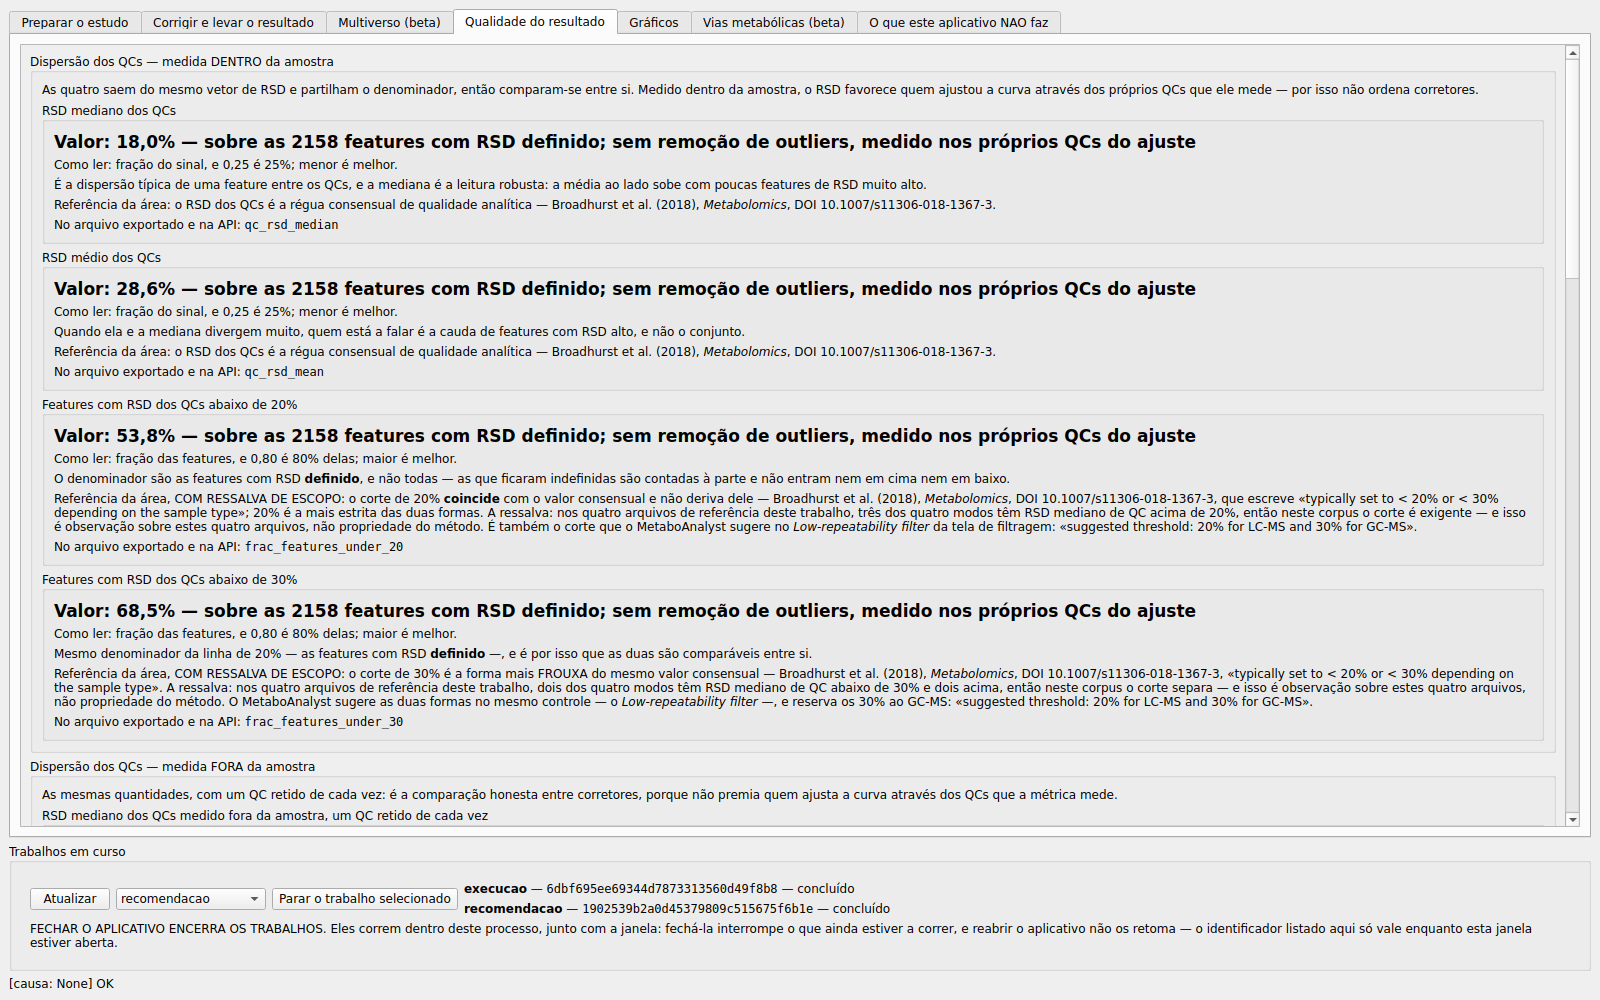
\includegraphics[width=\linewidth]{figs/cap4-aba-qualidade.png}
\fonte{Elaborado pelos autores, com o aplicativo, em 10/11/2026.}
\end{figure}

\begin{figure}[htbp]
\centering
\caption{Aba ``Gráficos'' do aplicativo, com a trajetória dos QCs ao longo da corrida}\label{fig:4-aba-graficos}
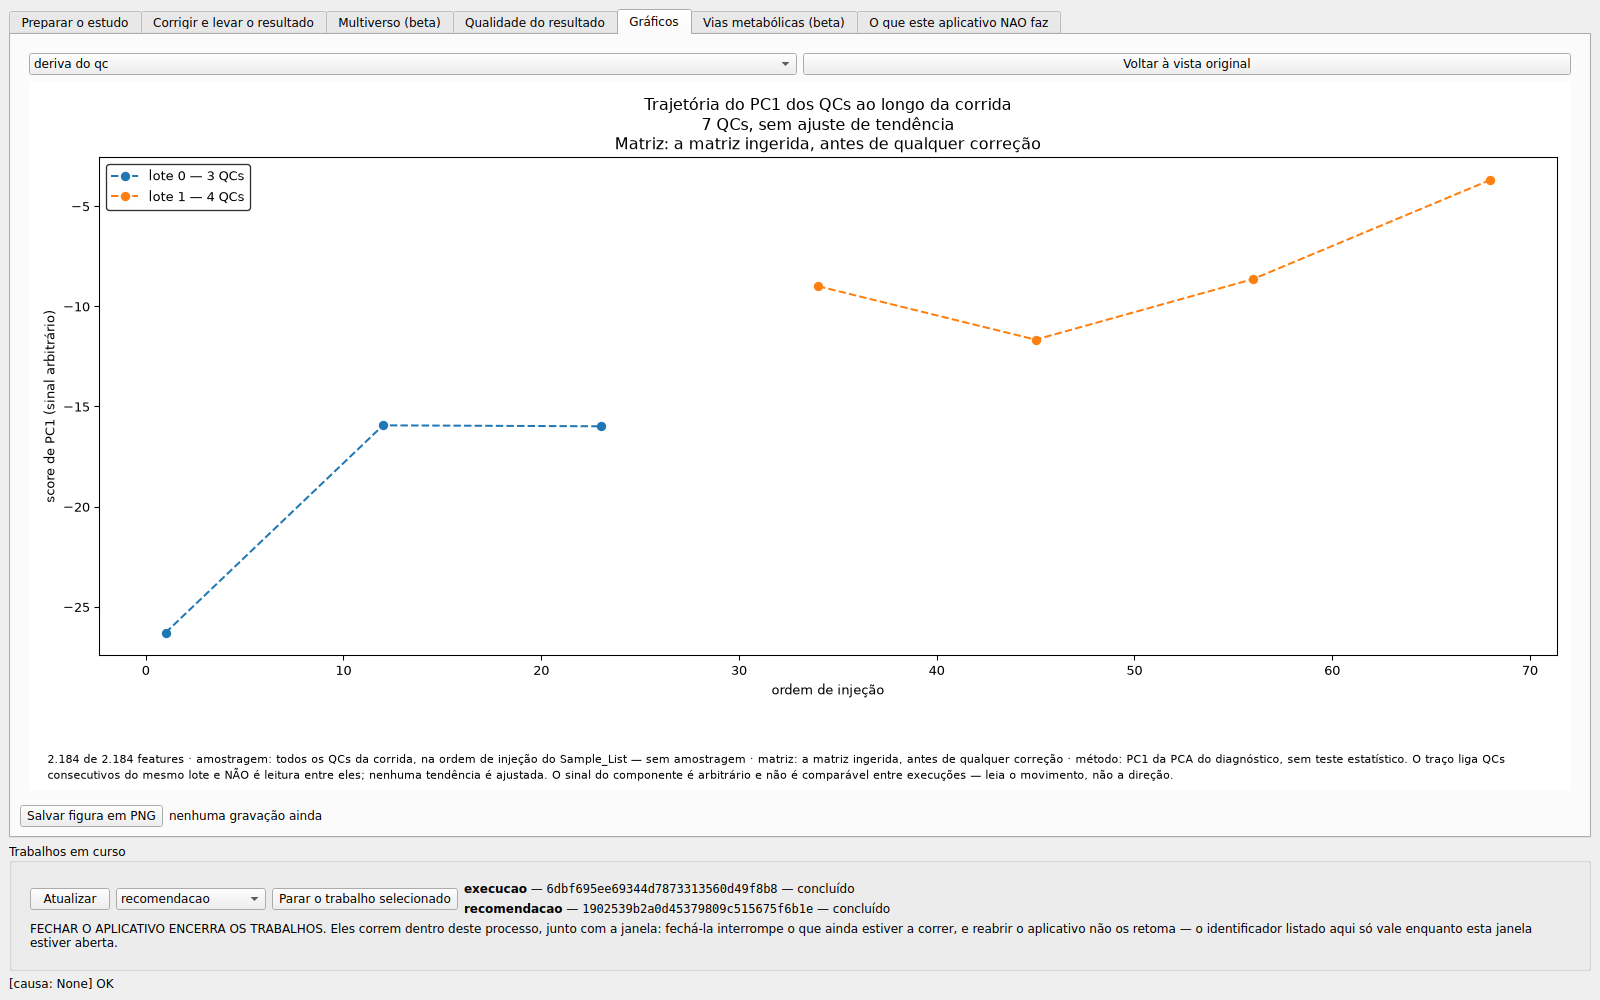
\includegraphics[width=\linewidth]{figs/cap4-aba-graficos.png}
\fonte{Elaborado pelos autores, com o aplicativo, em 10/11/2026.}
\end{figure}

A aba \textit{Preparar o estudo} concentra a seleção dos arquivos de entrada e a verificação das informações necessárias ao processamento. Nesse ponto, o usuário informa a matriz de medições e a lista de amostras correspondentes. A aplicação utiliza essas entradas para associar os valores medidos aos metadados, incluindo a ordem de injeção.

Após a seleção, o usuário pode solicitar a validação dos arquivos. Os problemas identificados são apresentados antes da execução do tratamento, permitindo revisar as inconsistências e corrigir as entradas. Essa posição da validação no fluxo evita que falhas estruturais sejam percebidas apenas durante operações de maior duração.

O diagnóstico acrescenta informações sobre o comportamento da matriz e dos controles de qualidade. Seus resultados auxiliam a escolha do método de correção e a avaliação de possíveis fronteiras de lote. As sugestões produzidas pelo sistema permanecem sujeitas à revisão do profissional.

A aba \textit{Corrigir e levar o resultado} reúne os controles de configuração e execução do processamento. O usuário pode selecionar o corretor e definir as operações posteriores, como filtragem, tratamento de valores ausentes, normalização, transformação e escalonamento. Por padrão, a caixa ``Automático'' vem marcada e aplica o corretor do palpite, medido em 200 \textit{features}; o usuário pode desmarcá-la, comparar os métodos pela medição completa e escolher o corretor.

A configuração aplicada integra o registro da execução. A organização dos controles permite relacionar o resultado aos parâmetros escolhidos, evitando que o processamento seja apresentado como uma operação única cujas decisões internas não possam ser identificadas.

A aba \textit{Qualidade do resultado} apresenta os indicadores utilizados na avaliação do tratamento. As informações são agrupadas por tema, permitindo examinar diferentes aspectos da matriz sem reduzir a qualidade a uma única medida. A apresentação considera o ponto do processamento e as condições em que cada indicador foi calculado.

A aba \textit{Gráficos} disponibiliza as representações visuais dos dados e das análises. O usuário seleciona a figura de interesse e examina aspectos como distribuição dos valores, dispersão dos controles de qualidade, estrutura multivariada e diferenças entre grupos. As figuras também podem ser exportadas para utilização em relatórios e apresentações.

A aba \textit{O que este aplicativo NÃO faz} explicita os limites das funcionalidades. Essa informação integra o fluxo de utilização porque o tratamento computacional de uma matriz não equivale à identificação de compostos, à confirmação de significado biológico ou à validação clínica dos resultados.

A área \textit{Trabalhos em curso} permanece disponível durante a navegação. Ela permite consultar o estado das operações e solicitar o cancelamento dos trabalhos que não precisam continuar. Dessa forma, o acompanhamento não fica restrito à aba em que a execução foi iniciada.

O fluxo principal de utilização pode ser organizado nas seguintes etapas:

\begin{enumerate}
    \item selecionar a matriz de medições e a lista de amostras;
    \item validar os arquivos e revisar os problemas identificados;
    \item examinar o diagnóstico e as sugestões de processamento;
    \item definir o corretor e os parâmetros de pré-processamento;
    \item iniciar a execução e acompanhar seu andamento;
    \item avaliar as métricas e os gráficos disponíveis;
    \item exportar o resultado correspondente ao ponto de processamento desejado.
\end{enumerate}

Essa sequência estabelece uma relação entre preparação, execução e avaliação. A exportação ocorre após a definição do procedimento e a obtenção de seus resultados, permitindo que o profissional examine o tratamento antes de encaminhar os dados às análises seguintes.

\subsection{Apresentação dos resultados e mensagens ao usuário}
\label{subsec:resultados-mensagens}

A apresentação dos resultados busca tornar identificáveis o procedimento aplicado, as medidas calculadas e as condições que limitam sua interpretação. A interface combina informações textuais, indicadores, tabelas e gráficos, utilizando cada representação conforme o tipo de conteúdo.

Os problemas de validação são apresentados com identificação e descrição. A distinção entre erro, aviso e informação permite reconhecer a gravidade da ocorrência e compreender se ela impede o processamento ou exige avaliação adicional. Quando disponível, a localização do problema facilita sua revisão no arquivo de origem.

As mensagens evitam tratar toda ocorrência como uma falha equivalente. Uma entrada incompatível, uma condição que exige atenção e uma operação cancelada possuem significados diferentes e precisam ser representadas de forma correspondente.

As sugestões do sistema são acompanhadas de justificativas, permitindo que o usuário examine a base da escolha antes de aceitá-la ou modificá-la. A possibilidade de sobrescrita mantém o controle metodológico com o profissional e permite registrar sua participação no processo.

A interface distingue o palpite, medido numa amostra de 200 \textit{features}, da medição completa, que aplica os corretores a todas as \textit{features}. Essa separação permite distinguir a sugestão dos resultados medidos sobre a matriz inteira.

As métricas são apresentadas com informações que contextualizam seu significado. A identificação do estimador, da população considerada e do ponto de processamento permite reconhecer o que foi medido. Essa contextualização é necessária porque indicadores com o mesmo nome podem assumir interpretações diferentes conforme o procedimento utilizado.

A organização por temas facilita a leitura do conjunto de medidas. Indicadores de repetibilidade, dispersão e estrutura dos dados são examinados de forma complementar. Uma melhoria isolada não é apresentada como comprovação de que todos os aspectos do tratamento foram aprimorados.

Os resultados das análises multivariadas são acompanhados das informações necessárias à interpretação. No caso de métodos supervisionados, as medidas de validação participam da apresentação, evitando que a separação visual entre grupos seja utilizada isoladamente como evidência de capacidade preditiva.

Os gráficos preservam a identificação dos grupos e dos controles de qualidade quando essas informações participam da análise. Títulos, eixos e legendas indicam as quantidades representadas, permitindo relacionar a figura aos dados utilizados em sua construção.

Quando uma figura não pode ser produzida com as informações disponíveis, a interface apresenta essa condição. A ausência de dados necessários não deve resultar na exibição de uma imagem que sugira uma análise válida ou na manutenção de uma figura pertencente a uma execução anterior.

A apresentação também acompanha o estado dos trabalhos. Uma operação em andamento é diferenciada de uma operação concluída, cancelada ou encerrada com falha. O resultado é disponibilizado de acordo com o desfecho correspondente, mantendo a associação entre a solicitação e o artefato recuperado.

As mensagens sobre cancelamento consideram que a solicitação pode depender de um ponto de verificação do processamento para ser atendida. Por isso, solicitar a interrupção e concluir o cancelamento são condições distintas.

As limitações metodológicas permanecem visíveis ao usuário. O aplicativo trata matrizes de sinais analíticos e fornece recursos de avaliação computacional, mas a interpretação científica exige considerar o desenho do estudo e as evidências disponíveis. A apresentação dos resultados deve preservar essa distinção.

\subsection{Empacotamento e distribuição para Windows}
\label{subsec:empacotamento-windows}

O empacotamento foi realizado com PyInstaller, que reúne o código da aplicação, o interpretador Python, as bibliotecas e os recursos necessários à execução. O pacote resultante utiliza o formato de diretório, contendo o arquivo \texttt{refino.exe} e os componentes que sustentam seu funcionamento.

A distribuição em pasta permite iniciar a aplicação após a extração do arquivo compactado. O usuário não precisa instalar Python, executar comandos de preparação do ambiente ou configurar um servidor de banco de dados para utilizar o fluxo principal.

O executável inicia a interface gráfica e a API interna utilizada para acionar as funcionalidades. A comunicação ocorre em endereço local, e o aplicativo administra a inicialização dos componentes necessários. O banco SQLite atende à persistência sem depender de um serviço externo.

O conteúdo distribuído inclui as bibliotecas numéricas, os componentes da interface e os recursos utilizados na apresentação dos resultados. A seleção dos componentes considera as dependências efetivamente necessárias ao aplicativo, evitando incorporar ao pacote todo o ambiente de desenvolvimento.

O processo de empacotamento exige verificar o comportamento do produto gerado. A execução pelo código-fonte e a execução pelo aplicativo congelado possuem diferenças relacionadas à localização dos recursos, ao carregamento de bibliotecas e à disponibilidade de arquivos auxiliares. Por esse motivo, a verificação considera o funcionamento dentro da própria pasta de distribuição.

Entre os aspectos avaliados estão a abertura da janela, a disponibilidade das funcionalidades, a geração dos artefatos e a apresentação dos gráficos. Essas verificações permitem identificar problemas que não seriam observados apenas pela execução dos testes no ambiente de desenvolvimento.

A apresentação de textos também é considerada no produto empacotado. Mensagens e conteúdos com caracteres acentuados precisam permanecer legíveis no executável, preservando a compreensão das instruções e dos resultados pelo usuário.

O pacote público exclui os arquivos produzidos durante a utilização, incluindo o banco de dados, os registros de execução em arquivo e a pasta de saídas. Esses elementos podem conter informações associadas às amostras e não são necessários para distribuir o programa.

A separação entre aplicação e dados evita que uma cópia utilizada no desenvolvimento seja publicada com resultados ou metadados do laboratório. O material distribuído contém os componentes de software necessários à execução, enquanto os arquivos do estudo são fornecidos e utilizados no contexto apropriado.

A distribuição é acompanhada de instruções de utilização em um arquivo de leitura inicial. Esse material orienta a extração do pacote e a abertura do executável, permitindo que o usuário identifique o ponto de entrada da aplicação.

As versões distribuídas recebem identificação própria e podem ser relacionadas ao estado do código-fonte utilizado em sua geração. A conferência por soma de verificação permite comparar a integridade do arquivo compactado com o artefato produzido no empacotamento.

O aplicativo não utiliza instalador nem assinatura de código. Essas características fazem parte do formato de distribuição adotado e são informadas ao usuário. A utilização ocorre diretamente a partir da pasta extraída, que precisa conter os recursos necessários e permitir as operações locais de escrita realizadas pelo sistema.

\subsection{Repositório do código-fonte}
\label{subsec:repositorio-codigo-fonte}

O código-fonte do MetaRefino é mantido em um repositório com controle de versão Git. O versionamento permite acompanhar as alterações realizadas durante o desenvolvimento e identificar o estado do projeto utilizado na geração de uma versão da aplicação.

O repositório reúne o código da interface, os componentes de processamento, os módulos de persistência, as migrações, os testes e os scripts de empacotamento. Também contém os materiais necessários à compreensão da organização do projeto e à preparação do ambiente de desenvolvimento.

A estrutura separa os componentes por responsabilidade, distinguindo o domínio, as operações científicas, a entrada e saída de arquivos, a persistência e a apresentação. Essa organização facilita a localização das funcionalidades e permite relacionar alterações aos componentes afetados.

Os registros de versão contribuem para a manutenção e a rastreabilidade técnica. Uma versão distribuída pode ser associada a um estado específico do código, permitindo identificar quais alterações estão presentes no executável correspondente.

O código adota a licença GPL-3.0-or-later. A licença do software não abrange automaticamente os dados científicos utilizados no desenvolvimento. Os arquivos pertencentes ao laboratório exigem tratamento separado e não devem ser considerados disponíveis para redistribuição apenas por terem sido utilizados na avaliação da aplicação.

O endereço do repositório do projeto é apresentado a seguir:

\begin{quote}
    \textbf{Repositório do código-fonte:} \url{github.com/NishiyaKN/refino-quimiometrico}
\end{quote}

% Seção «Inteligência Artificial e Decisões Automatizadas», versão LaTeX (abnTeX2).
% Gerada do corpo de docs/secao-ia-decisoes-automatizadas.md (sha256 0ca45d4c8e28916e) por
% scripts/gera_secao_ia_latex.py, com pandoc 3.1.3.
% NÃO EDITE AQUI: edite o .md e gere de novo. O .md é a fonte, e a conferência
% de cada número está nele. Para o Overleaf: colar este arquivo inteiro no
% capítulo escolhido (ele começa em um \section); as
% 20 referências novas estão em secao-ia-decisoes-automatizadas.bib, e as
% outras 4 citadas já estão no .bib do Overleaf. Requer a classe abntex2
% (\fonte e \nota) e o abntex2cite (\cite); nenhum pacote a mais.

% A classe abntex2 traz \fonte e \nota, mas não o ambiente quadro: quem o define
% é o preâmbulo do modelo do abnTeX2. Se o do Overleaf já o tiver, as linhas abaixo
% não fazem nada.
\makeatletter
\@ifundefined{quadro}{%
  \providecommand{\quadroname}{Quadro}%
  \newfloat{quadro}{loq}{\quadroname}%
}{}
\makeatother
% As tabelas e o quadro desta seção não flutuam: ficam no lugar do texto, sem cortar
% parágrafo. A legenda fixa é a da memoir, a base do abntex2, e numera e entra na lista
% como a legenda de sempre.
\providefixedcaption{\tabelafixa}{table}
\providefixedcaption{\quadrofixo}{quadro}
\section{Inteligência Artificial e Decisões Automatizadas}

Na ferramenta desenvolvida, algoritmos de inteligência artificial apoiam as decisões metodológicas do refino quimiométrico, e esse apoio se concentra nas escolhas que antecedem o processamento de uma corrida analítica: a forma do erro sistemático presente nos dados, o número de lotes analíticos a declarar e o método de correção de sinal a aplicar. Declarar lotes significa dividir a corrida em trechos, cada um corrigido com seus próprios QCs.

Escolher, a partir de características mensuráveis de uma instância, o algoritmo com o melhor desempenho esperado sobre ela é o chamado problema de seleção de algoritmos \cite{rice1976algorithm}. Aprender essa escolha com base em experiências anteriores é o objeto do meta-aprendizado, uma das bases do aprendizado de máquina automatizado (AutoML) \cite{brazdil2022metalearning}. Em metabolômica, ferramentas como o NormalizeMets comparam métodos de normalização sobre os dados do próprio usuário \cite{de2018normalizemets}, e o aprendizado de máquina tem sido aplicado à modelagem de doenças e à classificação de amostras \cite{galal2022applications}.

Na ferramenta, o apoio à decisão combina mecanismos de naturezas diferentes. O diagnóstico do erro sistemático é um classificador baseado em regras, construído e calibrado neste trabalho. A escolha do corretor, nome dado aqui ao método de correção de sinal, foi estudada primeiro como um modelo de aprendizado de máquina e acabou resolvida por medição, como se descreve adiante. O aprendizado de máquina aparece ainda dentro dos próprios métodos de correção e de análise.

O princípio que orientou o desenho desses pontos é que a decisão automática funcione como uma segunda opinião. As propostas chegam ao usuário com a justificativa e podem ser aceitas ou alteradas, e cada execução fica registrada com a escolha efetivamente usada. Esse cuidado se justifica porque auxílios à decisão imperfeitos levam a dois tipos de erro: no de omissão, o usuário deixa de notar um problema que o auxílio não apontou, e no de comissão, segue uma recomendação errada sem verificá-la. Os dois caracterizam o viés de automação, que não é evitado por treinamento nem por instruções \cite{parasuraman2010complacency}. O Quadro~\ref{quadro:ia-decisoes} resume os pontos em que o aplicativo decide ou propõe algo no lugar do usuário.

\par\medskip
\noindent\begin{minipage}{\linewidth}
  \quadrofixo{Pontos de decisão automática do aplicativo}
  \label{quadro:ia-decisoes}
  \centering
  \footnotesize
  \setlength{\tabcolsep}{3pt}
  \begin{tabular}{|>{\raggedright\arraybackslash}p{1.9cm}|>{\raggedright\arraybackslash}p{3.0cm}|>{\raggedright\arraybackslash}p{3.1cm}|>{\raggedright\arraybackslash}p{3.0cm}|>{\raggedright\arraybackslash}p{2.7cm}|}
    \hline
    \textbf{Ponto de decisão} & \textbf{O que a máquina propõe ou decide} & \textbf{Mecanismo} & \textbf{O que o usuário vê} & \textbf{Controle do usuário} \\
    \hline
    Diagnóstico & a classe do erro sistemático e as fronteiras de lote; o número de lotes é pré-preenchido & sequência ordenada de regras sobre o RSD dos QCs e sobre os componentes principais, com detecção de pontos de mudança na trajetória dos QCs & classe, confiança, pontos de corte e número de QCs em cada lote proposto & altera o número de lotes; mantido o proposto, a correção corta nas fronteiras propostas \\
    \hline
    Palpite (a sugestão de corretor) & o corretor (não corrigir, LOESS ou SERRF) e a confiança na escolha, ou o empate & a mesma validação da linha seguinte, em 200 \emph{features} sorteadas da matriz & corretor, confiança e justificativa & caixa ``Automático'', marcada por padrão, ou escolha manual \\
    \hline
    Medir qual corretor vence & a opção de menor RSD dos QCs fora da amostra, inclusive não corrigir, ou a abstenção & validação que retira um QC por vez, nas três opções, com os lotes declarados & RSD de cada opção, margem, abstenção e se o palpite coincidiu & nenhum: o resultado é exibido e não altera os controles \\
    \hline
    Teste univariado & teste \emph{t} de Welch ou teste de Mann-Whitney & teste de normalidade de Shapiro-Wilk sobre os desvios dentro dos grupos & o teste escolhido e o \emph{p}-valor do teste de normalidade, no gráfico de vulcão & a janela não permite escolher o teste \\
    \hline
  \end{tabular}
  \fonte{elaborado pelos autores.}
\end{minipage}
\par\medskip

\subsection{Diagnóstico automático do erro sistemático}

O estudo usado neste trabalho tem quatro corridas, uma por modo analítico. Cada modo combina uma coluna cromatográfica (HILIC, de interação hidrofílica, ou C18, de fase reversa) com uma polaridade de ionização, positiva ou negativa. A análise exploratória mostrou que o erro sistemático não tem a mesma forma nas quatro. Projetados no primeiro componente principal, os QCs do HILIC negativo mudam de nível entre as injeções 45 e 56 e permanecem deslocados, os do C18 negativo se deslocam de forma gradual e os dos dois modos positivos oscilam sem padrão monotônico. Os métodos de correção partem de premissas diferentes sobre essa forma. A regressão local (LOESS) ao longo da ordem de injeção supõe uma deriva suave, e um degrau só é corrigido se as duas partes da corrida forem declaradas como lotes distintos. Por isso, a ferramenta classifica o tipo de defeito antes de propor a correção.

A diretriz de consenso de Broadhurst e colaboradores recomenda inspecionar o RSD de cada metabólito nos QCs, a posição dos QCs no gráfico de escores dos dois primeiros componentes principais e a resposta dos metabólitos ao longo da ordem de injeção \cite{broadhurst2018guidelines}. As recomendações do QComics acrescentam cartas de controle com as regras de Westgard, que detectam medições fora de controle \cite{doi:10.1021/acs.analchem.3c03660}. Essas regras indicam se a corrida saiu de controle, mas não qual é a forma do erro, e, com sete QCs por corrida, a que exige dez pontos consecutivos do mesmo lado da média nem chega a ser aplicável. A distinção entre formas de erro tem precedente em proteômica, em que se separam efeitos de lote contínuos, corrigidos por regressão ao longo da ordem das corridas, de efeitos discretos, corrigidos por centragem \cite{cuklina2021diagnostics}. Neste trabalho, essa separação é aplicada à matriz inteira por uma sequência de regras com limiares explícitos.

O diagnóstico transforma as inspeções da diretriz em quatro grandezas, calculadas sobre a matriz ainda não corrigida. A primeira é a mediana, entre as \emph{features}, do RSD dos QCs, calculado sobre as intensidades sem transformação e com a mesma remoção de valores discrepantes que o pipeline do laboratório aplica. As outras três vêm da análise de componentes principais da matriz transformada por \(\log_{10}(1 + x)\) e autoescalonada: a correlação de Spearman, em valor absoluto, entre o primeiro componente e a ordem de injeção; a razão entre a dispersão dos QCs e a das amostras nos dois primeiros componentes; e a trajetória dos QCs no primeiro componente. A agregação pela mediana e a correlação com a ordem de injeção são resumos construídos neste trabalho, já que a diretriz de Broadhurst e colaboradores descreve as inspeções metabólito a metabólito ou por gráfico. A correlação com a ordem de injeção e a razão de dispersão são ainda recalculadas sob pequenas perturbações dos escores, com semente fixa, e uma métrica indefinida ou instável não é usada para classificar.

As regras são avaliadas em ordem fixa, e a primeira que se aplica decide a classe:

\begin{enumerate}
\item
  \emph{não avaliável}, quando as métricas de componentes principais são indefinidas ou instáveis, ou quando a trajetória dos QCs quase não se move, o que corresponde a uma abstenção do diagnóstico;
\item
  \emph{limpo}, quando a mediana do RSD dos QCs fica abaixo do limiar do modo e a correlação do primeiro componente com a ordem de injeção fica abaixo de 0,30;
\item
  \emph{mudança em degrau}, quando há ponto de mudança na trajetória dos QCs e o novo nível se sustenta, isto é, quando a diferença entre as médias dos dois segmentos é mais que o dobro da maior amplitude interna a eles;
\item
  \emph{deriva gradual}, quando a trajetória é predominantemente monotônica, com razão de 0,487 ou mais entre o deslocamento líquido e o deslocamento total;
\item
  \emph{errático}, nos demais casos.
\end{enumerate}

Cada classificação traz uma confiança, calculada pela distância relativa entre o valor medido e o limiar que decidiu. Uma decisão tomada perto do limiar recebe confiança baixa, e esse valor não é uma probabilidade. O limiar de RSD da regra de limpeza é calibrado por modo, sobre matrizes sintéticas, com a restrição de manter nas corridas reais as classes vistas na análise exploratória: ele fica em cerca de 105\% no HILIC positivo, 23\% no C18 positivo, 49\% no HILIC negativo e 16\% no C18 negativo. Como acompanha o nível de RSD de cada modo, a classe limpo indica que a corrida não se afasta do nível do seu modo nem acompanha a ordem de injeção, e não que sua variabilidade seja baixa. Para um modo que a ferramenta não conhece, vale o corte de 20\%, o mais estrito dos dois, 20\% e 30\%, que a diretriz cita \cite{broadhurst2018guidelines}. Os limiares foram escolhidos a partir de medições sobre as quatro corridas e são próprios desses dados, e não constantes gerais do método. Com sete QCs, a regra da deriva gradual tem ainda um limite estatístico: em simulação, 36\% das trajetórias de um passeio aleatório puro, lidas nas posições dos sete QCs, já passam de 0,487, e subir o limiar não separaria a deriva do passeio aleatório.

Para propor fronteiras de lote, o diagnóstico procura pontos de mudança na trajetória dos QCs por segmentação binária, com um modelo constante em cada segmento \cite{truong2020selective}. Um corte é aceito quando reduz a soma dos quadrados dos resíduos em mais que uma penalidade de vinte vezes a variância do ruído. O ruído é estimado pelas diferenças entre QCs consecutivos, que um degrau quase não altera. O fator 20 fica perto do centro, em escala logarítmica, da faixa de 2,5 a 200 em que o detector acertou os casos de teste construídos e manteve um único corte no HILIC negativo. Como a trajetória tem um ponto por QC, cada corte é uma hipótese sobre poucos pontos, e a janela o apresenta como sugestão, com o número de QCs de cada lote proposto. Nas corridas reais, o detector propõe dois lotes no HILIC negativo, com o corte antes da injeção 56, dois no C18 negativo, um no C18 positivo e três no HILIC positivo. A busca de fronteiras corre independentemente da classe do defeito. Quando o usuário mantém o número proposto, a correção divide a corrida nessas fronteiras; se ele o altera, a corrida é dividida em blocos contíguos de tamanho quase igual. A diferença pode ser grande: no HILIC negativo, dois blocos iguais separam as injeções 34 e 35, e o degrau ficaria dentro do segundo lote.

Também foi testado se declarar dois lotes no HILIC negativo, com a fronteira logo depois da injeção 45, o último QC antes do degrau, reduz a correlação do primeiro componente com a ordem de injeção depois do SERRF. A correlação caiu de 0,61, com um lote, para 0,18, com dois. Em vários outros pontos de corte, porém, a redução foi igual ou maior: dos outros 43 cortes que deixam ao menos dois QCs em cada lote, 17 deram correlação menor, a maioria com o segundo lote começando perto do meio da corrida. A redução, portanto, não mostra que o degrau foi corrigido. A menor correlação de todas, 0,08, veio dos cortes antes das injeções 55 e 56, o segundo deles o proposto pelo detector. Nesses cortes, o segundo componente passa a ter correlação de 0,84 a 0,92 com a ordem de injeção, e a ordem continua pesando nos dados.

Nas corridas reais, o diagnóstico classifica o HILIC negativo como mudança em degrau, o C18 negativo como limpo e os dois modos positivos como erráticos. O C18 negativo sai como limpo, apesar da deriva vista na análise exploratória, porque o RSD mediano dos seus QCs fica abaixo do limiar do modo e o primeiro componente quase não acompanha a ordem de injeção. Essas classificações não medem o desempenho do método, porque os limiares foram escolhidos para reproduzi-las e a forma verdadeira do erro nessas corridas não é conhecida. O desempenho foi medido em matrizes produzidas pelo gerador de dados sintéticos desenvolvido neste trabalho, que reamostra os resíduos das corridas reais e injeta um defeito de forma e intensidade conhecidas, o que permite avaliar o método contra uma resposta conhecida de antemão \cite{morris2019using}. A intensidade é dada pela razão entre a amplitude da deriva e a variação de fundo de cada \emph{feature}.

Em 200 matrizes com sete QCs, 50 de cada classe, e razão de 0,8, a classe correta foi recuperada em 139 (69,5\%), contra 25\% esperados ao acaso. O acerto é alto nas matrizes limpas (46 de 50) e mais baixo na mudança em degrau (26 de 50). Ele depende da intensidade do defeito: com razões de 0,2, 0,4, 1,5 e 3,0, foi de 35,0\%, 46,0\%, 88,0\% e 88,5\%. Com deriva fraca, a maior parte das matrizes com defeito é classificada como limpa ou errática; com deriva forte, o degrau e a deriva gradual são reconhecidos em todas as matrizes, e os erros se concentram nas erráticas. O acerto também varia com o modo de origem, de 50,0\% nas matrizes derivadas do HILIC positivo a 91,7\% nas do C18 negativo, e cai para 58,0\% quando se usa o limiar de reserva de 20\%, o de um modo desconhecido. A confiança declarada acompanha o acerto: nas 800 matrizes distintas das cinco razões (as 50 limpas são comuns a todas), a classe está certa em 29,5\% das vezes com confiança abaixo de 0,1 e em 69,6\% com confiança a partir de 0,3.

A proposta de lotes foi avaliada nas mesmas matrizes. Numa matriz em degrau, o corte certo é o que inicia um lote no primeiro QC posterior ao degrau. Nas 50 matrizes em degrau de cada razão, da 0,2 à 3,0, o detector propôs só o corte certo em 4, 7, 31, 46 e 47 delas. Como independe da classe, a proposta também divide matrizes sem degrau: recebem algum corte 9 das 50 limpas e, na razão 0,8, 35 das 50 de deriva gradual. Daí a janela mostrar o número de QCs de cada lote e deixar o número de lotes sob controle do usuário.

O diagnóstico não escolhe o corretor. Nas 88 matrizes sintéticas usadas na escolha do corretor, descrita a seguir, todas com deriva gradual injetada, o SERRF venceu pela medida dos QCs em todas as classes que o diagnóstico atribuiu: em 15 das 17 classificadas como limpas, 22 das 24 erráticas, 35 das 46 de deriva gradual e na única em degrau. O tipo de defeito, sozinho, não indica o corretor, e a ferramenta não usa uma regra que associe um ao outro.

\subsection{Escolha automática do corretor}

A segunda decisão automática é a escolha entre as três opções de correção de sinal. A primeira é não corrigir, que é uma opção legítima, porque a correção também pode piorar o dado. A segunda é o LOESS, ajustado aos QCs ao longo da ordem de injeção, na linha da correção proposta por Dunn e colaboradores \cite{dunn2011procedures}. A terceira é o SERRF \cite{fan2019systematic}, que modela o erro de cada \emph{feature} com uma floresta aleatória treinada nos QCs. Das etapas do pré-processamento, só o corretor é escolhido automaticamente; as demais seguem os padrões declarados da ferramenta ou a escolha do usuário.

No fluxo anterior do laboratório, a correção roda no pipeline em R, que aplica o SERRF e o LOESS, e a escolha entre eles é feita olhando o resultado. Segundo a equipe, espera-se que, depois de uma boa correção, os QCs apareçam agrupados e no centro do gráfico de componentes principais, e escolhe-se o corretor com que os QCs ficaram mais agrupados e com menor RSD. O pipeline grava, junto das matrizes corrigidas, um gráfico de barras do RSD dos QCs e o gráfico de componentes principais. O RSD das barras é medido em dois QCs retirados do ajuste, em cinco sorteios sem semente, e por isso muda de uma execução para outra. O agrupamento no gráfico, ao contrário, avalia a correção nos próprios QCs que a ajustaram, e o LOESS, que ajusta uma curva aos QCs, reduz a variação justamente neles. O artigo do SERRF já advertia que o desempenho devia ser avaliado em amostras que não participaram do treinamento \cite{fan2019systematic}.

A ferramenta adota uma medida fora da amostra que se repete. Cada QC é retirado por vez, o corretor é reajustado com os demais e o RSD é calculado sobre os valores corrigidos dos QCs retirados. O corretor de menor mediana desse RSD, entre as \emph{features}, é o vencedor, e quando a segunda melhor opção fica a menos de 1,2\% da melhor, em termos relativos, a medição se abstém. Esse limiar vem do ruído da própria medida. Repetida com 21 sementes diferentes nos quatro arquivos reais, a margem entre as duas melhores opções teve desvio-padrão de 0,20\% a 0,51\%, conforme o arquivo, e em nenhum deles a troca de semente mudou o vencedor. O dobro do maior desses desvios dá 1,03\%, com intervalo de 95\% por reamostragem de 0,82\% a 1,24\%, e o limiar de 1,2\% fica dentro dele: uma margem abaixo disso não se distingue do que a troca de semente produz sozinha. No C18 negativo, onde a margem é a menor dos quatro, uma das 21 sementes a deixou abaixo do limiar, e a medição teria se abstido.

A primeira versão da escolha automática tentava prever esse vencedor sem corrigir a matriz, como no problema de seleção de algoritmos. Era uma política aprendida, treinada em matrizes sintéticas, porque o estudo tem só quatro corridas reais. O conjunto usado para avaliá-la reúne 88 matrizes, 22 derivadas de cada modo, com 2.000 \emph{features}, sete QCs nas posições das corridas reais e razão entre deriva e ruído sorteada, em escala logarítmica, entre 0,1 e 3,0. Cada matriz recebe como rótulo o vencedor da medida fora da amostra, o que exige reajustar os três corretores uma vez para cada QC retirado.

As entradas da política são 17 características que o diagnóstico calcula da matriz bruta, como a mediana e o percentil 75 do RSD dos QCs, a fração de zeros, a correlação do primeiro componente com a ordem de injeção, a razão de dispersão dos QCs, a confiança e o tipo de defeito. Ficam de fora, de propósito, as grandezas que dependem de executar os corretores. Se a política pudesse lê-las, a resposta já seria conhecida antes da recomendação, e a avaliação seria contaminada por informação indisponível no momento da decisão, o que se conhece como vazamento \cite{kaufman2012leakage}. O modelo é formado por duas árvores de decisão do tipo CART \cite{breiman1984classification}: uma classifica o corretor, e a outra prediz a margem entre o melhor e o segundo, de onde sai a confiança. A profundidade foi limitada a três níveis para que o caminho da raiz até a folha, com a característica, o valor medido e o limiar de cada nó, sirva de justificativa da decisão, como recomenda o uso de modelos interpretáveis quando a decisão tem consequências \cite{rudin2019stop}.

A política foi comparada com a regra mais simples possível, escolher sempre o SERRF, o corretor que vence em 73 das 88 matrizes. Como as duas julgam as mesmas matrizes, a diferença foi avaliada pelo teste exato de McNemar sobre os casos em que discordam \cite{mcnemar1947note}, indicado para comparar dois classificadores no mesmo conjunto de teste \cite{dietterich1998approximate}. O desempenho foi estimado de três formas. Avaliada nas próprias matrizes do treinamento, a política acerta 78. Retirando uma matriz por vez, acerta 65, menos que a regra fixa, com 10 discordâncias contra e 2 a favor (\emph{p} = 0,04). Retirando todas as matrizes de um modo e julgando esse modo com o modelo treinado nos outros três, acerta 72, contra 73, com uma única discordância. Esta última forma é a que importa, porque matrizes do mesmo modo compartilham a estrutura de correlação, o padrão de zeros e o perfil dos QCs, e separar treinamento e teste por matriz deixa essa informação dos dois lados \cite{roberts2017cross}. A política e a regra fixa quase não discordam nessa forma de avaliação, e nenhuma versão, nesta nem nas treinadas antes, mostrou vantagem estatisticamente detectável sobre ela. A política aprendida continua disponível pela linha de comando, mas deixou de ser a sugestão do aplicativo.

O palpite, nome que o aplicativo dá à sugestão de corretor, passou então a medir. O aplicativo aplica as três opções a 200 \emph{features} sorteadas da matriz do usuário, com semente fixa, e propõe a de menor RSD dos QCs fora da amostra. Ele continua sendo um palpite, porque mede uma amostra e não todas as \emph{features}, mas agora apoiado numa medição. A escolha de 200 \emph{features} considerou o custo, que cresce linearmente com o número de \emph{features}, e uma simulação sobre os valores por \emph{feature} já medidos nas 88 matrizes sintéticas, que têm todas deriva gradual. Refeita com o código atual, com 200 sorteios por matriz, a concordância com a medição de todas as \emph{features} foi de 86,1\% com 50 \emph{features}, 89,6\% com 100, 93,1\% com 200 e 95,6\% com 500, enquanto escolher sempre o SERRF acertaria 73 das 88 matrizes (83,0\%). Com 200, quando a amostra erra, o RSD da opção escolhida fica em média cerca de 4\% acima do da melhor, em diferença relativa; somados todos os sorteios, a diferença média é de 0,28\%.

Quando a diferença relativa entre as duas melhores opções na amostra fica abaixo de cerca de 17\%, o dobro do maior desvio-padrão dessa diferença entre sorteios nos quatro arquivos reais, o palpite declara empate, mas mantém a proposta. Esse limiar é bem mais largo que o de 1,2\% da medição de todas as \emph{features}, porque, com 200 \emph{features}, a diferença muda muito mais de um sorteio para outro do que com a troca de semente. Substituir a proposta pelo SERRF nos empates foi avaliado, num outro conjunto de sorteios, e aumentou a diferença média para a melhor opção de 0,26\% para 0,78\%. Nos quatro arquivos reais, o palpite propôs o mesmo corretor que a medição de todas as \emph{features}, e em dois deles, o HILIC negativo e o C18 negativo, declarou empate. Num computador de 12 núcleos lógicos, ele levou menos de um minuto por arquivo.

A caixa ``Automático'' do corretor vem marcada e entrega a escolha ao palpite no momento da execução. Quem executa sem alterar nada recebe o corretor do palpite, e nesse uso a decisão automática deixa de ser segunda opinião e passa a ser a escolha. Por isso, ao fim da execução, a janela informa qual corretor foi aplicado e quem o escolheu. Para quem quer o resultado completo, o botão ``Medir qual corretor vence'' aplica a mesma medida a todas as \emph{features}, com os lotes declarados. No mesmo computador, com um lote, essa medida levou de 8,6 minutos (HILIC negativo) a 27 minutos (HILIC positivo). Como cada QC retirado precisa de pelo menos dois outros no mesmo lote, ela recusa uma divisão com menos de três QCs em algum lote, o que, com sete QCs, admite no máximo dois lotes. A proposta do detector não pôde ser medida no HILIC negativo (5 e 2 QCs) nem no HILIC positivo (2, 2 e 3). Nas divisões em dois lotes que puderam ser medidas, no C18 negativo e em blocos iguais no HILIC negativo, nenhuma superou o lote único.

Cada execução fica registrada no banco de dados local do aplicativo, com a configuração efetivamente usada e a justificativa da escolha. Quando o usuário altera um valor proposto, o registro guarda também a proposta da máquina e quais parâmetros foram alterados, e a substituição de uma proposta pode ser contada depois. Manter a proposta sem mexer no controle, porém, não se distingue de avaliá-la e mantê-la, e nenhuma sessão de uso por especialista foi registrada até aqui.

Nos quatro arquivos reais, com um lote, a medição elegeu o SERRF no HILIC positivo, no C18 positivo e no C18 negativo, e o LOESS no HILIC negativo. As medianas estão na Tabela~\ref{tab:ia-reais}, ao lado das do pipeline do laboratório.

\subsection{O SERRF e o LOESS da ferramenta e os do laboratório}

O SERRF da ferramenta é uma reimplementação do original em R. A floresta aleatória \cite{breiman2001random} de cada \emph{feature} é treinada apenas nos QCs e prevê a intensidade a partir das dez \emph{features} mais correlacionadas com ela \cite{fan2019systematic}. As duas implementações diferem em reprodutibilidade. O SERRF do pipeline em R não fixa semente e substitui os zeros por valores sorteados, de modo que duas execuções sobre o mesmo arquivo não dão o mesmo resultado. O LOESS do pipeline também tem partes sorteadas sem semente, e, quando mais de um quinto da curva ajustada de uma \emph{feature} sai negativa, devolve a \emph{feature} sem correção e sem avisar, o que, numa execução, aconteceu em 1.561 das 6.035 \emph{features} do HILIC positivo (25,9\%). Na ferramenta, toda operação aleatória recebe uma semente derivada da semente geral e da \emph{feature} (no SERRF, também do lote e do passo), a mesma entrada dá sempre a mesma saída, e as \emph{features} que o LOESS deixa sem correção ficam marcadas.

A diferença tem consequência prática no fluxo anterior, em que as \emph{features} com RSD dos QCs acima de um corte, como 20\%, são descartadas antes da análise estatística. Numa medição à parte, com cinco execuções do pipeline em R sobre o mesmo arquivo do HILIC positivo, em média 84 das 6.035 \emph{features} mudaram de lado do corte de 20\% entre duas execuções do SERRF, e 657 entre duas do LOESS. Nos outros três modos, as trocas foram de 6 a 15 \emph{features} com o SERRF e de 117 a 218 com o LOESS. A mesma análise, repetida sobre o mesmo arquivo, pode assim trabalhar com conjuntos diferentes de \emph{features}. Na ferramenta, duas execuções com a mesma entrada dão a mesma matriz.

A floresta da ferramenta passou por duas versões, e uma terceira foi testada. A primeira, com os parâmetros da biblioteca scikit-learn, corrigia bem menos que o R: no C18 positivo, deixava o RSD dos QCs fora da amostra em 21,55\%, contra 15,35\% do R. A causa era uma diferença de semântica. O tamanho mínimo para dividir um nó conta, no scikit-learn, as amostras distintas do sorteio com reposição e, no pacote ranger, usado pelo SERRF em R, os sorteios. Com sete QCs, cerca de 40\% das árvores da primeira versão não faziam divisão nenhuma. A floresta atual passa à árvore as amostras repetidas, como o ranger, e chega perto do R (Tabela~\ref{tab:ia-reais}): nos quatro modos ela corrige um pouco mais que ele, e em todos a diferença fica abaixo de um ponto percentual. Permitir ainda mais divisões por árvore afastaria mais, por exemplo 12,49\% contra 15,35\% do R no C18 positivo. A versão atual foi escolhida por ficar mais próxima do pipeline a que o laboratório está acostumado.

\par\medskip
\noindent\begin{minipage}{\linewidth}
  \tabelafixa{Mediana do RSD dos QCs fora da amostra (\%) nos quatro arquivos reais, com um lote}
  \label{tab:ia-reais}
  \centering
  \footnotesize
  \setlength{\tabcolsep}{3pt}
  \begin{tabular}{>{\raggedright\arraybackslash}p{2.0cm}>{\raggedright\arraybackslash}p{1.7cm}>{\raggedright\arraybackslash}p{1.9cm}>{\raggedright\arraybackslash}p{2.3cm}>{\raggedright\arraybackslash}p{1.9cm}>{\raggedright\arraybackslash}p{1.8cm}>{\raggedright\arraybackslash}p{2.3cm}}
    \hline
    \textbf{Modo} & \textbf{Sem correção} & \textbf{LOESS, ferramenta} & \textbf{LOESS, pipeline em R} & \textbf{SERRF, primeira versão} & \textbf{SERRF, versão atual} & \textbf{SERRF, pipeline em R} \\
    \hline
    HILIC positivo & 143,81 & 147,43 & 142,34 a 142,67 & 135,69 & 109,92 & 110,34 a 110,39 \\
    C18 positivo & 24,15 & 32,40 & 30,42 a 30,62 & 21,55 & 14,38 & 15,35 a 15,37 \\
    HILIC negativo & 67,18 & 59,20 & 59,57 a 59,80 & 66,08 & 61,45 & 61,63 a 62,10 \\
    C18 negativo & 15,50 & 19,32 & 18,76 a 19,19 & 15,45 & 15,12 & 15,17 a 15,37 \\
    \hline
  \end{tabular}
  \fonte{elaborado pelos autores.}
  \nota{um QC retirado por vez, remoção de valores discrepantes, semente 42 na ferramenta. O RSD do pipeline em R foi medido pelo mesmo procedimento, retirando um QC por vez, e não é o que o pipeline grava; ele foi executado três vezes, e a coluna dá o menor e o maior valor. Todas as medições no mesmo computador.}
\end{minipage}
\par\medskip

Pela medida fora da amostra, o LOESS da ferramenta fica pior que não corrigir em três modos e só fica à frente no HILIC negativo, e o do pipeline em R fica pior em dois, os C18.

O critério visual do laboratório, o agrupamento dos QCs no gráfico de componentes principais, foi medido pela razão entre a dispersão dos QCs e a das amostras nos dois primeiros componentes, que é tanto menor quanto mais agrupados estão os QCs. A versão atual do SERRF da ferramenta agrupa os QCs mais que o SERRF do pipeline nos quatro modos, com razões de 0,07 a 0,77, contra 0,08 a 0,79. Entre as correções do pipeline, porém, a que mais agrupa os QCs é o LOESS em três modos, e esse critério o elegeria no C18 positivo e no C18 negativo, onde, pela medida fora da amostra, ele deixa o RSD dos QCs 6,3 e 3,3 pontos percentuais acima de não corrigir. É a diferença entre avaliar a correção nos QCs que a ajustaram e avaliá-la em QCs retirados do ajuste.

No mesmo computador, o pipeline em R levou de 94 a 280 segundos por arquivo para aplicar o SERRF e o LOESS, e a ferramenta, pela linha de comando, de 78 a 242 segundos para aplicar os mesmos dois corretores, na mediana de três repetições. O ajuste do SERRF da ferramenta é mais lento que o do R (de 64 a 205 segundos, contra 36 a 143), e o do LOESS, mais rápido (de 11 a 33 segundos, contra 54 a 131). O pipeline em R usa metade dos núcleos do computador, como está configurado, e a ferramenta usa todos. Esses tempos cobrem só a etapa computacional; no fluxo anterior, a escolha do corretor e os cortes de \emph{features} eram feitos depois, à mão.

\subsection{O compromisso entre os QCs e as amostras}

A medida fora da amostra corrige o viés de avaliar a correção nos QCs que a ajustaram, mas continua olhando só para os QCs. Se uma correção reduz a variação dos QCs sem aproximar as amostras do valor verdadeiro, nenhuma medida feita nos QCs percebe. Nos arquivos reais esse valor não é conhecido. Nas matrizes sintéticas ele é, e a comparação pode ser feita por duas medidas. O erro relativo mediano é a mediana, sobre as células com valor verdadeiro positivo, da diferença absoluta entre o valor corrigido e o verdadeiro, dividida pelo verdadeiro. A fração de \emph{features} pioradas conta, para cada \emph{feature}, se o erro dela depois da correção ficou maior que sem correção, por qualquer quantidade. A Tabela~\ref{tab:ia-sinteticas} compara assim os corretores da ferramenta e os do pipeline em R, nas mesmas matrizes.

\par\medskip
\noindent\begin{minipage}{\linewidth}
  \tabelafixa{Erro relativo mediano (fração) contra a intensidade verdadeira e \emph{features} pioradas (\%) em matrizes sintéticas com deriva gradual}
  \label{tab:ia-sinteticas}
  \centering
  \footnotesize
  \setlength{\tabcolsep}{3pt}
  \begin{tabular}{>{\raggedright\arraybackslash}p{2.0cm}>{\raggedright\arraybackslash}p{1.7cm}>{\raggedright\arraybackslash}p{1.9cm}>{\raggedright\arraybackslash}p{2.3cm}>{\raggedright\arraybackslash}p{1.9cm}>{\raggedright\arraybackslash}p{1.8cm}>{\raggedright\arraybackslash}p{2.3cm}}
    \hline
    \textbf{Modo imitado} & \textbf{Sem correção} & \textbf{LOESS, ferramenta} & \textbf{LOESS, pipeline em R} & \textbf{SERRF, primeira versão} & \textbf{SERRF, versão atual} & \textbf{SERRF, pipeline em R} \\
    \hline
    HILIC positivo & 0,929 & 0,911; 17,6 & 0,898; 23,7 & 0,904; 37,1 & 0,889; 38,2 & 0,893; 38,1 \\
    C18 positivo & 0,228 & 0,190; 34,8 & 0,198; 36,2 & 0,169; 2,2 & 0,161; 7,8 & 0,162; 6,3 \\
    HILIC negativo & 0,749 & 0,782; 37,6 & 0,789; 39,4 & 0,602; 9,4 & 0,562; 10,0 & 0,569; 10,7 \\
    C18 negativo & 0,348 & 0,263; 24,3 & 0,265; 24,8 & 0,253; 2,7 & 0,197; 2,6 & 0,202; 2,9 \\
    \hline
  \end{tabular}
  \fonte{elaborado pelos autores.}
  \nota{médias de 20 matrizes por modo, razão entre deriva e ruído de 0,8, 300 \emph{features} e sete QCs; em cada célula, o erro e a porcentagem de \emph{features} pioradas em relação a não corrigir. O pipeline em R foi executado uma vez por matriz. O erro relativo pesa menos um valor que caiu do que um que subiu na mesma proporção. Em escala logarítmica, que trata igual um valor dobrado e um reduzido à metade, o LOESS da ferramenta aumenta o erro também nas matrizes que imitam o HILIC positivo (0,642 contra 0,499 sem correção) e piora 49,6\% das \emph{features}.}
\end{minipage}
\par\medskip

O SERRF reduz o erro em relação a não corrigir nos quatro modos, nas duas versões da ferramenta e no pipeline em R, e a versão atual fica muito perto do R. Ainda assim, a versão atual piora parte das \emph{features}, de 2,6\% a 38,2\%. Os dois LOESS pioram de 17,6\% a 39,4\% delas e, nas matrizes que imitam o HILIC negativo, aumentam o erro, justamente no modo em que o LOESS vence pela medida dos QCs nos arquivos reais. Em todas as células, o LOESS e o SERRF da ferramenta ficam perto dos do pipeline. Com o pipeline executado cinco vezes sobre cada uma dessas matrizes, a diferença típica, célula a célula, entre o valor corrigido pela ferramenta e pelo R foi de 1,8\% a 4,1\% no SERRF, de 1,5 a 1,9 vez a diferença entre duas execuções do próprio R (de 0,9\% a 2,4\%). No LOESS, que no R varia menos entre execuções (de 0,8\% a 1,5\%), foi de 1,8\% a 9,8\%, de 2,3 a 7,7 vezes. No C18 positivo, quanto mais divisões por árvore a floresta faz, mais \emph{features} pioram: 2,2\% na primeira versão, 7,8\% na atual e 12,7\% numa com mais divisões, com o erro praticamente igual. Nos outros três modos essa relação não apareceu. A piora também tem tamanho: em 20 matrizes por modo, entre as \emph{features} que pioraram com a versão atual do SERRF, o erro aumentou tipicamente de 12\% a 23\%, conforme o modo, e entre as que melhoraram, diminuiu de cerca de 20\% a 43\%.

A mesma comparação foi repetida, com 20 matrizes por modo, em outras quatro intensidades de deriva gradual e com um degrau no meio da corrida. Com deriva forte (razões de 1,5 e 3,0) e com o degrau, o SERRF e o LOESS reduziram o erro em relação a não corrigir nos quatro modos, e a fração de \emph{features} pioradas ficou abaixo de 18\%, salvo com o SERRF nas matrizes que imitam o HILIC positivo, de 14\% a 33\%. Com deriva fraca, o quadro se inverte. Na razão 0,2, o LOESS aumentou o erro nos quatro modos e o SERRF em três, e os dois pioraram de 36\% a 93\% das \emph{features}; na razão 0,4, o LOESS ainda aumentou o erro nos quatro, e o SERRF em dois. Nessas duas razões e no degrau, a floresta com mais divisões piorou mais \emph{features} que a primeira versão nos quatro modos. Com pouca deriva a remover, não corrigir foi, em geral, a melhor opção.

No degrau, também foi medido o efeito de declarar lotes. Em escala logarítmica, corrigir com os dois lotes separados exatamente no ponto do degrau reduziu o erro do SERRF nos quatro modos, e o do LOESS não mudou. Com os lotes que o detector propôs, presentes em 59 das 80 matrizes, o SERRF também errou menos nos quatro modos, e o LOESS errou mais em dois. Pelo erro relativo, nas matrizes que imitam o HILIC positivo, o SERRF com lotes parece piorar, pela mesma assimetria que a nota da Tabela~\ref{tab:ia-sinteticas} descreve.

A consequência para a escolha do corretor foi medida diretamente. Em 88 matrizes sintéticas com deriva gradual de intensidades variadas, o corretor de menor RSD dos QCs fora da amostra foi também o de menor erro contra a intensidade verdadeira em só 33 (37,5\%), ou em 38 (43,2\%) quando o erro é medido em escala logarítmica, que pesa igual um valor dobrado e um reduzido à metade. O SERRF foi o de menor erro em 35, não corrigir em 31 e o LOESS em 22. Escolher sempre o SERRF acertaria um pouco mais, 35, e a medida dos QCs nunca escolheu não corrigir. Ela também não o escolheu onde a correção piora as amostras. Na razão 0,2, não corrigir teve o menor erro contra a verdade nas 20 matrizes de três dos modos, e a medida dos QCs o escolheu em só 2 dessas 60, sem se abster em nenhuma; nas outras 58, escolheu uma correção, quase sempre o SERRF (55). Na razão 0,4, não o escolheu em nenhuma das 80 matrizes, e se absteve em duas. Escolher pela medida dos QCs, portanto, não garante a melhor correção para as amostras, e o fluxo anterior do laboratório, que também escolhe olhando só os QCs, está sujeito ao mesmo limite. A literatura aponta o mesmo limite: avaliar a correção só pelos QCs que a ajustaram tende a dar um resultado otimista e não mede o efeito sobre as amostras \cite{martens2023instrumental}, e há casos em que o RSD dos QCs cai sem que amostras de referência independentes melhorem \cite{brunius2016large}.

Diante disso, a ferramenta inclui não corrigir entre as opções, a medição completa pode se abster e a caixa ``Automático'' pode ser desmarcada: a decisão final fica com quem conhece o estudo. Uma política treinada pela intensidade verdadeira das matrizes sintéticas foi construída e avaliada no gerador, mas ficou desligada, porque nada garante que o que vale para o gerador valha para dados reais.

\subsection{Aprendizado de máquina nas análises}

Nas análises estatísticas, os modelos supervisionados vêm sempre acompanhados de validação. O PLS-DA só devolve escores junto com o \(Q^2\), a fração da variação dos rótulos que o modelo prevê, estimada por validação cruzada estratificada em sete partes, e com o \emph{p}-valor de um teste de permutação com 200 sorteios, como recomendam Westerhuis e colaboradores \cite{westerhuis2008assessment}. Os dois indicadores não têm a mesma calibração. Em 100 repetições com rótulos de grupo sorteados ao acaso, o \emph{p}-valor de permutação ficou acima de 0,05 em 94 a 95 delas em cada modo, como esperado, mas o \(Q^2\) saiu positivo em até 14, chegando a 0,47. Um \(Q^2\) positivo, sozinho, não indica que a separação seja real. Os classificadores por floresta aleatória e por máquina de vetores de suporte são avaliados da mesma forma, com acurácia balanceada, nível do acaso e \emph{p}-valor de permutação. A exigência importa porque, com 61 amostras e até 6.035 \emph{features} por corrida, um classificador pode separar perfeitamente os grupos dentro da amostra mesmo sem diferença real entre eles.

A escolha do teste univariado também é automática. Para cada par de grupos, um único teste de Shapiro-Wilk \cite{shapiro1965analysis} decide, para todas as \emph{features} de uma vez, entre o teste \emph{t} de Welch e o de Mann-Whitney, para que a correção de Benjamini-Hochberg seja aplicada a \emph{p}-valores de um mesmo teste, e o teste escolhido fica declarado no gráfico de vulcão, com o \emph{p}-valor do teste de normalidade. O teste é aplicado aos desvios de cada valor em relação à média do seu grupo, limitados a 5.000 valores tomados em posições igualmente espaçadas, para que todas as amostras dos dois grupos entrem na decisão. Com milhares de valores, o Shapiro-Wilk rejeita a normalidade diante de desvios pequenos, e \emph{features} de escalas diferentes formam uma mistura que não é normal mesmo quando cada uma é. Em simulação com dados normais dentro de cada grupo, ele rejeitou a normalidade em 3 de 40 conjuntos com escalas iguais, em 5 de 40 com transformação logarítmica e autoescalonamento e em 40 de 40 com escalas diferentes e sem escalonamento. A escolha do teste depende, portanto, do pré-processamento. Nestas corridas, com transformação logarítmica e autoescalonamento, o teste de Mann-Whitney foi o escolhido em todos os contrastes, com os três corretores da ferramenta e com as matrizes corrigidas pelo pipeline em R, e nenhuma \emph{feature} ficou abaixo de \emph{q} = 0,05 em nenhum dos 24 contrastes de cada um (seis pares de grupos nos quatro modos). Nesse resultado, a escolha do corretor não muda a conclusão.

% Capítulo 5, «Testes». GERADO de docs/capitulo-5-testes.md (repositório refino-quimiometrico),
% em 10/11/2026, do commit 68c0e3b2 do .md. Os comentários abaixo trazem a
% procedência de cada número; não aparecem no PDF.
% As escolhas feitas na montagem estão no cabeçalho daquele arquivo.

% Folga de espaçamento só neste capítulo, para nenhuma linha passar da margem.
\begingroup\setlength{\emergencystretch}{3em}

\chapter{Testes}\label{cap:testes}

Este capítulo apresenta como o sistema foi verificado e quais resultados os testes produziram, avaliados contra o referencial do capítulo 2, como pede o modelo. A verificação é tratada aqui como parte do resultado, e não como etapa de encerramento: a ferramenta existe para apoiar decisões metodológicas, e uma afirmação dessas só vale se a própria ferramenta puder ser examinada com o mesmo rigor que ela aplica ao dado.

Daí duas características que atravessam o capítulo. A primeira é que os resultados negativos são relatados com o número e a causa, e não omitidos. A segunda é que cada número vem acompanhado da população sobre a qual foi medido --- quantos modos cromatográficos, quantas \textit{features}, qual versão do programa ---, porque um número sem população não é comparável com nada.

Os testes estão em duas categorias. A primeira são os testes do sistema, já executados e integrados ao desenvolvimento: a suíte automatizada, o teste de sistema caixa-preta sobre o executável e as medições que avaliam os resultados contra o referencial. A segunda é a avaliação com usuários do laboratório parceiro, que usaram a ferramenta com estudos do próprio laboratório, deram feedbacks informais ao longo do uso e entregaram uma devolutiva escrita. O capítulo tem cinco seções: o plano de testes das duas categorias (\ref{sec:5-1}); os cenários executados (\ref{sec:5-2}) e os resultados avaliados contra o referencial (\ref{sec:5-3}), da primeira; a avaliação com usuários do laboratório (\ref{sec:5-4}), da segunda; e os limites da verificação (\ref{sec:5-5}). Duas funcionalidades presentes no executável --- a análise de multiverso e a predição e o enriquecimento de vias metabólicas --- ficaram fora do escopo deste trabalho e são tratadas como trabalho futuro; os testes que as exercitam continuam na suíte automatizada, como funcionalidades em versão beta, mas não são discutidos neste capítulo.

A aplicação continua em desenvolvimento. O que este capítulo afirma se restringe aos itens aqui abordados e às versões do programa que cada seção nomeia; o que entrou no programa depois dessas versões, e as funcionalidades em beta, ficam fora desta versão do texto.

% D523 (01/10/2026): multiverso e vias são trabalho futuro, beta no executável, fora do TCC. O
% parágrafo do desenvolvimento contínuo segue a resposta do orientador ao grupo, em novembro de 2026:
% a versão beta não é problema, desde que o texto diga que a aplicação está em constante
% desenvolvimento e que esta versão do documento se restringe aos itens abordados nele; o mesmo vale
% para a apresentação.

\section{Planos de Testes}\label{sec:5-1}

\subsection{Os dois níveis do plano}\label{sec:5-1-1}

A verificação foi organizada em dois níveis, que respondem perguntas diferentes e não se substituem:

\begin{enumerate}
\item \textbf{Regressão automatizada}, escrita junto com o código, com a ferramenta \texttt{pytest}: responde se cada parte do sistema faz o que a especificação diz, inclusive quando comparada ao pipeline de referência em R do laboratório.
\item \textbf{Teste de sistema caixa-preta} sobre o executável para Windows, registrado na planilha de plano e fluxo de testes do grupo (plano PT-001): responde se o fluxo que o trabalho promete funciona de ponta a ponta, na máquina do usuário final.
\end{enumerate}

O próprio plano registra por que o primeiro nível não basta: entre as situações que não contam como aprovação está ``a suíte automatizada está verde'', porque ``verde é sobre o que a suíte cobre, e a cobertura é mais estreita que a afirmação''.

% Planilha, aba «Plano de Teste», célula C26. Figura sugerida: o diagrama dos dois níveis, no
% insumo (docs/monografia.md, 5.1.1).

\subsection{Nível 1: a suíte automatizada}\label{sec:5-1-2}

A especificação do sistema define sete camadas de teste (Tabela~\ref{tab:5-1}), cada uma com um marcador próprio e uma faixa de velocidade esperada. A configuração do projeto declara os marcadores em modo estrito --- um marcador digitado errado reprova a execução, em vez de não filtrar nada --- e fixa o piso de cobertura em 85\%.

\begin{table}[htbp]
\centering
\caption{Camadas da suíte, na versão publicada em 25 de outubro de 2026}\label{tab:5-1}
\normalsize
\begin{tabularx}{\linewidth}{|>{\hsize=0.59\hsize\linewidth=\hsize\raggedright\arraybackslash\hspace{0pt}}X|>{\hsize=1.76\hsize\linewidth=\hsize\raggedright\arraybackslash\hspace{0pt}}X|>{\hsize=1.06\hsize\linewidth=\hsize\raggedright\arraybackslash\hspace{0pt}}X|>{\hsize=0.59\hsize\linewidth=\hsize\raggedright\arraybackslash\hspace{0pt}}X|}
\hline
\textbf{Camada} & \textbf{O que verifica} & \textbf{Velocidade declarada} & \textbf{Testes} \\
\hline
Unitário & função isolada, com dados pequenos construídos para o teste & < 1 s & sem marcador próprio \\ \hline
Propriedade & invariantes verificados sobre entradas geradas & < 10 s & 198 \\ \hline
\textit{Golden} & comparação contra as saídas do pipeline de referência em R & < 60 s & 369 \\ \hline
Integração & pipeline completo num modo cromatográfico real & minutos & 695 \\ \hline
Sintético & recuperação de defeito plantado com magnitude conhecida & minutos & 40 \\ \hline
Desempenho & orçamento de tempo & dezenas de minutos & 260 \\ \hline
Oráculo em contêiner & execução do script R original e regeneração dos arquivos que ele produz & minutos, mais a construção da imagem & 47 \\ \hline
\end{tabularx}
\fonte{Elaborado pelos autores.}
\end{table}

Os marcadores se sobrepõem --- um teste pode ser \textit{golden} e de desempenho ao mesmo tempo ---, de modo que a coluna não soma o total. Na mesma versão, a suíte tem \textbf{6.890} casos de teste, dos quais \textbf{6.595} compõem o conjunto executado antes de cada integração ao ramo principal; o restante são os testes de desempenho de longa duração e os que dependem de contêiner Docker.

% pytest --collect-only -q no clone Linux (WSL2), 28/10/2026, sobre e889349, o commit da
% windows-2026.10.25.1: 6.890 no total; 6.843 com -m "not docker" (47 na camada docker); 6.595 com
% -m "not docker and not slow" — os mesmos 6.890 e 6.595 do README.md, recontados em D593; por
% marcador, os números da tabela. A contagem anterior, de 04/10/2026 sobre 1562c8b, dava 6.516 e
% 6.227.

\textbf{Cobertura de código.} A medição mais recente é de \textbf{96\%}, contra o piso de 85\%: feita em 25/09/2026 no Windows, somando as quatro seleções em que a suíte precisa ser executada nessa plataforma (ver \ref{sec:5-5}), com 16.923 instruções, 559 delas não cobertas, e 3.718 ramos.

% Insumo 5.1.2, «[ATUALIZADO 25/09/2026] Remedida: 96%»; docs/linha-de-base-windows.md, «A
% COBERTURA MEDIDA PELAS QUATRO SELEÇÕES». A anterior, de 12/09, era 94,95%, antes da aba «Gráficos».

\textbf{Princípios que o plano aplica.} São regras escritas do projeto, e são o que distingue a suíte de uma simples contagem de testes:

\begin{itemize}
\item \textbf{Não fabricar dado de teste no lugar de dado real.} Se um arquivo de referência falta, o teste é pulado com uma mensagem que nomeia o arquivo esperado; e uma contagem observada nos arquivos reais é testada sobre eles, e não sobre uma matriz gerada.
\item \textbf{Não afrouxar uma tolerância para o teste passar.} Se a implementação está correta e o número não bate, o achado é registrado como divergência.
\item \textbf{O teste negativo precisa ter sido visto deixar de acusar quando o defeito plantado é removido.} Um teste que acusa igual com e sem o defeito não verifica nada; o projeto chama de \textit{par causal} as duas execuções idênticas que diferem só pelo defeito plantado. A regra está escrita; não foi medido que todos os testes negativos a cumprem.
\item \textbf{Determinismo.} Cada operação estocástica recebe semente explícita, e a mesma entrada com a mesma semente produz saída idêntica --- na mesma plataforma: entre Windows 11 e Linux, com as mesmas versões das bibliotecas, o RSD por \textit{feature} que a correção LOESS produz não é igual bit a bit (no modo \texttt{pos\_\allowbreak{}hilic}, 57 das 5.187 \textit{features} com RSD definido nas duas plataformas diferem além de 10$^{-9}$ em termos relativos, numa medição de 02/10/2026, com o LOESS anterior às correções de 24/10/2026 descritas em \ref{sec:5-3}). Com o LOESS corrigido, a contagem de \textit{features} que ele deixa sem correção também diferiu entre Windows e Linux em três dos quatro modos (no \texttt{pos\_\allowbreak{}hilic}, 1.442 e 1.445), mas com versões diferentes do Python (3.12.14 e 3.12.3), e por isso essa diferença não pode ser atribuída só à plataforma.
\item \textbf{O oráculo em R é parcial, e em graus diferentes.} O caminho sem correção é oráculo exato; a correção por regressão local (\texttt{batch\_\allowbreak{}loess}) é exata só nas \textit{features} em que a curva ajustada não teve valor negativo; e a correção SERRF é oráculo apenas estatístico, porque o bloco correspondente do script original não fixa semente e substitui zeros por ruído aleatório. Cada critério tem, por isso, a tolerância do seu oráculo (ver \ref{sec:5-3-1}).
\end{itemize}

% CLAUDE.md, invioláveis 1, 2, 4 e 5, e regra 6; D539 (medição A4b) para o escopo do
% determinismo; docs/medicoes-jh/resultados/intersecao_windows.json e intersecao_contenedor.json
% (D593) para a contagem do LOESS corrigido.

\textbf{Testes obrigatórios.} A especificação declara, fase a fase, \textbf{74} testes obrigatórios, conferidos por um teste automático: 67 com cobertura viva, 3 inertes, 3 pendentes e 1 lacuna.

% docs/testes-obrigatorios.md, linha 94.

\textbf{Testes sobre os próprios documentos.} Além do código, a suíte confere treze afirmações que os documentos do projeto fazem sobre o código --- por exemplo, que cada rota da interface de programação listada na documentação existe, e vice-versa, e que as contagens publicadas no \texttt{README.\allowbreak{}md} batem com a coleta real. É um ponto de método: a documentação de um sistema também é uma afirmação verificável, e deixá-la sem teste é o que a faz divergir do código.

% IMPLEMENTACAO.md, §8.5.

\textbf{Integração local, sem integração contínua.} O grupo decidiu não usar integração contínua depois de a cota gratuita se esgotar, em agosto de 2026. O sinal que autoriza integrar uma mudança ao ramo principal é local --- \texttt{make check} na linha de base conhecida da máquina, mais \texttt{make test-\allowbreak{}all} quando a mudança toca as camadas \textit{golden} ou de desempenho, e \texttt{make test-\allowbreak{}docker} quando toca a camada de contêiner ---, e cada commit registra qual verificação rodou. Os limites dessa régua estão em \ref{sec:5-5}.

% D226 e D251.

\subsection{Nível 2: o teste de sistema caixa-preta}\label{sec:5-1-3}

\textbf{Identificação.} Plano PT-001. A versão 1.4, de 13/09/2026, registra a execução dos casos internos; a versão 1.5, de 04/10/2026, atualiza a parte da avaliação com usuários para o protocolo descrito em \ref{sec:5-4}, as versões 1.6, de 07/10/2026, e 1.7, de 21/10/2026, ajustam o protocolo dessa avaliação, a versão 1.8, de 03/11/2026, corrige o resultado esperado dos quatro casos reprovados por defeito do critério (\ref{sec:5-2-2}), a versão 1.9, de 07/11/2026, registra a avaliação com usuários como ela foi feita (\ref{sec:5-4}), a versão 2.0, de 08/11/2026, registra a reexecução de 03/11/2026 dos sete casos que tinham reprovado (\ref{sec:5-2-2}), e a versão 2.1, de 09/11/2026, descreve a avaliação com usuários pela devolutiva escrita (\ref{sec:5-4}). Responsáveis: os seis integrantes do grupo. Orientador: Prof. Me. Raphael Lopes de Souza.

\textbf{Objetivo.} Em duas partes. A primeira é verificar que o sistema entregue executa, ponta a ponta e na máquina do usuário final, o fluxo prometido --- ler o par de arquivos, validar, diagnosticar, recomendar com justificativa, corrigir, medir a qualidade pelo conjunto completo de métricas e entregar os arquivos de saída --- e que esse fluxo é operável pelo público-alvo sem instalar Python, R, Docker ou banco de dados. A segunda é própria deste trabalho: verificar que o sistema não afirma mais do que mediu --- o número na tela vem com a população em que foi medido, e nenhum caminho devolve resultado estatístico sem a validação que o acompanha.

\textbf{Tipos de teste.} Funcional (caixa-preta, pela janela); integração (janela, servidor local, núcleo e disco; e linha de comando, núcleo e disco); usabilidade (o uso pelo público-alvo, acompanhado de feedbacks informais e seguido de uma devolutiva escrita; ver \ref{sec:5-4}); desempenho (tempo de abertura, custo por corretor e consumo de memória); compatibilidade (Windows 10 e 11, 64 bits, sem dependências instaladas); e segurança num recorte estreito: o servidor embutido só é alcançável da própria máquina.

\textbf{Técnica.} Caixa-preta, com três classes de cenário por funcionalidade:

\begin{itemize}
\item \textbf{positivo:} o caminho do usuário, com os arquivos reais;
\item \textbf{negativo:} uma entrada inválida plantada de propósito --- arquivos trocados de posição, modo cromatográfico declarado diferente do conteúdo, separador de milhar, linha com colunas a mais, célula não numérica, grupo inexistente ---, e o esperado não é ``dá erro'', mas a mensagem específica que nomeia o problema;
\item \textbf{limite:} a maior matriz do estudo, com 6.035 sinais, acima do limite de 5.000 \textit{features} relatado pelo laboratório para a versão web do MetaboAnalyst; o corretor mais caro; e o cancelamento no meio de uma execução.
\end{itemize}

Duas regras de método valem para os casos do plano: o caso negativo precisa ter sido visto não acusar com o defeito removido, e o número registrado vem com a população em que foi medido.

% Planilha, células C17 e C18. O limite de 5.000 é relato do laboratório, e não propriedade
% conferida: o MetaboAnalystR 4.3.0 local leu 12.000 variáveis sem objeção (D297). Saíram a
% classe-limite «grade completa» e o custo do multiverso (D523).

\textbf{Dados de teste.} Os quatro pares de arquivos reais cedidos pelo laboratório, um por modo cromatográfico, com 68 injeções cada --- 7 controles de qualidade (QCs) e 61 amostras de estudo, em quatro grupos clínicos --- e 2.039 (\texttt{neg\_\allowbreak{}hilic}), 2.184 (\texttt{neg\_\allowbreak{}c18}), 2.572 (\texttt{pos\_\allowbreak{}c18}) e 6.035 (\texttt{pos\_\allowbreak{}hilic}) \textit{features}; cópias desses arquivos com um defeito plantado por cópia, para os casos negativos; e matrizes sintéticas, para os testes de recuperação com resposta conhecida. Pela regra do plano, os arquivos clínicos não são versionados nem saem da máquina de teste.

% Planilha, C20. Grupos: 13 ATLL, 18 Asymptomatic, 14 HAMTSP e 16 NoHTLV. Histórico, se o grupo
% quiser declará-lo aqui: os arquivos de entrada estiveram no repositório privado até 02/09/2026
% (D368), e a planilha v1.4 trouxe três nomes de amostra até D532 (insumo, 3.3.1).

\textbf{Critérios.} Para começar os testes internos, o executável precisa estar construído com a procedência registrada, os quatro pares conferidos por soma de verificação e a suíte na linha de base conhecida da máquina. A aplicação com o público-alvo exige, além disso, que os casos de prioridade alta estejam aprovados (\ref{sec:5-4}). Os testes se encerram quando os casos tiverem sido executados, nenhum caso de prioridade alta estiver reprovado sem defeito registrado e decisão escrita, nenhum defeito crítico estiver aberto, cada defeito de severidade alta estiver corrigido e reexecutado --- ou entregue como limitação por decisão do orientador ---, e ao menos três participantes do público-alvo tiverem usado o programa e entregado a devolutiva escrita, com os relatos consolidados. Há ainda uma condição de parada: se um resultado esperado não puder ser produzido por nenhuma implementação correta, o defeito é do critério, e o grupo para e relata, em vez de ajustar o número. Na avaliação com usuários, o critério dos participantes não foi cumprido como estava escrito, e \ref{sec:5-4-4} diz por quê.

% Planilha v2.1, C24, C25 e C26.

\textbf{Fora do escopo.} A identificação de metabólitos; a análise de multiverso e a predição e o enriquecimento de vias metabólicas, tratados como trabalho futuro; a interface web; a validação biológica dos achados; o uso por vários usuários ao mesmo tempo; a autenticação; a assinatura digital e o instalador; e as fases da especificação que não fecham (ver \ref{sec:5-3-4}).

\textbf{Produto sob teste.} A primeira execução dos casos internos foi sobre o executável congelado em 09/09/2026 (commit \texttt{e3b4d7e}). Os sete que reprovaram nela foram reexecutados em 03/11/2026 sobre o código daquele dia, seis no ambiente de desenvolvimento e o CT-APP-003 com a pasta congelada de novo (\ref{sec:5-2-2}). O executável que os usuários do laboratório avaliaram (\ref{sec:5-4}) é outro: a versão \texttt{windows-\allowbreak{}2026.\allowbreak{}10.\allowbreak{}25.\allowbreak{}1}, de 25/10/2026 (commit \texttt{e889349}), que inclui as abas acrescentadas depois do teste, os consertos registrados até lá e as correções do SERRF, do LOESS e da validação da entrada de 24/10/2026 (\ref{sec:5-3}). Além disso, nem todo resultado obtido foi medido no executável: vários --- por exemplo os dos casos CT-VAL-001, CT-VAL-003, CT-ART-001, CT-ART-002, CT-QUA-001 e CT-TRB-001 ---, e as remedições de 13/09/2026, rodaram no ambiente de desenvolvimento, pela interface de programação no mesmo processo. A descrição deste nível como caixa-preta sobre o executável vale para os casos que a planilha registra terem rodado nele.

% Planilha, C19, e aba «Fluxo de Teste», coluna K; a nota de publicação de D593
% (windows-2026.10.25.1, congelada de e889349 e publicada às 15:14 UTC de 25/10/2026). Depois dela saiu
% a windows-2026.11.04.1 (2db5f72), às 00:37 UTC de 05/11/2026, que este capítulo não avalia.

\section{Cenários de Testes}\label{sec:5-2}

\subsection{Os casos de teste}\label{sec:5-2-1}

A Tabela~\ref{tab:5-2} resume os casos da aba ``Fluxo de Teste'' da planilha. A redação do cenário foi encurtada; os passos, os dados e os resultados completos estão na planilha. Os quatro casos da análise de multiverso (CT-MUL-001 a 004) foram executados e continuam na planilha, mas não entram aqui, porque a funcionalidade passou a trabalho futuro.

\begin{table}[p]
\centering
\rotatebox{90}{\begin{minipage}{0.97\textheight}
\centering
\caption{Casos do teste de sistema}\label{tab:5-2}
\normalsize
\begin{tabularx}{\linewidth}{|l|>{\hsize=0.65\hsize\linewidth=\hsize\raggedright\arraybackslash\hspace{0pt}}X|l|>{\hsize=1.35\hsize\linewidth=\hsize\raggedright\arraybackslash\hspace{0pt}}X|l|l|l|}
\hline
\textbf{ID} & \textbf{Funcionalidade} & \textbf{Requisito} & \textbf{Cenário} & \textbf{Tipo} & \textbf{Prioridade} & \textbf{Resultado} \\
\hline
CT-APP-001 & Arranque e distribuição & RNF-01 & primeira abertura em máquina sem Python, R, Docker ou banco & Compatibilidade & P1 & Aprovado \\ \hline
CT-APP-002 & Saídas pré-processadas & RNF-02 & a pasta \texttt{saidas/\allowbreak{}} traz os quatro modos processados, com procedência & Funcional & P2 & Aprovado \\ \hline
CT-APP-003 & Empacotamento & RNF-03 & o portão de congelamento verifica o que viajou no executável & Integração & P1 & Aprovado \\ \hline
CT-ARQ-001 & Preparar o estudo & RF-01 & escolher o par de arquivos, com um botão nomeado para cada um & Funcional & P1 & Aprovado \\ \hline
CT-ARQ-002 & Preparar o estudo & RF-01 & NEGATIVO: os dois arquivos trocados de posição & Funcional & P1 & Aprovado \\ \hline
CT-ARQ-003 & Preparar o estudo & RF-02 & NEGATIVO: modo declarado diferente do conteúdo & Funcional & P2 & Aprovado \\ \hline
CT-VAL-001 & Validação & RF-02 & validação estrutural dos quatro modos reais & Integração & P1 & Aprovado \\ \hline
CT-VAL-002 & Validação & RF-02 & NEGATIVO: corrupção plantada detectada, um código por defeito & Funcional & P1 & Aprovado \\ \hline
CT-VAL-003 & Diagnóstico & RF-03 & classifica o defeito e sugere fronteiras de lote & Funcional & P1 & Aprovado \\ \hline
CT-VAL-004 & Recomendação & RF-04 & recomendação com justificativa e valor já preenchido & Funcional & P1 & Aprovado \\ \hline
CT-VAL-005 & Recomendação & RF-04 & ``medir qual corretor vence'' informa a duração antes de começar & Desempenho & P2 & Aprovado \\ \hline
\end{tabularx}
\fonte{Elaborado pelos autores.}
\end{minipage}}
\end{table}

\begin{table}[p]
\centering
\rotatebox{90}{\begin{minipage}{0.97\textheight}
\centering
\contcaption{(continuação)}
\normalsize
\begin{tabularx}{\linewidth}{|l|>{\hsize=0.65\hsize\linewidth=\hsize\raggedright\arraybackslash\hspace{0pt}}X|l|>{\hsize=1.35\hsize\linewidth=\hsize\raggedright\arraybackslash\hspace{0pt}}X|l|l|l|}
\hline
\textbf{ID} & \textbf{Funcionalidade} & \textbf{Requisito} & \textbf{Cenário} & \textbf{Tipo} & \textbf{Prioridade} & \textbf{Resultado} \\
\hline
CT-PIP-001 & Pipeline & RF-05 & execução completa sem correção & Funcional & P1 & Aprovado \\ \hline
CT-PIP-002 & Pipeline & RF-05 & execução completa com LOESS & Funcional & P1 & Aprovado \\ \hline
CT-PIP-003 & Pipeline & RF-05 & execução com SERRF, com a ressalva declarada & Funcional & P1 & Aprovado \\ \hline
CT-PIP-004 & Pipeline & RF-06 & NEGATIVO: par de grupos inexistente; variações de grafia passam & Funcional & P1 & Aprovado \\ \hline
CT-PIP-005 & Pipeline e qualidade & RF-07 & PLS-DA nunca sem validação: Q$^{2}$ e p de permutação juntos & Funcional & P1 & Aprovado \\ \hline
CT-PIP-006 & Pipeline & RF-08 & determinismo: mesma entrada e semente, saída idêntica & Funcional & P1 & Aprovado \\ \hline
CT-PIP-007 & Pipeline & RF-09 & o progresso aparece sozinho, sem botão & Usabilidade & P2 & Aprovado \\ \hline
CT-PIP-008 & Pipeline & RNF-05 & ``vários núcleos'' muda tempo e memória, não o resultado & Desempenho & P2 & Aprovado \\ \hline
CT-ART-001 & Levar o resultado & RF-10 & gerar e salvar a matriz corrigida & Funcional & P1 & Aprovado \\ \hline
CT-ART-002 & Levar o resultado & RF-10 & a matriz processada difere da corrigida & Funcional & P1 & Aprovado \\ \hline
CT-ART-003 & Levar o resultado & RF-11 & exportar no formato do MetaboAnalyst, com corte de 5.000 & Funcional & P1 & Aprovado \\ \hline
\end{tabularx}
\fonte{Elaborado pelos autores.}
\end{minipage}}
\end{table}

\begin{table}[p]
\centering
\rotatebox{90}{\begin{minipage}{0.97\textheight}
\centering
\contcaption{(continuação)}
\normalsize
\begin{tabularx}{\linewidth}{|l|>{\hsize=0.65\hsize\linewidth=\hsize\raggedright\arraybackslash\hspace{0pt}}X|l|>{\hsize=1.35\hsize\linewidth=\hsize\raggedright\arraybackslash\hspace{0pt}}X|l|l|l|}
\hline
\textbf{ID} & \textbf{Funcionalidade} & \textbf{Requisito} & \textbf{Cenário} & \textbf{Tipo} & \textbf{Prioridade} & \textbf{Resultado} \\
\hline
CT-ART-004 & Levar o resultado & RF-10 & os dois botões que geram os três corretores de uma vez & Funcional & P2 & Aprovado \\ \hline
CT-QUA-001 & Qualidade & RF-15 & conjunto completo de métricas, nunca reduzido a um número & Funcional & P1 & Aprovado \\ \hline
CT-QUA-002 & Qualidade & RF-15 & RSD dos QCs antes e depois, com os dois rótulos & Funcional & P1 & Aprovado \\ \hline
CT-REC-001 & O que este aplicativo NÃO faz & RF-16 & cada limite aparece com motivo não vazio & Funcional & P2 & Aprovado \\ \hline
CT-TRB-001 & Trabalhos em curso & RF-13 & parar um trabalho a partir de qualquer aba & Funcional & P1 & Aprovado \\ \hline
CT-CLI-001 & Linha de comando & RF-17 & os subcomandos produzem os mesmos arquivos que a janela & Integração & P3 & Aprovado \\ \hline
CT-SEG-001 & Servidor local embutido & RNF-06 & o servidor embutido só é alcançável da própria máquina & Segurança & P2 & Aprovado \\ \hline
CT-USA-001 & Público-alvo & todos os RF & uso sem acompanhamento: um profissional corrige um estudo do começo ao fim & Usabilidade & P1 & Reprovado \\ \hline
CT-USA-002 & Público-alvo & todos os RF & devolutiva técnica escrita pós-uso & Usabilidade & P1 & Reprovado \\ \hline
\end{tabularx}
\fonte{Elaborado pelos autores.}
\end{minipage}}
\end{table}

\textbf{Totais.} São 31 casos: por tipo, 21 funcionais, 3 de integração, 2 de desempenho, 3 de usabilidade, 1 de compatibilidade e 1 de segurança; por prioridade, 22 de prioridade alta, 8 de média e 1 de baixa. Foram executados 29, entre 09 e 11/09/2026, com 22 aprovados e 7 reprovados; os 7 foram reexecutados em 03/11/2026 e aprovados (\ref{sec:5-2-2}), e os 29 casos internos estão aprovados. Os 2 de usabilidade foram executados na avaliação com usuários, de 16/09 a 05/11/2026, e ficam reprovados contra o resultado esperado escrito, por desvio do protocolo, e não por defeito do sistema (\ref{sec:5-4-4}).

% Planilha v1.5, aba «Fluxo de Teste», linhas 6 a 40, sem as linhas dos CT-MUL; contagem feita
% com openpyxl em 04/10/2026. O status dos dois CT-USA é o da planilha v1.9, linhas 39 e 40. O dos
% sete reexecutados é o da planilha v2.0, linhas 8, 13, 25, 26, 34, 36 e 37, contado com openpyxl em
% 08/11/2026: 30 aprovados e 5 reprovados nas 35 linhas, e os 5 são os três CT-MUL de 5.2.1 e os dois
% CT-USA.

\subsection{Os reprovados da primeira execução, a quem cada defeito foi atribuído, e a reexecução}\label{sec:5-2-2}

Na primeira execução, de 09 a 11/09/2026, sete casos reprovaram. O dado mais útil não é quantos reprovaram, mas onde estava o defeito. A remedição de 13/09/2026 atribuiu cinco dos sete defeitos ao critério de teste --- o resultado esperado estava errado ou impreciso ---, um a um arquivo de evidência desatualizado e um ao sistema (Tabela~\ref{tab:5-3}).

\begin{table}[htbp]
\centering
\caption{Os reprovados da primeira execução e a atribuição de cada defeito}\label{tab:5-3}
\normalsize
\begin{tabularx}{\linewidth}{|l|>{\hsize=0.59\hsize\linewidth=\hsize\raggedright\arraybackslash\hspace{0pt}}X|>{\hsize=0.62\hsize\linewidth=\hsize\raggedright\arraybackslash\hspace{0pt}}X|>{\hsize=1.79\hsize\linewidth=\hsize\raggedright\arraybackslash\hspace{0pt}}X|}
\hline
\textbf{Caso} & \textbf{Defeito (severidade)} & \textbf{Onde estava} & \textbf{O que a remedição mostrou} \\
\hline
CT-APP-003 & BUG-002 (média) & arquivo desatualizado & o veredito de falha no disco era de 10/09, das 18:23, e o conserto entrou às 19:02 do mesmo dia: o arquivo era anterior à correção \\ \hline
CT-VAL-002 & BUG-003 (baixa) & critério & os cinco códigos plantados foram detectados; o esperado pedia severidade de aviso para um código que é informativo por desenho, e localização em dois códigos que por desenho não a têm \\ \hline
CT-ART-001 & BUG-007 (baixa) & critério & o botão não fica acinzentado (desenho retirado a pedido do usuário), e clicar de novo não refaz o trabalho: três disparos devolveram o mesmo identificador \\ \hline
CT-ART-002 & BUG-008 (média) & critério & as duas matrizes diferem (2.184 contra 2.062 \textit{features} no \texttt{neg\_\allowbreak{}c18}); o esperado atribuía a queda à etapa errada --- a que descarta é a de variância quase nula \\ \hline
CT-QUA-002 & BUG-004 (média) & critério & o painel mede certo; o esperado trazia números retratados e atribuía um valor ao estimador errado \\ \hline
CT-TRB-001 & BUG-005 (baixa) & critério & a parada funciona e chega ao estado final em 1,41 a 1,53 s (seis ensaios, mediana de 1,50 s); o prazo ``menos de um segundo'' era prometido e nunca medido \\ \hline
CT-CLI-001 & BUG-006 (\textbf{alta}) & \textbf{sistema} & (1) o teste de identidade byte a byte entre a linha de comando e a interface de programação procurava o executável num caminho que só existe em Linux, e era \textbf{pulado em silêncio} no Windows; (2) o comando de exportação produzia o arquivo certo e terminava com código de erro numa console Windows de página de código \texttt{cp932}, porque imprimia texto acentuado \\ \hline
\end{tabularx}
\fonte{Elaborado pelos autores.}
\end{table}

Nos cinco casos de critério, a decisão registrada é corrigir o resultado esperado --- o texto do critério ---, e não o sistema. Nem todos os esperados eram impossíveis para uma implementação correta: um descrevia um comportamento que existiu e foi retirado a pedido do usuário, outro uma meta de desempenho nunca medida. É a mesma disciplina da auditoria de especificação (\ref{sec:5-3-6}): quando o esperado diverge, confere-se primeiro se ele mede o que o sistema promete, e a decisão fica registrada.

\textbf{Dos sete reprovados, cinco foram atribuídos a defeito do critério de teste e um a arquivo de evidência desatualizado, com a remedição registrada; um era defeito do sistema, de severidade alta, corrigido em 25/09/2026.} O resultado esperado dos cinco casos de critério foi corrigido --- o de CT-QUA-002 antes, e os de CT-VAL-002, CT-ART-001, CT-ART-002 e CT-TRB-001 na versão 1.8 da planilha, de 03/11/2026 ---, e os sete foram executados de novo em 03/11/2026, no Windows com 12 núcleos, por scripts que conferem cada item do resultado esperado (Tabela~\ref{tab:5-3a}). Os sete foram aprovados, e a versão 2.0 da planilha os registra assim. A reexecução não rodou sobre o executável congelado em 09/09/2026: seis casos rodaram no ambiente de desenvolvimento, e o CT-APP-003 congelou a pasta de novo.

\begin{table}[htbp]
\centering
\caption{A reexecução de 03/11/2026}\label{tab:5-3a}
\normalsize
\begin{tabularx}{\linewidth}{|l|>{\hsize=1\hsize\linewidth=\hsize\raggedright\arraybackslash\hspace{0pt}}X|}
\hline
\textbf{Caso} & \textbf{O que a reexecução mostrou} \\
\hline
CT-APP-003 & o portão de congelamento terminou com veredito positivo, 49 passos e nenhuma falha, do commit e do dia da corrida; o esperado foi atualizado para o matplotlib presente, que entrou com a aba de gráficos \\ \hline
CT-VAL-002 & os cinco códigos plantados, cada um com a severidade e a localização do esperado corrigido, e o controle sem planta sem nenhum deles; rodado com o esperado antigo, o mesmo script reprova exatamente nos três itens que a correção mudou \\ \hline
CT-ART-001 & quatro cliques iguais devolveram o mesmo identificador de trabalho, e uma semente diferente abriu outro; a matriz corrigida tem as 2.184 \textit{features} e as 68 injeções \\ \hline
CT-ART-002 & a processada difere da corrigida no SHA-256 e na forma (2.062 contra 2.184 \textit{features}), e o registro mostra que só o filtro de variância quase nula descarta \\ \hline
CT-QUA-002 & as dez âncoras que vêm do pipeline em R bateram na quarta casa, e com a matriz corrigida no lugar da ``antes'' a melhora cai a exatamente zero; os números do LOESS foram medidos de novo depois da correção de 24/10/2026 \\ \hline
CT-TRB-001 & a parada chegou ao estado final em 1,12 a 1,24 s (seis ensaios, mediana de 1,16 s), e a faixa ``Trabalhos em curso'' ficou visível nas sete abas; o tempo ficou abaixo do da primeira medição, depende da máquina e não decide o caso, e o esperado passou a trazer o número novo \\ \hline
CT-CLI-001 & as duas frentes do BUG-006 não voltaram: o teste de identidade byte a byte rodou sem nenhum caso pulado (56 testes, nenhuma falha, na segunda corrida; na primeira, um teste reprovou porque o número de referência dele tinha mudado com a nova floresta do SERRF, e foi remedido), e o comando de exportação terminou com código zero numa console \texttt{cp932} \\ \hline
\end{tabularx}
\fonte{Elaborado pelos autores.}
\end{table}

% Insumo 5.2.2, sem as linhas dos CT-MUL (BUG-009 a 011, os três de critério). Planilha v1.8:
% células J13, J25, J26 e J36, cada uma com a nota de 03/11/2026 na coluna R; os textos seguem a
% decisão escrita na própria linha, e as severidades e localizações de CT-VAL-002 foram conferidas em
% src/refino/io/issues.py (FIXED_SEVERITY), src/refino/io/sniffer.py e src/refino/io/validators.py.
% Tabela 5.3a: docs/testes-sistema-20/RESULTADO.md (CT-APP-003, CT-CLI-001 e CT-QUA-002 no Windows,
% commits b488222 e ddcdec7), docs/testes-sistema-20/RESULTADO-ct-qua-002.md (CT-QUA-002 no Linux) e
% docs/testes-sistema-21/RESULTADO.md (os outros quatro, commit acaa5a5); D614, D616 e D617.
% No CT-CLI-001, a primeira corrida do passo 6 reprovou num teste do corte no download processado, cuja
% âncora mudou com a floresta do SERRF (D615); a segunda, com a âncora de D615, passou.

\subsection{Estado dos defeitos}\label{sec:5-2-3}

A Tabela~\ref{tab:5-4} traz o estado, depois da remedição, dos dois defeitos que não eram do critério.

\begin{table}[htbp]
\centering
\caption{Estado dos defeitos depois da remedição}\label{tab:5-4}
\normalsize
\begin{tabularx}{\linewidth}{|>{\hsize=0.99\hsize\linewidth=\hsize\raggedright\arraybackslash\hspace{0pt}}X|>{\hsize=0.56\hsize\linewidth=\hsize\raggedright\arraybackslash\hspace{0pt}}X|>{\hsize=1.45\hsize\linewidth=\hsize\raggedright\arraybackslash\hspace{0pt}}X|}
\hline
\textbf{Defeito} & \textbf{Estado} & \textbf{Evidência} \\
\hline
BUG-002 (portão de congelamento em falha) & resolvido & o portão de congelamento das versões publicadas em 03/10/2026 e em 25/10/2026 terminou com 49 passos e nenhuma falha, e o da reexecução de 03/11/2026 também \\ \hline
BUG-006 (linha de comando) & corrigido em 25/09/2026 & o teste passou a achar o executável onde o ambiente o instala, e os 54 testes que o arquivo tinha então --- a identidade byte a byte entre a linha de comando e a interface de programação --- rodaram e passaram no Windows pela primeira vez; o comando passou a configurar a saída em UTF-8 antes de imprimir, com par causal em teste próprio \\ \hline
\end{tabularx}
\fonte{Elaborado pelos autores.}
\end{table}

Pelo critério de saída do plano, o BUG-006 exigia correção e reexecução, ou decisão do orientador para entregá-lo como limitação. A correção foi feita e reexecutada nos testes automatizados, e o caso CT-CLI-001 foi reexecutado em 03/11/2026 e aprovado (Tabela~\ref{tab:5-3a}).

% D519; mensagem do commit ba278d5 (D542): «49 passos e 0 falhas no congelamento»; nota de
% publicação de D593, para a windows-2026.10.25.1: «O congelamento passou com 49 passos e 0 falhas». O BUG-001 —
% texto do LEIA-ME sobre o número de análises do multiverso — sai com o multiverso.

\subsection{A aba ``Gráficos'' não tem caso de sistema}\label{sec:5-2-4}

A aba ``Gráficos'' entrou no ramo principal em 16/09/2026, e as figuras de qualidade da correção, em 17/09/2026, as duas depois do executável testado. O que existe para ela é verificação do nível 1 --- \textbf{193} testes da aba, na versão publicada em 25/10/2026, além de testes unitários por família de figura --- e a verificação dirigida descrita em \ref{sec:5-2-5}. \textbf{Nenhum caso caixa-preta sobre o executável a cobre}, e essa lacuna fica declarada. A devolutiva dos usuários traz sugestões sobre a exportação e a personalização das figuras dessa aba (\ref{sec:5-4-4}).

% Merge f4f2718. A aba «Vias metabólicas» também entrou depois do teste e fica fora (D523). Os
% 193: pytest --collect-only tests/test_desktop_figuras.py sobre e889349, em 28/10/2026; eram 180 em
% 04/10/2026.

Para fechar a lacuna, ficam propostos sete casos no formato da planilha, \textbf{a executar} --- não são resultado (Tabela~\ref{tab:5-5}).

\begin{table}[htbp]
\centering
\caption{Casos propostos para a aba ``Gráficos''}\label{tab:5-5}
\normalsize
\begin{tabularx}{\linewidth}{|l|>{\hsize=1.52\hsize\linewidth=\hsize\raggedright\arraybackslash\hspace{0pt}}X|l|>{\hsize=0.48\hsize\linewidth=\hsize\raggedright\arraybackslash\hspace{0pt}}X|}
\hline
\textbf{Proposta} & \textbf{Cenário} & \textbf{Tipo} & \textbf{Prioridade sugerida} \\
\hline
CT-GRA-001 & POSITIVO: painel da correção depois de uma execução com SERRF, sem medir os corretores & Funcional & P1 \\ \hline
CT-GRA-002 & LIMITE: painel com a fila de barras depois de ``medir qual corretor vence'', com a política de escolha a se abster & Funcional & P2 \\ \hline
CT-GRA-003 & POSITIVO: dispersão do RSD por \textit{feature}, QCs contra amostras & Funcional & P2 \\ \hline
CT-GRA-004 & POSITIVO: células faltantes e abundância típica por classe clínica, conferidas contra contagem manual & Funcional & P2 \\ \hline
CT-GRA-005 & POSITIVO: salvar a figura exibida em PNG & Funcional & P2 \\ \hline
CT-GRA-006 & NEGATIVO: escolher as figuras que o produto declara não alimentar & Funcional & P2 \\ \hline
CT-GRA-007 & NEGATIVO: pedir o \textit{volcano} ou os \textit{scores} do PLS-DA numa execução sem par de grupos & Funcional & P1 \\ \hline
\end{tabularx}
\fonte{Elaborado pelos autores.}
\end{table}

% O detalhe de cada caso — pré-condições, dados, passos e resultado esperado, com valores de
% referência de 24/09 — está no insumo, 5.2.8. As prioridades são sugestão, a decidir pelo grupo.

\subsection{Verificação das figuras de qualidade da correção (24/09/2026)}\label{sec:5-2-5}

Depois que a ferramenta foi enviada para teste ao professor de metabolômica Álex Aparecido Rosini Silva, em 16/09/2026, entraram no produto as \textbf{figuras de qualidade da correção}, na aba ``Gráficos'': o painel da correção, o violino do RSD por \textit{feature} e a composição por classe (requisito RF-20, integrado em 17/09/2026). Como chegaram depois do teste de sistema, a pergunta ``funcionam?'' foi respondida em 24/09/2026 por caminhos de verificação independentes, cada um com a sua população declarada. Nenhum deles rodou o executável congelado: todos rodaram no ambiente de desenvolvimento, com a interface de programação chamada no mesmo processo. Essa verificação usou a floresta do SERRF anterior à de 21/10/2026 e o SERRF e o LOESS anteriores às correções de 24/10/2026 (\ref{sec:5-3}): os valores do SERRF e do LOESS citados nesta subseção são dessa versão, e os da matriz sem correção não dependem dela.

% Merge 0144529, de 17/09/2026. No insumo são os caminhos 1 e 3, e a metade das figuras do
% caminho 5; os caminhos 2 e 4 e a metade das vias do 5 são da predição de vias (D523). O nome e a
% data são do grupo, em 03/11/2026: «16/09 mandamos o software pra ele testar». O plano das figuras
% (docs/plans/2026-09-16-1721-feat-figuras-de-qualidade-da-correcao-plan.md) registra que ele viu a
% ferramenta e sentiu falta dos gráficos que o pipeline em R gera, relato de 16/09/2026.

\textbf{Caminho 1 --- a suíte automatizada das figuras.} Em dez módulos de teste das figuras, 383 testes passaram, nenhum reprovou e nenhum foi pulado, em 40,8 s; o módulo da aba, rodado separadamente (ver \ref{sec:5-5}), teve 178 testes aprovados --- o total do arquivo naquela data --- e nenhum reprovado, em 36,3 s. \textit{População:} matrizes pequenas construídas para os testes, e não os quatro arquivos reais --- esse caminho diz que o código faz o que os testes afirmam, e não que as figuras estão certas no dado real.

\textbf{Caminho 2 --- as figuras sobre o dado real, conferidas contra cálculo independente e contra o R.} Nos quatro modos, com os corretores SERRF e LOESS e os padrões da janela, foram feitas 8 execuções completas e 4 medições de ``qual corretor vence'', e as figuras foram montadas pelos próprios métodos do painel: 32 imagens, sem recusa e sem erro. O que se conferiu:

\begin{itemize}
\item \textbf{A análise de componentes principais (PCA) ``antes'' é a mesma de uma PCA independente:} correlação absoluta de 1,000000 na primeira e na segunda componentes, nos quatro modos, contra uma PCA refeita do zero sobre o arquivo original do laboratório, com variância explicada idêntica até a quarta casa decimal (por exemplo, 0,3403 e 0,0985 no \texttt{pos\_\allowbreak{}hilic}). A correlação é tomada em valor absoluto porque o sinal de uma componente principal é arbitrário.
\item \textbf{A barra sem correção é a do R:} a mediana do RSD dos QCs sem correção que a figura desenha --- 24,15\% (\texttt{pos\_\allowbreak{}c18}), 67,18\% (\texttt{neg\_\allowbreak{}hilic}), 15,50\% (\texttt{neg\_\allowbreak{}c18}) e 143,81\% (\texttt{pos\_\allowbreak{}hilic}), sobre a população inteira de \textit{features} --- é exatamente a mediana correspondente do relatório do R em cada modo. As barras de SERRF e de LOESS não são comparáveis com as do R, porque medem outro estimador (\ref{sec:5-3-7}).
\item \textbf{Os QCs ficam mais agrupados depois da correção nos 8 casos} (4 modos $\times$ 2 corretores), pela razão entre a dispersão média dos QCs ao seu centroide e a das amostras de estudo no plano das duas primeiras componentes, recalculada de forma independente (valores em \ref{sec:5-3-7}).
\item \textbf{A composição por classe bate célula a célula} com uma contagem independente feita sobre o arquivo original, nos 4 modos e nas 4 classes clínicas. A primeira comparação divergiu numa classe do \texttt{neg\_\allowbreak{}c18}, e o defeito era do \textbf{verificador}, e não da ferramenta: três colunas daquele arquivo grafam o rótulo de outra forma, a ingestão da ferramenta normaliza a grafia, e o contador independente não normalizava. Corrigido o verificador, bateu. É um exemplo de por que o instrumento de verificação também precisa ser conferido antes de se acreditar no veredito dele.
\item \textbf{O violino imprime a mediana do vetor que desenha}, e o recálculo direto do RSD sobre a matriz corrigida, feito em dois modos, dá os mesmos valores.
\end{itemize}

\textbf{Caminho 3 --- a janela montada, de ponta a ponta.} A janela principal real foi montada com o servidor no mesmo processo e percorreu o fluxo inteiro sem erro, no \texttt{pos\_\allowbreak{}hilic}, com o corretor SERRF e o par de grupos \texttt{ATLL} $\times$ \texttt{NoHTLV}. Na aba ``Gráficos'', as três figuras de qualidade desenharam inteiras: o painel da correção, com o índice de agrupamento dos QCs passando de 0,977 para 0,7448; o violino, com mediana de 105,7\% nos QCs (5.801 \textit{features}) e de 115\% nas amostras (5.795); e a composição por classe, com 13, 18, 14 e 16 injeções nas quatro classes. A mediana do RSD ``antes'' mostrada na tela (1,4381, em fração) bate com a do relatório do R (1,438129). \textit{Ressalvas:} um modo, um corretor e um par de grupos; a fila de barras do painel não foi desenhada, porque exige a medição dos corretores, e a figura mostra no lugar o texto que declara a ausência; e a plataforma gráfica foi a virtual (\textit{offscreen}) do Qt, e não a janela nativa.

% Sugestão de figura, para o autor decidir. Saiu do corpo do texto em 05/10/2026, para a
% revisora não a ler como texto da monografia; para entrar, segue a seção 7.3 do «Manual Overleaf
% USCS» (imagem na pasta figs, ambiente figure, legenda, fonte e rótulo). Colocar lado a lado o painel
% gerado pela ferramenta e o painel correspondente do pipeline em R, para o mesmo modo e o mesmo
% corretor. Legenda sugerida, para o neg_c18 com SERRF: «Painel da correção do modo neg_c18 com o
% corretor SERRF: à esquerda, a figura gerada pela ferramenta; à direita, a gerada pelo pipeline de
% referência em R. Nas duas, a parte inferior mostra a PCA antes e depois da correção, com os QCs em
% vermelho. Na barra sem correção os dois programas concordam (15,5%); as barras de SERRF e de LOESS
% usam estimadores de RSD diferentes nos dois programas e não são comparáveis entre si. Nesta
% medição, de setembro de 2026, a política de escolha da ferramenta se absteve, porque o SERRF superava
% a ausência de correção por apenas 0,03 ponto percentual. Em uma medição de 20 de outubro, com a
% floresta do SERRF que a ferramenta adotou no dia seguinte e a semente padrão, o neg_c18 deixou de
% ser caso de abstenção. Essa medição é anterior às correções de 24 de outubro; depois delas, em 25
% de outubro, a política também não se abstém nesse modo (SERRF 15,12% contra 15,50%).» D573, SF2; a
% de 25/10/2026, rodada RC (ver o comentário de 5.3.7).

% Figura: docs/telas-apresentacao/2026-09-24-r1-painel-neg_c18-serrf-nosso.png e
% serrf/data/output/neg_c18_toserrf - normalization result/Bar Plot and PCA plot.png. A segunda
% sugestão, do pos_hilic, está no insumo, 5.2.5.

\subsection{Problemas menores achados e registrados}\label{sec:5-2-6}

A mesma verificação registrou problemas que não alteram nenhum número de resultado --- de registro, de texto na tela, de usabilidade ou de documentação. Cada um foi registrado com a medição e a forma de reproduzi-lo (Tabela~\ref{tab:5-6}).

\begin{table}[htbp]
\centering
\caption{Problemas menores da verificação de 24/09/2026}\label{tab:5-6}
\normalsize
\begin{tabularx}{\linewidth}{|>{\hsize=1.29\hsize\linewidth=\hsize\raggedright\arraybackslash\hspace{0pt}}X|>{\hsize=1.29\hsize\linewidth=\hsize\raggedright\arraybackslash\hspace{0pt}}X|>{\hsize=0.42\hsize\linewidth=\hsize\raggedright\arraybackslash\hspace{0pt}}X|l|}
\hline
\textbf{O problema} & \textbf{O que foi medido} & \textbf{Natureza} & \textbf{Estado} \\
\hline
O tempo da medição ``qual corretor vence'' não é gravado & nos 4 modos, a medição terminou certa e o registro do tempo foi recusado, porque a operação não pertencia ao conjunto fechado das operações registradas & registro de custo & corrigido \\ \hline
A fila de barras do painel só aparece depois de uma medição longa & a medição custou de 593,9 s (\texttt{neg\_\allowbreak{}hilic}) a 1.873,5 s (\texttt{pos\_\allowbreak{}hilic}), numa máquina de 12 núcleos; sem ela, metade da figura fica em branco, com um aviso & usabilidade & corrigido \\ \hline
A barra de progresso fica parada em ``0/7 etapas'' durante toda a correção SERRF do \texttt{pos\_\allowbreak{}hilic} & de 29 s a 362 s depois do disparo, em doze leituras seguidas; a correção é uma etapa só e ocupa quase todo o tempo & usabilidade & corrigido \\ \hline
A faixa ``Trabalhos em curso'' diz ``sem leitura'' quando a própria tela já diz ``concluído'' & a faixa só conhece o estado que ela mesma leu & texto na tela & corrigido \\ \hline
A frase de que o LOESS leva a zero o RSD medido dentro da amostra vale para o LOESS do R, e não para o da ferramenta & medianas dentro da amostra do RSD dos QCs com o LOESS da ferramenta: 3,38\%, 11,54\%, 15,09\% e 84,00\% nos quatro modos & afirmação de escopo & corrigido em parte \\ \hline
A documentação interna de uma rota cita números antigos & os números de setembro do \texttt{neg\_\allowbreak{}c18} mostravam o SERRF à frente por 0,03 ponto percentual e a política se abstendo; o texto antigo dava a ausência de correção como vencedora & documentação interna & corrigido \\ \hline
\end{tabularx}
\fonte{Elaborado pelos autores.}
\end{table}

Cinco foram corrigidos em 25/09/2026, cada um com teste, e o sexto foi corrigido em parte: os textos de tela deixaram de atribuir ao LOESS da ferramenta o que vale para o do R, e o que ficou aberto está registrado. Outros quatro problemas registrados na mesma verificação são da aba de vias metabólicas e acompanham essa funcionalidade como trabalho futuro.

% Itens 83, 84, 85, 86, 90 e 91 de docs/trabalho-futuro.md; D513 (bcbe853). Os itens 87, 88, 89
% e 92 são da aba de vias (D523). Os números da tabela são da verificação de 24/09/2026, como diz a
% legenda, com o SERRF e o LOESS de então; o fim da abstenção no neg_c18, de 20/10/2026, está em 5.3.7
% (D573, SF2).

\textbf{Uma leitura que confunde e não é erro.} Na janela montada da verificação de 24/09/2026 (\texttt{pos\_\allowbreak{}hilic}, com o SERRF de então), a aba ``Qualidade do resultado'' mostrava RSD mediano dos QCs de 130,3\%, e o violino da aba ``Gráficos'', 105,7\%. Os dois estão certos e declaram a sua população: o primeiro é a variante sem remoção de valores discrepantes, sobre as 5.942 \textit{features} da matriz ao fim do pipeline; o segundo é a variante com remoção, sobre as 5.801 \textit{features} com RSD finito nos QCs da matriz corrigida. Os dois números não devem ser comparados sem os rótulos.

\section{Resultados avaliados contra o referencial}\label{sec:5-3}

Cada subseção responde a uma pergunta, com o número medido, a leitura contra o referencial teórico do capítulo 2 e o que não se pode concluir. Os números são sobre \textbf{um} estudo --- quatro modos cromatográficos do mesmo laboratório e do mesmo equipamento, com 68 injeções por corrida, 7 delas de QC ---, e essa ressalva vale para a seção inteira. A relação entre cada resultado e o conceito que ele avalia está resumida a seguir (Tabela~\ref{qua:5-1}).

\begin{table}[htbp]
\centering
\caption{Cada resultado e o conceito do referencial que ele avalia}\label{qua:5-1}
\normalsize
\begin{tabularx}{\linewidth}{|>{\hsize=0.72\hsize\linewidth=\hsize\raggedright\arraybackslash\hspace{0pt}}X|>{\hsize=1.14\hsize\linewidth=\hsize\raggedright\arraybackslash\hspace{0pt}}X|>{\hsize=1.14\hsize\linewidth=\hsize\raggedright\arraybackslash\hspace{0pt}}X|}
\hline
\textbf{Resultado} & \textbf{O que foi medido} & \textbf{Conceito do referencial avaliado} \\
\hline
\ref{sec:5-3-1} Fidelidade ao pipeline em R & reprodução do pipeline de referência: exata onde o oráculo é determinístico, estatística no SERRF & correção de deriva por QC com LOESS e com SERRF; controle da taxa de falsas descobertas \\ \hline
\ref{sec:5-3-2} A régua muda o veredito & o estimador do RSD muda a posição do LOESS diante da ausência de correção em três dos quatro modos & o RSD dos QCs como critério de qualidade analítica, com as suas variantes e estimadores \\ \hline
\ref{sec:5-3-3} Validação do PLS-DA & Q$^{2}$ e p de permutação sob a hipótese nula, em dado real & validação cruzada e teste de permutação contra sobreajuste \\ \hline
\ref{sec:5-3-4} Decisão automática & política aprendida contra regra constante; diagnóstico sobre dados sintéticos & aprendizado de máquina como apoio à escolha de método; dados sintéticos com verdade conhecida \\ \hline
\ref{sec:5-3-5} Interoperabilidade & exportação no formato do MetaboAnalyst & o MetaboAnalyst como ferramenta da área; níveis de identificação \\ \hline
\ref{sec:5-3-6} Processo de desenvolvimento & defeitos de especificação por auditoria; defeitos de critério no teste de sistema & verificação e validação de software, apresentada em \ref{sec:5-3-6} \\ \hline
\ref{sec:5-3-7} Figuras de qualidade da correção & agrupamento dos QCs na PCA antes e depois; barra sem correção contra o R & a correção por QC deve aproximar os QCs entre si; inspeção dos QCs por componentes principais \\ \hline
\ref{sec:5-2} Teste de sistema & 31 casos positivos, negativos e de limite & teste caixa-preta, classes de equivalência e valores-limite, apresentados em \ref{sec:5-3-6} \\ \hline
\end{tabularx}
\fonte{Elaborado pelos autores.}
\end{table}

% Onde cada conceito está no capítulo 2: insumo 5.3.0 (seções 2.1.x da Parte II e linhas do
% Overleaf). Os dois conceitos que o capítulo 2 não traz — verificação e validação de software; teste
% caixa-preta, classes de equivalência e valores-limite — estavam marcados aqui como «ausente do
% referencial» até 05/10/2026; desde então são apresentados, com as referências, no parágrafo de leitura
% de 5.3.6. Levá-los ao capítulo 2 continua a ser sugestão ao grupo.

\textbf{Duas mudanças datam os números desta seção.} Em 21/10/2026, a floresta aleatória do SERRF passou a ser uma que conta as amostras sorteadas como o pacote \texttt{ranger} do R, porque o laboratório que vai usar a ferramenta está acostumado ao SERRF do R. Em 24/10/2026, uma revisão do código encontrou pontos em que as implementações do SERRF e do LOESS divergiam da especificação, e as duas foram corrigidas; a versão do executável publicada em 25/10/2026 já inclui as duas mudanças. Os resultados desta seção que envolvem o SERRF ou o LOESS foram medidos antes dessas correções, salvo os da Tabela~\ref{tab:5-7}, a ordem dos corretores em \ref{sec:5-3-2}, os dois critérios de fidelidade do SERRF em \ref{sec:5-3-1}, a reavaliação da política aprendida em \ref{sec:5-3-4}, e a Tabela~\ref{tab:5-8} e as barras em \ref{sec:5-3-7}, medidos de novo depois delas; cada um desses números vem com a data ou a versão em que foi medido.

% D573 e D574 (a floresta que conta como o ranger, por decisão do usuário: «vamos deixar
% implementado o que mais se assemelha com o R»); D588 a D591 (a revisão de 24/10/2026, oo.md); a
% nota de publicação de D593; docs/monografia-revisao-final.md, parte 2.1, «Proposta geral».

\subsection{A reimplementação é fiel ao pipeline de referência em R?}\label{sec:5-3-1}

\textbf{Resposta curta:} onde o oráculo é determinístico, sim, no nível do arredondamento de ponto flutuante; onde é estocástico, a fidelidade só pode ser estatística, e o que se mediu é a direção e o tamanho da diferença.

\begin{itemize}
\item \textbf{Onde a definição é fechada.} O procedimento de Benjamini-Hochberg reimplementado coincide com o da biblioteca \texttt{scipy} a 2,22 $\times$ 10$^{-16}$ --- o épsilon da dupla precisão ---, contra tolerância de 10$^{-12}$, sobre 1.000 vetores. A coluna sem correção do relatório de RSD do R é reproduzida em 100\% das \textit{features}, com erro máximo de 5,8 $\times$ 10$^{-15}$ e conjunto de valores indefinidos idêntico, nos quatro modos.
\item \textbf{Executado como um usuário de fora.} Pela linha de comando instalada, contra os arquivos do laboratório, o caminho sem correção é idêntico bit a bit ao do R em 872.440 de 872.440 células, numa execução de 09/08/2026. No \texttt{batch\_\allowbreak{}loess}, a comparação direta é imprópria por construção, porque o próprio R não se reproduz nesse caminho: numa série de cinco execuções do script original no \texttt{pos\_\allowbreak{}hilic}, de 03/10/2026, elas concordam entre si em 551 \textit{features} (numa série anterior, também de cinco, em 533). O critério de aceitação usa, por isso, uma razão por \textit{feature} contra o piso de irreprodutibilidade do próprio oráculo, e é aprovado.
\item \textbf{A correção SERRF portada, passo a passo.} Verificada com a predição do próprio R no lugar da floresta da ferramenta, a reimplementação foi considerada fiel ao método nos onze passos. A revisão de 24/10/2026 mostrou que essa verificação chamava a função de cada passo com os argumentos certos, enquanto o código da ferramenta passava ao passo 2 a matriz já transformada pelo passo 1, e ao passo 9 o valor normalizado em vez do medido. Os dois pontos foram corrigidos naquele dia, com testes que conferem os argumentos que o código passa aos passos 2 e 9. Antes disso, sobravam duas divergências: a floresta aleatória --- as implementações do R (\texttt{ranger}) e do Python (\texttt{scikit-\allowbreak{}learn}) ajustam árvores diferentes sobre sete pontos de treino --- e uma diferença no passo 6 (20 de 20 no bloco dos QCs, contra 7 de 20 no das amostras, medida com a floresta usada até 21/10/2026).
\item \textbf{O tamanho da correção, contra o R.} Com a floresta usada até 21/10/2026, medida contra quatro execuções do R, fora da amostra e sobre a população inteira, a reimplementação reproduzia de 17\% a 29\% da correção do R nos três modos em que a diferença entre os dois saía do ruído do próprio R, e no \texttt{neg\_\allowbreak{}c18} a fração ia de 10\% a 25\% conforme a execução do R. Com a floresta adotada em 21/10/2026, outra medida, que compara a redução do RSD dos QCs fora da amostra com a de uma execução do R por QC retirado, passou de 15,1\% a 29,3\% para 90,7\% a 159,2\% da redução do R nos quatro modos. O valor mais alto é o do \texttt{neg\_\allowbreak{}c18}, em que a redução do R é pequena (de 15,50\% para 15,28\%) e a variação entre execuções do R não foi medida. Essa medida é anterior às correções de 24/10/2026.
\item \textbf{Os dois critérios de fidelidade do SERRF.} O critério de concordância do vetor de RSD não era cumprido em nenhum modo com a floresta anterior, e a reprovação tinha sido atribuída à floresta, porque, com a predição do próprio R no lugar dela, a reimplementação passava nos quatro; como a correção de 24/10/2026 mudou também a escolha dos preditores, que entra na predição, essa atribuição pode ter sido em parte do passo 2. Com a floresta nova, o critério passou a ser cumprido em dois modos (\texttt{pos\_\allowbreak{}hilic} e \texttt{neg\_\allowbreak{}c18}), numa medição de 21/10/2026, no Linux. Medido de novo em 25/10/2026, no Windows, com as correções e 20 ajustes por modo, ele é cumprido em três: a divergência entre a reimplementação e o R ficou em 0,81, 0,80 e 0,76 da tolerância que o critério deriva da variação entre execuções do R, no \texttt{pos\_\allowbreak{}hilic}, no \texttt{neg\_\allowbreak{}hilic} e no \texttt{neg\_\allowbreak{}c18}, e em 1,38 no \texttt{pos\_\allowbreak{}c18}, onde o critério ainda não é cumprido. No \texttt{neg\_\allowbreak{}hilic}, que passou a cumprir o critério depois da correção, a atribuição à floresta fica em aberto, porque a separação entre as duas causas não foi medida, e as duas medições foram feitas em sistemas operacionais diferentes, o que não permite separar o efeito da correção do efeito do sistema. O outro critério, que compara a mediana do RSD dos QCs com a do R, não é cumprido em nenhum dos quatro modos, antes e depois das correções.
\item \textbf{Recuperação da verdade em dados sintéticos.} Com a floresta usada até 21/10/2026, em 20 réplicas sintéticas por modo, de 300 \textit{features} cada, com deriva gradual e 7 QCs, como nas corridas reais: no \texttt{pos\_\allowbreak{}c18}, a reimplementação estraga 2,6 vezes menos \textit{features} que o R (fração piorada média de 2,45\% contra 6,28\%; p = 1,6 $\times$ 10$^{-4}$, em 19 das 20 réplicas), e no \texttt{pos\_\allowbreak{}hilic} essa vantagem deixa de ser significativa (p = 0,087); mas o R recupera a verdade melhor nos quatro modos (p de 1,9 $\times$ 10$^{-6}$ a 4,9 $\times$ 10$^{-3}$; no \texttt{pos\_\allowbreak{}c18}, em 17 de 20 réplicas, e nos outros três, em 20 de 20). A Tabela~\ref{tab:ia-sinteticas}, de outra rodada de medição, dá 2,2\% e 6,3\% para o mesmo par no C18 positivo.
\item \textbf{Sensibilidade à perda de um QC.} Com a floresta usada até 21/10/2026, em matrizes sintéticas, perder um QC piora o erro da reimplementação mais que o do R nos quatro modos, mas o tamanho do efeito varia por um fator de 66 --- de +19,8\% no \texttt{neg\_\allowbreak{}c18} a +0,3\% no \texttt{pos\_\allowbreak{}hilic} ---, e só é significativo em dois dos quatro.
\end{itemize}

% M3 e [CA-6.1]; [CA-2.1] e docs/divergencias.md:154; M15 e D540, medição B1 (551); M2, D231,
% DV28 e D540, medição B4; M18 e D539, medição B2; M19. A floresta nova e os 90,7% a 159,2%: D573,
% D574 e D575 (data/fixtures/regua_fora_da_amostra.json, estado da SF: a razão vai de 90,7% no
% neg_hilic a 159,2% no neg_c18). Os passos 2 e 9: D590, S1 e S2. O critério de concordância
% ([CA-3.1]) e o da mediana ([CA-3.2]): a F3 de docs/medicoes-jh/PRE-REGISTRO.md (21/10/2026, YY:
% 0,9993 / 1,3760 / 1,0694 / 0,8488) e a nota da dispersão no Windows de D593, com 80 ajustes, quatro
% modos com vinte sementes cada, sobre e889349 (docs/medicoes-jh/resultados/razoes_windows.txt:
% 0,8137 / 1,3778 / 0,8021 / 0,7583 e 10,7050 / 37,1372 / 3,8811 / 4,2744).

\textbf{Leitura contra o referencial.} O referencial apresenta o SERRF como abordagem de aprendizado de máquina que usa correlações entre metabólitos para corrigir a deriva \cite{fan2019systematic}. O resultado acrescenta um ponto de método: um método cuja implementação de referência não fixa semente não pode ser validado por igualdade numérica, e a tolerância de um critério de fidelidade tem de vir da variabilidade do próprio oráculo. \textbf{O que não se pode dizer:} que ``o SERRF em Python é equivalente ao do R''. Com a floresta usada até 21/10/2026, a reimplementação corrigia menos que o original fora da amostra em três modos; com a floresta adotada naquele dia, pela medida descrita acima e antes das correções de 24/10/2026, ela reduz o RSD tanto ou mais que o original em três modos e um pouco menos no \texttt{neg\_\allowbreak{}hilic}; e, depois das correções, o critério de concordância do vetor de RSD ainda não é cumprido no \texttt{pos\_\allowbreak{}c18}, e o da mediana não é cumprido em nenhum modo.

\subsection{A régua de qualidade muda o veredito sobre a correção?}\label{sec:5-3-2}

\textbf{Resposta curta:} sim, em três dos quatro modos, e esse é o resultado central do trabalho. Medida dentro da amostra, a correção LOESS fica à frente da ausência de correção nos quatro modos; medida fora da amostra, fica atrás dela em três. O melhor corretor só muda num modo, e por uma diferença pequena.

Sobre os mesmos dados, com a mesma implementação, a mediana do RSD dos QCs foi medida por dois estimadores: o \textit{in-sample} (dentro da amostra), que mede nos mesmos QCs que ajustaram a curva de correção, e o \textit{leave-one-QC-out} (fora da amostra), que retira um QC de cada vez do ajuste e mede nele. Com o estimador dentro da amostra, as duas correções ficam abaixo da ausência de correção nos quatro modos, e a ordem entre elas depende do modo: o SERRF fica em primeiro no \texttt{pos\_\allowbreak{}hilic} (28,47\% contra 77,46\% do LOESS) e no \texttt{pos\_\allowbreak{}c18} (5,00\% contra 10,80\%), e o LOESS no \texttt{neg\_\allowbreak{}hilic} (14,20\% contra 19,83\%) e no \texttt{neg\_\allowbreak{}c18} (2,85\% contra 2,98\%). Fora da amostra, o LOESS é pior do que não corrigir em três dos quatro modos e só fica à frente no \texttt{neg\_\allowbreak{}hilic} (Tabela~\ref{tab:5-7}). No \texttt{neg\_\allowbreak{}c18}, o primeiro colocado também muda, do LOESS dentro da amostra para o SERRF fora dela, mas a distância entre os dois primeiros é pequena nos dois casos (0,13 e 0,09 ponto percentual), e o resultado não depende dessa troca.

\begin{table}[htbp]
\centering
\caption{Mediana do RSD dos QCs (\%), estimador fora da amostra}\label{tab:5-7}
\normalsize
\begin{tabularx}{\linewidth}{|l|r|r|r|>{\hsize=1\hsize\linewidth=\hsize\raggedright\arraybackslash\hspace{0pt}}X|}
\hline
\textbf{Modo} & \textbf{sem correção} & \textbf{LOESS} & \textbf{SERRF} & \textbf{LOESS $\times$ sem correção} \\
\hline
\texttt{pos\_\allowbreak{}hilic} & 134,98 & 137,14 & 102,00 & pior \\ \hline
\texttt{pos\_\allowbreak{}c18} & 23,59 & 32,17 & 14,79 & pior \\ \hline
\texttt{neg\_\allowbreak{}hilic} & 68,30 & 59,54 & 63,39 & melhor \\ \hline
\texttt{neg\_\allowbreak{}c18} & 15,96 & 19,52 & 15,87 & pior \\ \hline
\end{tabularx}
\fonte{Elaborado pelos autores.}
\end{table}

\textit{População:} 500 \textit{features} amostradas por modo, semente 42, variante com remoção de valores discrepantes. As colunas do LOESS e do SERRF foram medidas com as duas implementações corrigidas em 24/10/2026, num contêiner Linux. O LOESS fora da amostra já deu valores diferentes no Linux e no Windows com o mesmo código: em 02/10/2026, com a versão anterior às correções, 147,44\% e 147,61\% na população inteira do \texttt{pos\_\allowbreak{}hilic}. A coluna sem correção não depende do corretor. Os valores dependem da amostra, e a ordem não: sobre a população inteira, medida de novo com o código corrigido em 25/10/2026, também no Linux, o LOESS fica pior que não corrigir nos mesmos três modos (\texttt{pos\_\allowbreak{}hilic}, 147,43\% contra 143,81\%; \texttt{pos\_\allowbreak{}c18}, 32,40\% contra 24,15\%; \texttt{neg\_\allowbreak{}c18}, 19,32\% contra 15,50\%) e melhor no \texttt{neg\_\allowbreak{}hilic} (59,20\% contra 67,18\%), e o melhor corretor é o mesmo da Tabela~\ref{tab:5-7} nos quatro modos (\ref{sec:5-3-7}). O LOESS medido é o da ferramenta, uma reimplementação do \texttt{batch\_\allowbreak{}loess} do R.

% docs/medicoes-jh/resultados/ca_3_3_ranking_contenedor.json (D593): mediana_fora_da_amostra_pct,
% mediana_in_sample_pct, ranking_in_sample, ranking_fora_da_amostra, fracao_bate_none_pct e
% n_features_pareadas; medido em 25/10/2026 sobre ed0f4f9, num contêiner Linux com Python 3.12.3, pelo
% teste do [CA-3.3]. A tabela anterior, de M1 (docs/monografia.md), era da versão de setembro: 135,81 /
% 132,65, 32,14 / 21,49, 59,42 / 67,48 e 19,74 / 16,02 nas colunas do LOESS e do SERRF; a coluna sem
% correção é a mesma, o que confirma a mesma amostra. Os 147,44% e 147,61%: D539, medição A4b. A
% população inteira depois das correções: rodada RC, rc_relatorio_gerado.md, colunas «Depois» (a
% procedência está no comentário de 5.3.7).

Comparando \textit{feature} a \textit{feature}, o LOESS ficou abaixo da ausência de correção em menos da metade das \textit{features} nos quatro modos, de 4,3\% no \texttt{pos\_\allowbreak{}c18} a 42,4\% no \texttt{neg\_\allowbreak{}hilic}, contadas entre as que têm o RSD definido com e sem a correção (de 406 a 483 por modo). Mesmo no \texttt{neg\_\allowbreak{}hilic}, onde a mediana do LOESS é a menor das três, ele melhora menos da metade das \textit{features}. O SERRF ficou abaixo da ausência de correção na maioria das \textit{features} nos quatro modos, de 53,9\% no \texttt{neg\_\allowbreak{}c18}, perto da metade, a 91,2\% no \texttt{pos\_\allowbreak{}c18} (de 455 a 495 \textit{features} por modo).

O mecanismo é conhecido e verificável: um método que ajusta uma curva através dos QCs reduz, por construção, a dispersão medida nesses mesmos pontos. No \texttt{batch\_\allowbreak{}loess} do R, a mediana dentro da amostra chega a 1,9 $\times$ 10$^{-15}$ no \texttt{pos\_\allowbreak{}c18} --- zero, na prática; no LOESS da ferramenta, ela diminui sem chegar a zero (de 3,38\% a 84,00\% nos quatro modos, na população inteira, com o LOESS anterior às correções de 24/10/2026; com o LOESS corrigido, nas 500 \textit{features} da Tabela~\ref{tab:5-7}, de 2,85\% a 77,46\%). O RSD medido dentro da amostra num método que ajusta modelo não mede a qualidade da correção: mede quanto o modelo se ajustou aos pontos de medição.

\textbf{O pipeline do laboratório já separa as duas réguas, e o resultado mede por quê.} O script de referência usa o estimador dentro da amostra nos dez métodos que não ajustam modelo aos QCs, e avalia os três que ajustam --- o \texttt{batch\_\allowbreak{}loess}, o SERRF e o SVM --- com validação cruzada. A frase que o resultado sustenta é: \textit{a medida dentro da amostra, que o pipeline reserva aos métodos que não ajustam modelo aos QCs, colocaria o LOESS à frente da ausência de correção nos quatro modos se fosse usada para comparar corretores, e fora da amostra ele fica atrás dela em três dos quatro.}

\textbf{E há uma instância do mesmo fenômeno do lado do R.} No \texttt{neg\_\allowbreak{}hilic}, as barras do relatório do R elegem o SERRF (55,65\% contra 65,55\% do LOESS, numa execução registrada). A régua fora da amostra aplicada aos corretores do próprio R, sobre a população inteira e com a variante com remoção de valores discrepantes, elege o LOESS em quatro execuções de cada --- LOESS de 59,57\% a 60,23\%, SERRF de 61,47\% a 62,10\% ---, e as faixas não se sobrepõem. Ali, o que muda o vencedor é trocar a validação cruzada do script pela retirada de um QC de cada vez. \textit{Escopo:} um modo e dois corretores do R. A Tabela~\ref{tab:ia-reais} traz outra série, de três execuções do R, com faixas de 59,57\% a 59,80\% e de 61,63\% a 62,10\%.

\textbf{O diagnóstico deriva as suas quantidades da literatura de consenso.} As quantidades que ele calcula são derivadas das três verificações que essa literatura recomenda --- o RSD por metabólito, o gráfico das duas primeiras componentes e a resposta contra a ordem de injeção ---, e duas delas, a mediana do RSD e a correlação da primeira componente com a ordem de injeção, são construção do trabalho. O corte de 0,20 é a reserva para modo desconhecido, e não o que a cascata aplica, que usa quatro limiares por modo, três deles acima de 20\%.

% D540, medição B4, nota em M1; M17 e D220. Saíram os itens de M7 (o segundo caminho de código,
% no multiverso) e de M6 (as réguas sem ótimo comum, [CA-8.8]), por D523.

\textbf{Leitura contra o referencial.} O referencial já afirma que não existe um ponto de corte universal para o RSD, que valores inferiores a 20--30\% são frequentemente adotados, e que cada decisão de processamento pode levar a resultados diferentes a partir de uma mesma matriz \cite{diguida2016non}. O resultado transforma essa afirmação de princípio em medida: sobre os mesmos dados, a escolha do estimador de RSD inverte a posição do LOESS diante da ausência de correção em três dos quatro modos. A diretriz de consenso de Broadhurst et al. (2018) recomenda o RSD por metabólito dos QCs, com corte de aceitação, e, como inspeções, a dispersão dos QCs em componentes principais e a resposta de cada metabólito contra a ordem de injeção; ela especifica a fórmula e adverte que, quando a curva de correção se ajusta ao erro aleatório, a precisão relatada fica irrealisticamente boa, recomendando relatá-la num conjunto de QCs retido ou por validação cruzada \cite{broadhurst2018guidelines}. A advertência está na diretriz; o trabalho mede o tamanho do efeito e mostra que ele inverte a posição do LOESS diante da ausência de correção em três dos quatro modos. \textbf{O que não se pode dizer:} que ``o LOESS corrige mal'' --- o resultado é sobre a régua, e não sobre o método ---; que a régua troca o melhor corretor --- isso só acontece no \texttt{neg\_\allowbreak{}c18}, por menos de um quinto de ponto percentual ---; nem que ``o corte da ferramenta coincide com o consensual'', sem dizer que o corte aplicado é por modo.

% Overleaf, linhas 949–952 e 275–277. Broadhurst et al. (2018), Metabolomics,
% 10.1007/s11306-018-1367-3, conferido no texto integral em 25/09/2026 (insumo 5.3.2). A contraparte
% publicada da separação entre deriva contínua e degrau (Čuklina et al., 2021; Westgard et al., 1977)
% está em M17 e ainda não está na lista conferida.

\subsection{A validação estatística do PLS-DA protege contra falso positivo?}\label{sec:5-3-3}

\textbf{Resposta curta:} sim, e o indicador calibrado é o p-valor de permutação, e não o Q$^{2}$.

Foram feitas 100 execuções com rótulos completamente aleatórios, com 200 permutações cada, sobre a matriz real do \texttt{pos\_\allowbreak{}hilic} (29 amostras no par de grupos, 758 \textit{features}, 7 dobras e 2 componentes). Sob essa hipótese nula, o Q$^{2}$ ficou menor ou igual a zero em \textbf{0,860} das execuções --- e saiu positivo em 14 de 100 ---, enquanto o p-valor de permutação ficou acima de 0,05 em \textbf{0,950} delas, o que coincide com o valor esperado sob a hipótese nula (intervalo de confiança de 95\%: 0,89 a 0,98). Nos outros três modos, com o mesmo par de grupos e a mesma configuração, a fração de Q$^{2}$ não positivo foi de 0,900, 0,890 e 0,900, com intervalos de confiança de 95\% que se sobrepõem ao do \texttt{pos\_\allowbreak{}hilic}.

Daí duas consequências de projeto. O sistema não devolve \textit{scores} de PLS-DA sem o Q$^{2}$ e o p-valor de permutação, e o caso de sistema CT-PIP-005, que confere isso, foi aprovado. E os limiares dos critérios de validação foram derivados dessa medição --- ao menos 89 e ao menos 77 de 100 execuções, quantis da distribuição binomial a 99\% ---, em vez de convencionados.

% M4 e D150; D539, medição A9 (0,860, 0,900, 0,890 e 0,900 no pos_hilic, pos_c18, neg_hilic e
% neg_c18).O valor esperado de 0,950 é 1 − 10/201, com p = (b + 1)/(200 + 1); o intervalo do 0,950
% observado é o de Wilson para 95 de 100 (0,888 a 0,978).

\textbf{Leitura contra o referencial.} O referencial apresenta o PLS-DA como método de referência em estudos baseados em espectrometria de massas, e o objetivo 4 pede validação cruzada e permutação para reduzir o risco de sobreajuste \cite{worley2013multivariate}. O resultado qualifica a prática: um Q$^{2}$ ligeiramente positivo não é evidência de separação com o tamanho de amostra típico da área, e o indicador com calibração garantida é o p-valor de permutação. \textbf{O que não se pode dizer:} que 0,86 é uma constante da área --- é um par de grupos, um tamanho de amostra e uma configuração.

\subsection{A decisão automática funciona?}\label{sec:5-3-4}

\textbf{Resposta curta:} a política aprendida continua disponível na linha de comando, mas acerta menos que uma regra constante que escolhe sempre o SERRF, com diferença significativa em uma das duas avaliações; na janela, a escolha automática do corretor passou a ser uma medição; e o diagnóstico automático sobre dados sintéticos não alcança o alvo. O primeiro é um resultado negativo em uma avaliação e inconclusivo na outra, e o último, um resultado negativo com causa medida.

\begin{itemize}
\item \textbf{Escolha do corretor por política aprendida.} A política aprendida acerta 67,5\% das 40 matrizes do conjunto de treino, contra 75,0\% da regra constante que escolhe sempre o SERRF, numa avaliação sobre dados sintéticos derivados dos quatro modos, que deixa um modo cromatográfico de fora de cada vez, dentro do mesmo estudo, laboratório e equipamento. O teste de McNemar não distingue essa diferença do acaso (p = 0,5078). Deixando uma matriz de fora por vez, ela acerta 55,0\% contra 75,0\%, e, nesse caso, a diferença é significativa (p = 0,0078). Dentro da amostra, a árvore acerta 87,5\%. Nos quatro arquivos reais, as duas políticas escolhem o SERRF e acertam 3 de 4, errando o \texttt{neg\_\allowbreak{}hilic}. O modelo anterior, treinado em dados sintéticos com oito QCs por corrida em vez dos sete reais, acertava 50,0\% contra 60,0\% (p = 0,5235); refeito o conjunto com sete QCs, sobre o mesmo plano, a política passou a acertar 70,0\% contra 55,0\% da regra constante (p = 0,2632); com a floresta do SERRF adotada em 21/10/2026, oito dos 40 rótulos passaram do LOESS para o SERRF, e a diferença voltou a favorecer a regra constante. Os rótulos vêm do SERRF anterior às correções de 24/10/2026. Numa reavaliação de 27/10/2026, com os rótulos medidos depois dessas correções, num outro conjunto, de 88 matrizes sintéticas (22 por modo), a política acerta 72 contra 73 da regra constante deixando um modo de fora, com uma única discordância (p = 1), 65 contra 73 deixando uma matriz de fora (p = 0,0386) e 78 dentro da amostra: o mesmo quadro, com a regra constante à frente e a diferença significativa só quando se deixa uma matriz de fora.
\item \textbf{A decisão automática no produto.} A política aprendida continua disponível na linha de comando, mas, na janela, foi substituída por uma medição. Desde 23/10/2026, a sugestão de corretor da janela, o botão ``Palpite'', e a caixa ``Automático'' não usam mais a política aprendida: o ``Palpite'' mede o RSD dos QCs fora da amostra para os três corretores numa amostra de 200 \textit{features} da própria matriz, e a caixa segue essa medição, que nenhum critério da especificação avalia. Na janela, a caixa ``Automático'' vem marcada por padrão, a pedido do usuário, e a ressalva com a medição fica recolhida atrás de um botão que a abre, reaparece na linha do resultado depois da execução e está na aba ``O que este aplicativo NÃO faz''; na linha de comando, a ressalva sai na ajuda, na saída de erro e no registro da execução.
\item \textbf{Diagnóstico sobre dados sintéticos.} O critério de recuperação do tipo de defeito mede \textbf{69,5\%} (139 de 200 matrizes) contra alvo de mais de 85\%, num corpus reprodutível de 200 matrizes, com limiar por modo. O resíduo é a mudança em degrau: 26 de 50 acertos. Com o gerador atual, de 7 QCs, a acurácia continua 69,5\%, e dos 24 erros da mudança em degrau, 17 caem na classe residual. Nos quatro arquivos reais, a classificação é a esperada.
\end{itemize}

% M8 e M16 (D191, D192, D361, D459); D560 (o modelo de sete QCs:
% docs/medicoes-qz/resultados/p3_avalia_politicas.json); D573, SF3 (as oito trocas de rótulo), D574 e
% D575 (o modelo distribuído, retreinado em 21/10/2026:
% docs/medicoes-sf/resultados/derivadas/novo/p3_avalia_politicas_confere_v2.json, variante
% v2_7qcs_aplicativo — dentro 35, deixando uma matriz de fora 22, deixando um modo de fora 27 e a
% constante 30, de 40; McNemar p = 0,0078 e 0,5078; nos reais, acerta 3 de 4 e erra o neg_hilic);
% D585 (o «Palpite» medido e a caixa «Automático»; --auto aprendida na linha de comando); M12 e D356;
% D539, medição A7 (17 de 50 para «erratic», 5 para «gradual_drift» e 2 para «clean»). A reavaliação de
% 27/10/2026: rodada CC, docs/medicoes-cc/resultados/cc_politica.json (commit 5077a652, D602, na branch
% claude/trusting-goldberg-5yudqx e ainda não no main em 03/11/2026), bloco «depois»: n 88, acertos
% dentro 78, loo 65, lomo 72, constante 73; McNemar loo p = 0,0386 (b 2, c 10), lomo p = 1 (b 0, c 1).
% É outro conjunto que o das 40, e por isso entra ao lado e não no lugar.

\textbf{A ressalva que estava em aberto foi resolvida.} O corpus da avaliação da política foi gerado quando o gerador produzia 8 QCs em vez dos 7 reais --- defeito corrigido depois ---, e o registro do resultado declarava isso como condição de invalidação a descartar por medição. O corpus foi refeito com 7 QCs, sobre o mesmo plano, e rotulado de novo, e a condição disparou. O modelo distribuído hoje foi retreinado nesse corpus em 21/10/2026, com os rótulos da floresta nova do SERRF, e os números acima são os dele.

% M8, «Condição de invalidação» e o bloco de D560; D377; D560. Insumo 5.3.4, última ressalva.

\textbf{Leitura contra o referencial.} O referencial apresenta o aprendizado de máquina como apoio a decisões metodológicas que envolvem muitas variáveis \cite{sen2021deep}, e o objetivo 3 promete orientar a escolha dos métodos mais adequados de pré-processamento, normalização e análise estatística \cite{galal2022applications}. O resultado precisa ser lido com dois recortes: a política aprendida escolhe só o corretor, e não a normalização nem a estatística; e, com um corpus derivado de um único estudo, ela acerta menos que a constante fora da amostra, com diferença significativa em uma das duas avaliações. Isso não confirma o referencial no recorte deste trabalho, e mostra que avaliar uma política aprendida exige mais matrizes, e de mais estudos, do que este trabalho teve. Na janela, a escolha automática do corretor deixou de usar o modelo aprendido e passou a ser uma medição; o modelo aprendido continua disponível como opção da linha de comando.

\subsection{O sistema conversa com as ferramentas que o laboratório já usa?}\label{sec:5-3-5}

\begin{itemize}
\item \textbf{Exportação para o MetaboAnalyst.} No \texttt{pos\_\allowbreak{}hilic}, a exportação mantém 5.000 \textit{features} e remove 1.035 --- ficam as de menor RSD nos QCs, para caber no limite relatado pelo laboratório ---, e o caso de sistema CT-ART-003 foi aprovado.
\item \textbf{Registro da concordância entre a máquina e o especialista.} O sistema registra a recomendação da máquina e a escolha do usuário de forma que os quatro estados do par são reconstruíveis; o conjunto é construível e está vazio, porque nenhuma sessão de uso foi gravada, e por isso não há taxa de concordância a relatar.
\item \textbf{Fronteira de rede.} O servidor embutido na janela escuta apenas no endereço local da própria máquina, e o caso de sistema CT-SEG-001 foi aprovado.
\end{itemize}

% M10 (sem a metade do enriquecimento), M9 e M11; src/refino/desktop/servidor.py:81. Os itens do
% enriquecimento de lista identificada e da predição de vias saem por D523.

\textbf{Leitura contra o referencial.} O referencial cita o MetaboAnalyst como ferramenta de análise da área \cite{pang2024metaboanalyst} e os níveis de identificação de metabólitos \cite{sumner2007proposed}. O resultado exige escopo: a ferramenta exporta no formato do MetaboAnalyst, mas não identifica metabólitos, e não há nada no código sobre os níveis de identificação.

\subsection{O processo de desenvolvimento produziu evidência mensurável?}\label{sec:5-3-6}

\begin{itemize}
\item \textbf{Auditoria de especificação.} Em 12 auditorias de especificação, cada uma feita antes de implementar a fase correspondente, houve defeito de especificação nas 12, com 91 defeitos nas oito fases que os contaram; as fabricações recusadas antes de virarem trabalho não foram medidas.
\item \textbf{Registro de aprendizado.} Na versão publicada em 25/10/2026, o projeto tinha registradas 586 decisões, 265 armadilhas --- situações que pareceram certas e não eram --- e 44 divergências entre a ferramenta e o pipeline de referência ou outras implementações.
\item \textbf{Teste de sistema.} A execução do plano achou defeito no critério em cinco dos sete reprovados, e arquivo de evidência desatualizado em mais um (\ref{sec:5-2-2}); reexecutados, os sete foram aprovados.
\end{itemize}

% M14; cabeçalhos «## D», «## AR» e «## DV» contados em 28/10/2026 sobre e889349, o commit da
% windows-2026.10.25.1 (a última decisão é D593); em 04/10/2026, sobre 1562c8b, eram 535, 251 e 43.
% Nem todas as divergências são contra o R.

\textbf{Leitura.} É o argumento de método do capítulo: auditar a especificação antes de implementar achou defeito em todas as tentativas, e executar o plano de teste de sistema achou defeito no critério na maioria dos reprovados. Os dois números apontam na mesma direção --- especificação e critério de aceitação também são artefatos que falham ---, com duas ressalvas: os 91 defeitos não são uma categoria homogênea, e a taxa vale para este projeto.

\textbf{Leitura contra o referencial.} Este resultado, e também o teste de sistema de \ref{sec:5-2}, avaliam conceitos de verificação e validação de software. O capítulo usa as ideias de oráculo de teste --- a fonte da resposta esperada, aqui o pipeline em R \cite{barr2015oracle} ---, de teste caixa-branca e caixa-preta, de classes de cenário positivo, negativo e de limite e de teste de regressão automatizado \cite{myers2012art}, de teste baseado em propriedades \cite{claessen2000quickcheck,maciver2019hypothesis} e de inserir um defeito de propósito para ver o teste reprovar, próximo do que a literatura chama de análise de mutação \cite{jia2011mutation}. Em software científico, obter esse oráculo é um dos desafios do teste \cite{kanewala2014testing,weyuker1982testing}.

% Até 05/10/2026 este parágrafo terminava com uma sugestão ao grupo, que saiu do corpo do texto
% para a revisora não a ler como texto da monografia: uma subseção curta no capítulo 2, «Verificação de
% software científico», ou um parágrafo de abertura neste capítulo, com estas mesmas referências. As
% citações passaram para o lado de cada conceito; a subseção no capítulo 2 continua a ser sugestão ao
% grupo, porque aquele capítulo não é da frente de testes.

O BUG-006 é a ilustração mais concreta desses conceitos: o teste que conferia a identidade byte a byte entre a linha de comando e a interface de programação era pulado em silêncio no Windows --- a verificação parecia ativa e não rodava ---, foi o teste de sistema que o expôs, e o conserto veio com um par causal, um teste que reprova sem a correção e passa com ela (\ref{sec:5-2-2} e \ref{sec:5-2-3}).

\subsection{As figuras de qualidade da correção mostram o que o referencial diz que uma boa correção produz?}\label{sec:5-3-7}

\textbf{Resposta curta:} sim, nas populações medidas --- os QCs ficam mais agrupados depois da correção nos 8 casos medidos, a figura ``antes'' é idêntica a uma PCA independente, e a barra sem correção coincide com a do R.

\textbf{Os QCs ficam mais agrupados depois da correção.} O princípio da correção por QC é que, como o QC é sempre a mesma mistura, a variação dele é técnica, e uma correção que remove a variação técnica deve aproximar os QCs entre si. A razão entre a dispersão média dos QCs ao seu centroide e a das amostras de estudo, no plano das duas primeiras componentes (menor quer dizer QCs mais agrupados em relação às amostras), caiu nos 8 casos medidos (Tabela~\ref{tab:5-8}).

\begin{table}[htbp]
\centering
\caption{Razão de dispersão dos QCs, antes e depois da correção (semente 42, população inteira de \textit{features})}\label{tab:5-8}
\normalsize
\begin{tabularx}{\linewidth}{|l|l|>{\hsize=1.0\hsize\linewidth=\hsize\raggedright\arraybackslash\hspace{0pt}}X|>{\hsize=1.0\hsize\linewidth=\hsize\raggedright\arraybackslash\hspace{0pt}}X|}
\hline
\textbf{Modo} & \textbf{Antes} & \textbf{Depois, LOESS (\textit{features} retidas)} & \textbf{Depois, SERRF (\textit{features} retidas)} \\
\hline
\texttt{neg\_\allowbreak{}c18} & 0,2975 & 0,1028 (2.041 de 2.184) & 0,0669 (2.184 de 2.184) \\ \hline
\texttt{neg\_\allowbreak{}hilic} & 0,9556 & 0,1921 (1.649 de 2.039) & 0,4812 (2.039 de 2.039) \\ \hline
\texttt{pos\_\allowbreak{}c18} & 0,8236 & 0,4910 (2.486 de 2.572) & 0,4057 (2.572 de 2.572) \\ \hline
\texttt{pos\_\allowbreak{}hilic} & 0,9770 & 0,7806 (5.537 de 6.035) & 0,1645 (6.035 de 6.035) \\ \hline
\end{tabularx}
\fonte{Elaborado pelos autores.}
\end{table}

As colunas do LOESS e do SERRF foram medidas em 27/10/2026, com os padrões da janela e o código de cálculo do executável publicado em 25/10/2026, isto é, com a floresta do SERRF de 21/10/2026 e as duas implementações corrigidas em 24/10/2026, num computador com Linux; a coluna ``Antes'' não depende delas e se reproduz a quatro casas decimais. A mesma razão, calculada sobre as matrizes corrigidas pelo R, numa execução, também cai depois das duas correções nos quatro modos. Com a floresta e as correções atuais, o SERRF da ferramenta deixou os QCs mais agrupados que o do R nos quatro modos; na medição de 02/10/2026, com a floresta usada até 21/10/2026, era o do R que agrupava mais. \textit{Ressalvas:} com LOESS, a matriz corrigida reteve menos \textit{features} que a de entrada, as duas PCAs ficam em espaços diferentes e parte da queda pode vir do descarte, e a própria figura avisa disso; a PCA ``depois'' não tem conferência independente; e 8 casos de um estudo não são uma taxa de sucesso generalizável. As duas razões, a do R e a da ferramenta, são medidas dentro da amostra.

\begin{itemize}
\item \textbf{A figura ``antes'' é a mesma do R, e a barra sem correção também.} Correlação absoluta de 1,000000 nas duas primeiras componentes contra uma PCA independente, nos quatro modos; forma coincidente com o painel ``antes'' do R, por inspeção visual; e mediana do RSD dos QCs sem correção igual à do R nos quatro modos (\ref{sec:5-2-5}). Só a barra sem correção é comparável com o painel do R: o R avalia os métodos que ajustam modelo com um esquema próprio de validação cruzada, e a ferramenta, com um QC retirado de cada vez.
\item \textbf{As barras fora da amostra repetem, com o LOESS da ferramenta, a forma do resultado de \ref{sec:5-3-2}.} Medidas de novo com o código corrigido, em 25/10/2026, num computador com Linux, sobre a população inteira, o LOESS fica pior que não corrigir em três modos (\texttt{pos\_\allowbreak{}hilic}, 147,43\% contra 143,81\%; \texttt{pos\_\allowbreak{}c18}, 32,40\% contra 24,15\%; \texttt{neg\_\allowbreak{}c18}, 19,32\% contra 15,50\%) e melhor no \texttt{neg\_\allowbreak{}hilic} (59,20\% contra 67,18\%); o SERRF vence no \texttt{pos\_\allowbreak{}hilic} (109,92\%), no \texttt{pos\_\allowbreak{}c18} (14,38\%) e no \texttt{neg\_\allowbreak{}c18} (15,12\%), o LOESS vence no \texttt{neg\_\allowbreak{}hilic}, e a política não se abstém em modo nenhum. Na verificação de 24/09/2026, no Windows 11, com a floresta e as implementações anteriores, o SERRF dava 135,48\% no \texttt{pos\_\allowbreak{}hilic} e 21,57\% no \texttt{pos\_\allowbreak{}c18}, e no \texttt{neg\_\allowbreak{}c18} a política se abstinha, porque o SERRF (15,47\%) superava a ausência de correção (15,50\%) por 0,03 ponto percentual; a abstenção acabou com a floresta adotada em 21/10/2026, ainda antes das correções. O mesmo código dá valores um pouco diferentes no Linux e no Windows: em 02/10/2026, com a versão anterior às correções, o LOESS do \texttt{pos\_\allowbreak{}hilic} deu 147,44\% no Linux e 147,61\% no Windows; o veredito vale nas duas.
\item \textbf{A validação do PLS-DA aparece junto dos \textit{scores}, e aqui ela diz que não há separação.} Na janela montada (\texttt{pos\_\allowbreak{}hilic}, SERRF, \texttt{ATLL} $\times$ \texttt{NoHTLV}), a figura de \textit{scores} do PLS-DA traz no título Q$^{2}$ = $-$0,6329 e p de permutação de 0,8955 (com o SERRF e o LOESS anteriores às correções de 24/10/2026), e o \textit{volcano} da mesma execução mostra 0 das 5.942 \textit{features} sobrevivendo ao controle da taxa de falsas descobertas. É o comportamento que a regra do projeto exige: a separação visual não aparece sem os números que a validam. \textit{Ressalva:} uma execução e um par de grupos.
\end{itemize}

% Insumo 5.3.7b, a metade das figuras; D539, medições A5 (as 12 células e a razão sobre as
% matrizes do R: com batch_loess 0,0831 / 0,1145 / 0,2195 / 0,7699, com SERRF 0,0807 / 0,5047 /
% 0,5563 / 0,2329) e A4b (a plataforma). Os 110,14% e 14,34% e o fim da abstenção no neg_c18: D573,
% SF2. Os itens da predição de vias e do defeito do p das vias saem por D523.
% Os números de depois das correções vêm das rodadas do Ryzen, no Fedora, que em 03/11/2026 estão na
% branch claude/trusting-goldberg-5yudqx e ainda não no main (achado G14 da revisão de gaps de
% 29/10/2026, branch claude/vigilant-lovelace-lmmo8r). A Tabela 5.8: rodada RD, parte A5,
% docs/medicoes-rd/resultados/derivadas/a5_pca_lado_a_lado.json (commit bcec46f2), bloco
% tabela_5_3_7b, campo «medido»; medida sobre 6fe36c3, status OK, as quatro âncoras passaram; o R contra
% a ferramenta no bloco predicao («INVERTIDA em pos_hilic, pos_c18», nas duas réguas) e na leitura L-A5
% de D604, na mesma branch. As barras: rodada RC, docs/medicoes-rc/resultados/rc_relatorio_gerado.md,
% tabela «M1 e M5», colunas «Depois», tratamento exclui, sobre 32a7a8e (D597). O src/ de 6fe36c3 e de
% 32a7a8e é o de e889349, a windows-2026.10.25.1, menos o texto de duas ressalvas.

\textbf{O que não se pode dizer:} que ``as figuras provam que a correção funciona'' --- elas mostram o agrupamento dos QCs em 8 casos de um estudo, e a figura avisa quando parte do efeito pode vir do descarte de \textit{features}.

\textbf{Leitura contra o referencial.} As figuras foram avaliadas contra o princípio que as fundamenta e contra a inspeção da dispersão dos QCs em componentes principais, que a literatura de consenso recomenda \cite{broadhurst2018guidelines}. Nos quatro modos, com os dois corretores, a razão entre a dispersão dos QCs e a das amostras diminuiu após a correção nos oito casos medidos, com a ressalva do descarte de \textit{features} no LOESS. A PCA anterior à correção coincidiu numericamente com uma PCA independente e, por inspeção visual, com a figura do pipeline de referência, e a mediana do RSD sem correção coincidiu com a do R nos quatro modos. Medido fora da amostra, sobre a população inteira, o LOESS da ferramenta foi pior que não corrigir em três dos quatro modos, em 24/09/2026 e de novo em 25/10/2026, com o código corrigido, o mesmo padrão de \ref{sec:5-3-2}.

\subsection{Resumo dos resultados}\label{sec:5-3-8}

Os resultados do capítulo, cada um com o recorte que o acompanha, estão reunidos a seguir (Tabela~\ref{qua:5-2}).

\begin{table}[htbp]
\centering
\caption{Resultados, com o recorte que acompanha cada número}\label{qua:5-2}
\normalsize
\begin{tabularx}{\linewidth}{|>{\hsize=0.68\hsize\linewidth=\hsize\raggedright\arraybackslash\hspace{0pt}}X|>{\hsize=1.16\hsize\linewidth=\hsize\raggedright\arraybackslash\hspace{0pt}}X|>{\hsize=1.16\hsize\linewidth=\hsize\raggedright\arraybackslash\hspace{0pt}}X|}
\hline
\textbf{Pergunta} & \textbf{Número} & \textbf{O recorte que o acompanha} \\
\hline
fidelidade onde o oráculo é fechado & 2,22 $\times$ 10$^{-16}$ (tolerância de 10$^{-12}$) & a tolerância é propriedade do oráculo \\ \hline
fidelidade executada como usuário & 872.440 células idênticas no caminho sem correção & no \texttt{batch\_\allowbreak{}loess}, comparar direto não tem poder: cinco execuções do R concordam entre si em 551 \textit{features} \\ \hline
fidelidade do SERRF & concordância em 3 de 4 modos; 90,7\% a 159,2\% da redução do R & a concordância, depois das correções; a redução, antes delas \\ \hline
recuperação da verdade & 2,6 vezes menos \textit{features} estragadas & floresta anterior a 21/10; só no \texttt{pos\_\allowbreak{}c18}; o R recupera melhor nos 4 modos \\ \hline
perda de um QC & pior que o R nos quatro modos & floresta anterior a 21/10; efeito varia 66 vezes; significativo em dois \\ \hline
a régua muda o veredito & dentro da amostra, o LOESS bate não corrigir em 4 modos; fora, perde em 3 & 500 \textit{features} por modo, após as correções; o vencedor só muda no \texttt{neg\_\allowbreak{}c18} \\ \hline
validação do PLS-DA & Q$^{2}$ $\leq$ 0 em 0,860 sob a nula & \texttt{pos\_\allowbreak{}hilic}; nos quatro modos, de 0,860 a 0,900, com intervalos sobrepostos \\ \hline
decisão automática & 67,5\% contra 75,0\% da regra constante, com um modo de fora & p = 0,5078; com uma matriz de fora, 55,0\% contra 75,0\%, p = 0,0078 \\ \hline
diagnóstico sintético & 69,5\% & alvo de mais de 85\%; o resíduo é a mudança em degrau \\ \hline
interoperabilidade & 5.000 mantidas e 1.035 removidas & \texttt{pos\_\allowbreak{}hilic}; ficam as de menor RSD \\ \hline
processo & defeito em 12 de 12 auditorias & 91 defeitos nas oito fases que os contaram \\ \hline
figuras: PCA ``antes'' & correlação absoluta de 1,000000 & quatro modos; a PCA ``depois'' não tem conferência independente \\ \hline
figuras: agrupamento dos QCs & caiu em 8 de 8 casos & medido de novo em 27/10, com o código corrigido; com LOESS, parte da queda pode vir do descarte de \textit{features} \\ \hline
figuras: barra sem correção & igual à mediana do R nos 4 modos & as barras dos corretores usam outro estimador que o R \\ \hline
\end{tabularx}
\fonte{Elaborado pelos autores.}
\end{table}

Os números do SERRF e do LOESS na Tabela~\ref{qua:5-2} são anteriores às correções de 24/10/2026, salvo a concordância do SERRF, a linha da régua e o agrupamento dos QCs, medidos depois delas.

% Saíram, por D523: «réguas sem ótimo comum» (M6), «robustez» (M20), «vias pelo caminho da
% janela» e «defeito do p das vias»; M7 sai de «a régua decide», e o enriquecimento sai da
% interoperabilidade.

\section{Avaliação com usuários do laboratório}\label{sec:5-4}

\subsection{Objetivo e desenho}\label{sec:5-4-1}

A avaliação com usuários tem dois objetivos: verificar se profissionais do laboratório conseguem fazer a tarefa central da ferramenta --- corrigir a variação técnica de um estudo e gerar o arquivo de saída para o MetaboAnalyst --- e registrar a percepção deles sobre a facilidade de uso e a confiança nos resultados. São os casos CT-USA-001 e CT-USA-002 do plano (\ref{sec:5-2-1}).

\textbf{Como foi feita.} O plano previa o uso sem observação, com a conclusão da tarefa declarada pelos próprios usuários. A avaliação se apoiou em feedbacks informais, dados ao longo do uso e na reunião de validação, e numa devolutiva técnica escrita (\ref{sec:5-4-2}), em três etapas:

\begin{enumerate}
\item \textbf{Uso com estudos do próprio laboratório}, desde 16/09/2026, quando o programa foi enviado ao laboratório (\ref{sec:5-2-5}). Os profissionais usaram versões sucessivas do programa, no próprio computador e no próprio ritmo, e receberam orientações pontuais do grupo ao longo do período.
\item \textbf{Reunião de validação de funcionalidades}, em 04/11/2026, com o grupo presente. Os apontamentos foram sobretudo sobre a interface, a organização das etapas e funcionalidades pouco usadas na rotina do laboratório; houve esclarecimento de dúvidas sobre o funcionamento do programa e comentários sobre o efeito positivo dele em relação ao processo anterior.
\item \textbf{Devolutiva técnica escrita}, recebida em 05/11/2026, com um relatório por usuário, sem identificação. Ela está reproduzida integralmente, sem alteração, no Anexo~\ref{anexo:devolutiva}.
\end{enumerate}

% Envio ao laboratório: 5.2.5. Reunião: resumo escrito pelo grupo em 05/11/2026. Devolutiva: .docx
% repassado ao grupo em 05/11/2026; o PDF tem 6 páginas, sem nome, sem assinatura e sem autor nos
% metadados.

\textbf{Versão avaliada.} A versão em uso na reunião e na devolutiva é a \texttt{windows-\allowbreak{}2026.\allowbreak{}10.\allowbreak{}25.\allowbreak{}1}, de 25/10/2026 (commit \texttt{e889349}). As etapas anteriores usaram versões de desenvolvimento do mesmo programa, e um dos relatórios descreve essa evolução (Anexo~\ref{anexo:devolutiva}).

% Versão confirmada pelo grupo em 05/11/2026. Na lista de releases, a windows-2026.10.25.1 é de
% e889349, publicada às 15:14 UTC de 25/10/2026; a seguinte, windows-2026.11.04.1 (2db5f72), saiu às
% 00:37 UTC de 05/11/2026, depois da reunião, e fica fora.

\textbf{O que muda em relação ao plano.} O uso não foi feito sozinho: os usuários receberam orientações pontuais do grupo, e a reunião teve o grupo presente. Não houve instrumento padronizado: a evidência vem dos feedbacks informais e da devolutiva escrita, e não de um questionário com escala. O número de participantes ficou abaixo do mínimo do plano. E o programa foi ao laboratório antes de os casos de prioridade alta estarem todos aprovados, como o plano pedia: seis deles estavam reprovados desde a primeira execução, com o defeito atribuído na remedição de 13/09/2026, e só foram aprovados na reexecução de 03/11/2026 (\ref{sec:5-2-2}). A evidência que resta é o relato escrito dos próprios usuários, mais fraco que a observação, e é assim que este capítulo o trata. A regra que vinha do plano continua a valer: avaliação positiva com tarefa não concluída não valida a funcionalidade.

\textbf{Participantes.} Profissionais do laboratório parceiro que processam dados de metabolômica na rotina.

\subsection{Os instrumentos}\label{sec:5-4-2}

\textbf{Os feedbacks informais.} Ao longo do uso, os usuários relataram dificuldades e sugestões em conversas e mensagens com o grupo e na reunião de 04/11/2026. Esses retornos não foram registrados de forma padronizada: o que deles motivou mudanças aparece nos ajustes feitos no programa entre as versões, e o que os usuários consolidaram por escrito está na devolutiva.

\textbf{A devolutiva.} O grupo pediu aos pesquisadores um relatório técnico escrito sobre o uso do programa. O documento tem um relatório técnico por usuário, sem nome, sem assinatura e sem outro dado que identifique o autor. Por indicação do orientador, ele entra inteiro no Anexo~\ref{anexo:devolutiva} e é comentado nesta seção, e a reprodução tem a autorização dos autores. No documento, o programa aparece com o nome anterior, REFino.

% A pergunta sobre o Comitê de Ética em Pesquisa foi levada ao orientador junto com a do anexo
% (grupo, 05/11/2026), e a resposta foi: «Sim, este documento deve estar presente no anexo e
% referenciado no texto».

\subsection{Como a devolutiva foi lida}\label{sec:5-4-3}

A devolutiva é texto livre, e não há escore a calcular. A leitura seguiu três regras do plano. Os trechos são citados literalmente, sem correção de estilo, com remissão ao Anexo~\ref{anexo:devolutiva}. A conclusão da tarefa é tomada como declarada pelos autores, e não como observada. E cada dificuldade ou sugestão relatada ganha um destino, como trabalho futuro ou defeito registrado, que é critério de encerramento do plano (Tabela~\ref{tab:5-9}).

\subsection{Resultados}\label{sec:5-4-4}

\textbf{A tarefa central foi concluída.} Os relatórios descrevem a importação dos arquivos, a correção da variação instrumental, o pré-processamento e a geração das matrizes de saída para o MetaboAnalyst. Um deles diz: ``Consegui executar a correção dos dados e salvar os arquivos necessários sem precisar de auxílio''. Outro diz que a importação, a correção por LOESS e SERRF, o pré-processamento e a exportação ``apresentaram funcionamento satisfatório durante meus testes''. As orientações do grupo aparecem nos relatórios em dois momentos: nas primeiras avaliações, por dificuldades com a disposição das ferramentas, a clareza das instruções e a linguagem da interface, que melhoraram depois das modificações sugeridas; e para entender os resultados do módulo de multiverso, que está fora do escopo deste trabalho (Anexo~\ref{anexo:devolutiva}).

\textbf{Qualidade e confiança.} Um relatório considera adequados os indicadores que acompanham a correção, como as métricas dos controles de qualidade e a PCA, e aponta como positiva a melhora nas explicações sobre os padrões de variação instrumental e sobre as recomendações dos algoritmos de correção. Outro destaca as mensagens que apontam inconsistências nos arquivos de entrada, ``em vez de receber apenas uma mensagem genérica de erro'', e pede explicações mais claras sobre os critérios e os motivos das sugestões de correção; ali, os resultados ``se mostraram coerentes com os dados utilizados, não tendo identificado inconsistências evidentes''. Os relatórios condicionam o uso científico a uma conferência independente: ``minha avaliação corresponde à experiência de utilização da plataforma e não substitui a validação científica independente dos algoritmos implementados''; e o autor que usaria a ferramenta de novo e a recomendaria o faz ``mantendo a conferência independente dos resultados antes de sua aplicação científica''. A confiança nos resultados é um dos temas do relatório, e a resposta coincide com a postura deste capítulo: cada resultado vale com o recorte em que foi medido (\ref{sec:5-3}).

\textbf{Ganho em relação ao processo anterior.} Um relatório registra ``maior agilidade em comparação com os procedimentos que utilizaria habitualmente''; outro, que a ferramenta integra procedimentos antes feitos ``de maneira fragmentada'' e permite usar os módulos de forma independente, sem executar todas as etapas de um único pipeline. Na reunião de 04/11/2026 houve comentários no mesmo sentido.

\textbf{O escopo.} Um dos relatórios diz: ``Considero que a versão atual apresenta condições satisfatórias para a entrega do Trabalho de Conclusão de Curso, uma vez que atende aos objetivos originalmente estabelecidos''. O mesmo relatório diz que ``os módulos adicionais de análises estatísticas, vias metabólicas e Multiverso ainda necessitam de validações específicas''. A análise de multiverso e as vias metabólicas estão no executável em versão beta e são trabalho futuro (introdução deste capítulo); o que as deixou fora deste trabalho foram o tempo, a alta complexidade desses módulos e a dificuldade de comunicação com o laboratório. A análise estatística tem testes do sistema (CT-PIP-004, CT-PIP-005 e \ref{sec:5-3-3}), mas não foi validada pelos usuários, e isso fica como limite (\ref{sec:5-4-5}).

\textbf{Dificuldades e sugestões.} A Tabela~\ref{tab:5-9} reúne os pontos levantados na devolutiva e o destino de cada um. Nenhum deles é defeito do sistema; todos são melhorias. Parte delas já está em desenvolvimento, depois da versão avaliada; nada do que entrou no programa depois dela foi avaliado pelos usuários nem por este capítulo.

\begin{table}[htbp]
\centering
\caption{Pontos levantados na devolutiva e o destino de cada um}\label{tab:5-9}
\normalsize
\begin{tabularx}{\linewidth}{|>{\hsize=1.28\hsize\linewidth=\hsize\raggedright\arraybackslash\hspace{0pt}}X|>{\hsize=0.72\hsize\linewidth=\hsize\raggedright\arraybackslash\hspace{0pt}}X|}
\hline
\textbf{Ponto levantado} & \textbf{Destino} \\
\hline
exportar as figuras em TIFF e PDF, com dimensões e resolução (DPI) escolhidas, e mudar as cores e os símbolos dos grupos & em desenvolvimento \\ \hline
uma seção com as referências científicas dos métodos e um resumo metodológico dos parâmetros usados & em desenvolvimento \\ \hline
avaliar a normalidade dos dados depois da correção e da normalização, por variável e por grupo & em desenvolvimento \\ \hline
explicações mais claras dos critérios e dos motivos das sugestões de correção & em desenvolvimento \\ \hline
indicadores de progresso mais evidentes na área dos trabalhos em andamento, no pé da janela & em desenvolvimento \\ \hline
explicações mais acessíveis dos resultados do multiverso & em desenvolvimento, em módulo beta \\ \hline
etapas que não estavam completamente integradas, com dúvida sobre a sequência das operações & trabalho futuro \\ \hline
outras bibliotecas e análise de redes no módulo de vias metabólicas & trabalho futuro, em módulo beta \\ \hline
testes com outros pesquisadores de metabolômica, de perfis diferentes & trabalho futuro \\ \hline
\end{tabularx}
\fonte{Elaborado pelos autores.}
\end{table}

% Fonte de cada linha: Anexo A. «Em desenvolvimento» quer dizer que há código para o ponto numa
% branch do repositório do código, em 07/11/2026, fora do main e de qualquer release: D657
% (exportação em PNG, TIFF ou PDF, no DPI e no tamanho pedidos), D662 (cor e símbolo de cada grupo),
% D664 (resumo metodológico e referências dos métodos), D663 (normalidade por variável e por grupo),
% D665 (o Palpite e o Multiverso explicam o critério e o que cada número mede) e D661 (a faixa
% «Trabalhos em curso» com nome, estado, barra e etapa de cada trabalho). A reorganização das abas de
% D651 veio de um pedido do orientador, e não da devolutiva, e por isso a linha das etapas fica como
% trabalho futuro.

\textbf{Os casos do plano.} Contra o resultado esperado escrito, os dois casos de usabilidade ficam ``Reprovado'' na planilha desde a versão 1.9: o CT-USA-001 pedia a tarefa concluída sozinho, e os dois pediam um mínimo de participantes. Os desvios são do protocolo, e não defeitos do sistema: a tarefa central foi concluída, e a devolutiva traz um relatório por usuário. Com a devolutiva incluída por indicação do orientador, o desvio fica declarado como limite desta avaliação (\ref{sec:5-4-5}), e cada ponto levantado tem destino na Tabela~\ref{tab:5-9}.

\subsection{Limites desta avaliação}\label{sec:5-4-5}

A conclusão da tarefa é declarada pelos usuários, e não observada; não há medida de tempo nem registro das hesitações no momento em que aconteceram. Os usuários receberam orientações pontuais do grupo durante o uso, e a reunião de validação teve o grupo presente, então esta avaliação não mede o uso sem ajuda. Os participantes são poucos, abaixo do mínimo do plano, e de um único laboratório, e cada um usou o próprio estudo. Como os retornos foram informais e a devolutiva é texto livre, não há escore padronizado de usabilidade para comparar com a literatura. Um dos relatórios declara interesse em contribuir com um artigo científico sobre a ferramenta, o que fica registrado como possível viés. E a avaliação é sobre a versão \texttt{windows-\allowbreak{}2026.\allowbreak{}10.\allowbreak{}25.\allowbreak{}1}: o que entrou no programa depois dela, inclusive o que responde aos pontos da Tabela~\ref{tab:5-9}, não foi avaliado pelos usuários.

\section{Limites da verificação}\label{sec:5-5}

\begin{enumerate}
\item \textbf{A suíte foi desenhada para Linux, e a máquina do grupo roda o Python nativo do Windows.} Parte dos testes invoca recursos exclusivos de sistemas POSIX: a camada de contêiner, por exemplo, reprova no Windows, e o executor do script R original não é verificável a partir do Python nativo do Windows. A planilha registra que 111 testes do portão de commit invocam o shell POSIX.
\item \textbf{Em Windows, ``\texttt{make check} verde'' não é alcançável, e a régua é a lista exata de reprovações.} Em 19/09/2026, a suíte rodou em quatro seleções e somou 15 reprovações, todas com causa atribuída, em 24 min 39 s; das 14 da segunda metade, 11 estão ligadas ao Docker, que saiu do produto final, ou ao modo \texttt{docker compose}, que saiu de uso. Na execução mais recente, de 25/10/2026, com o mesmo código da versão publicada nesse dia, as quatro seleções somaram 17 reprovações, também todas com causa atribuída: as 11 ligadas ao Docker e uma comparação com o R que já reprovavam antes; 4 de um portão que confere a procedência de uma medição do SERRF e reprova, como esperado, quando o código do SERRF muda, até a medição ser refeita, o que foi feito no mesmo dia; e 1 de um portão de arquivos declarados, por uma pendência já registrada. A régua oficial não mudou, e reduzi-la é decisão do orientador.
\item \textbf{A suíte inteira, numa execução única, quebra no Windows.} Os testes da janela e das figuras, rodados juntos no mesmo processo, terminavam com corrupção de memória (\texttt{0xc0000374}) aos 43\% da segunda metade; por isso rodam separados, e as exclusões somam 463 de 3.125 testes (15\%) da segunda metade, contados em 19/09/2026. Uma causa foi achada e corrigida em 25/09/2026 --- no reprodutor, de 9 quebras em 20 execuções para 0 em 20 ---, e um segundo mecanismo continua aberto.
\item \textbf{\texttt{make test-\allowbreak{}all} custa horas:} um critério mede cerca de 4 h, e um módulo de estimadores passa de 30 min. Na prática, rodam-se os arquivos que a mudança alcança.
\item \textbf{Não há integração contínua:} nada roda por rotina, e a camada de contêiner só roda por execução deliberada.
\item \textbf{O teste de sistema é sobre o executável de 09/09/2026, e a reexecução dos sete reprovados, sobre o código de 03/11/2026}, quase toda no ambiente de desenvolvimento; o que os usuários avaliaram é o executável de 25/10/2026 (\ref{sec:5-1-3}).
\item \textbf{A verificação das figuras (\ref{sec:5-2-5}) não rodou o executável}: os caminhos rodaram no ambiente de desenvolvimento, e a janela montada usou a plataforma gráfica virtual do Qt.
\item \textbf{Populações estreitas nas figuras:} um valor por parâmetro (semente 42, uma variante de RSD, um lote, paralelismo ligado); a PCA ``depois'' sem conferência independente; 9 das 32 figuras abertas e inspecionadas visualmente, e as outras 23 conferidas pelo texto extraído e pelos números; e a gravação em PNG e a ampliação não foram exercitadas.
\item \textbf{A avaliação com usuários é um relato escrito, não observado, e pequena} (\ref{sec:5-4-5}).
\end{enumerate}

% docs/linha-de-base-windows.md (995–1019, 1627–1659); D251, D297, D511, D514 e o item 93 de
% docs/trabalho-futuro.md; itens 8, 10 e 25 do mesmo arquivo; D226. A execução de 25/10/2026: a nota
% de publicação de D593, sobre e333b56, que tem o mesmo src/ e os mesmos tests/ de e889349 — 0
% reprovações em tests/unit; 16 na segunda metade (9 de test_docker_capability.py, 2 de
% test_compose.py e 1 de golden/test_insample_medians.py, que reprovam também na base, e 4 do portão
% da dispersão); 1 em test_declared_artifacts.py (os 16 pares de AR186); e nenhuma nos arquivos da
% janela e das figuras. Saíram, por D523: a evidência do
% enriquecimento ([CA-11.7]) no item 1, os itens 10 e 12 do insumo e a parte das vias dos itens 9 e 11.
% O item 8 do insumo (BUG-006) está em 5.2.3.

\endgroup

% ----------------------------------------------------------
% Considerações Finais
% ----------------------------------------------------------

\chapter[Conclusão]{Conclusão}

Este trabalho desenvolveu o MetaRefino, aplicativo para Windows que assiste o pesquisador no refino quimiométrico de matrizes de metabolômica não direcionada obtidas por LC-MS a partir das matrizes exportadas pelo Progenesis QI. O aplicativo reúne, num mesmo fluxo, a validação da entrada, o diagnóstico da deriva instrumental, a correção do sinal, o pré-processamento, as análises estatísticas e a exportação no formato do MetaboAnalyst ou CSV, e registra a configuração usada e a origem de cada escolha. O problema que motivou o trabalho era a fragmentação dessas etapas em ferramentas separadas, com escolhas sem critério registrado; o resultado é uma ferramenta que integra as etapas e torna auditáveis as decisões tomadas sobre a matriz, sem retirar do pesquisador a decisão final.

\section{Conclusão dos objetivos}

\textbf{Sistematizar as etapas de pré-processamento.} As etapas do refino foram organizadas numa ordem fixa e declarada: a correção do sinal vem primeiro, como etapa própria, e é seguida pela filtragem por RSD e por valores ausentes, pela imputação, pela normalização, pela transformação e pelo escalonamento. Cada etapa e seus parâmetros ficam registrados com o resultado (Seção~\ref{subsec:pre-processamento-dados}). O objetivo foi atendido.

\textbf{Estruturar um fluxo de trabalho assistido.} O aplicativo recebe o par de arquivos exportado pelo Progenesis QI e conduz o tratamento até a matriz de saída, sem que o pesquisador precise alternar entre ferramentas. Na avaliação com usuários do laboratório parceiro, os relatórios descrevem a importação, a correção, o pré-processamento e a geração das matrizes de saída para o MetaboAnalyst; um deles registra que a correção e a gravação dos arquivos foram feitas sem auxílio (Seção~\ref{sec:5-4}). O objetivo foi atendido, com a ressalva de que essa avaliação é um relato escrito e não observado.

\textbf{Incorporar algoritmos como sistema de apoio à decisão.} O objetivo foi atendido em parte. O diagnóstico classifica a forma da deriva por uma cascata de regras e propõe as fronteiras de lote antes da correção, com justificativa; sobre matrizes sintéticas, recuperou a forma do defeito em 69,5\% dos casos com intensidade moderada, abaixo do alvo de mais de 85\%, e em até 88,5\% com deriva forte. Para a escolha do corretor, um modelo de aprendizado de máquina não superou uma regra fixa que escolhe sempre o SERRF (67,5\% contra 75,0\%, deixando um modo de fora) e deu lugar, na interface, a uma medição do RSD dos QCs fora da amostra numa amostra de 200 \textit{features} da própria matriz, que concordou com a medição completa em 93,1\% dos sorteios simulados. As configurações das etapas não são escolhidas automaticamente: seguem os padrões declarados da ferramenta ou a escolha do pesquisador.

\textbf{Implementar análises estatísticas com critérios de validação.} O aplicativo oferece comparação univariada com correção de Benjamini-Hochberg, PCA, PLS-DA, classificadores por floresta aleatória e por máquina de vetores de suporte e PERMANOVA. O PLS-DA não é apresentado sem o Q$^{2}$ e o \textit{p}-valor de permutação, e os classificadores são acompanhados da acurácia balanceada, do nível do acaso e do \textit{p}-valor de permutação. Com rótulos aleatórios, o \textit{p}-valor de permutação do PLS-DA ficou acima de 0,05 em 95\% das execuções, enquanto o Q$^{2}$ saiu positivo em 14\% delas: o indicador calibrado contra falso positivo é o \textit{p}-valor, e um Q$^{2}$ ligeiramente positivo não basta para afirmar separação entre grupos (Seção~\ref{sec:5-3-3}). O objetivo foi atendido.

\textbf{Avaliar o desempenho em dados reais e sintéticos.} A ferramenta foi avaliada com os dados de um único estudo do laboratório parceiro, em quatro modos cromatográficos, com matrizes sintéticas derivadas deles e com a devolutiva dos usuários. O caminho sem correção reproduz o pipeline em R usado anteriormente pelo laboratório, e a correção SERRF concorda estatisticamente com ele em três dos quatro modos (Seção~\ref{sec:5-3-1}). O resultado central do trabalho veio da comparação entre réguas: medida dentro da amostra, a correção LOESS fica à frente da ausência de correção nos quatro modos; medida fora da amostra, fica atrás dela em três (Seção~\ref{sec:5-3-2}). A régua mais usada para avaliar uma correção favorece, portanto, o método que se ajusta aos próprios QCs, e a ferramenta passou a medir fora da amostra. O objetivo foi atendido, no recorte de um estudo.

\section{Contribuições}

A principal contribuição é a ferramenta: um fluxo único, com as escolhas registradas e justificadas, entregue como executável que não exige instalação do ambiente de desenvolvimento. A segunda é de método: a avaliação da correção por QC fora da amostra, que muda o veredito sobre o melhor corretor em relação à medida usual.

\section{Limitações}

Toda a evidência sobre dados reais vem de um único estudo, os limiares do diagnóstico foram calibrados sobre essas corridas, e as matrizes sintéticas derivam das mesmas. O que funciona nesse espectro pode não funcionar em outros estudos, laboratórios ou equipamentos. A escolha do corretor feita apenas pelos QCs, inclusive a do fluxo anterior do laboratório, acertou o melhor corretor para as amostras em pouco mais de um terço das matrizes sintéticas com deriva gradual, como discutido na seção sobre inteligência artificial e decisões automatizadas, e por isso a decisão final continua com o pesquisador. Funcionalidades de maior apoio aos pesquisadores começaram a ser desenvolvidas, mas precisaram ser classificadas como trabalhos futuros devido ao tempo limitado de uma pesquisa de conclusão de curso. Por fim, a verificação automatizada tem limites próprios, descritos na Seção~\ref{sec:5-5}.

\section{Trabalhos futuros}

Esta monografia descreve o aplicativo nas versões que cada capítulo nomeia. O desenvolvimento continuou depois delas, em grande parte a partir da devolutiva dos técnicos do laboratório, e as funções acrescentadas não estão descritas nos capítulos de desenvolvimento e de testes nem foram avaliadas pelos usuários. Já implementadas no código, numa versão ainda não publicada, e por avaliar:

\begin{itemize}
\item a reorganização da interface em abas por etapa (preparação do estudo, correção, normalização, análise estatística e execução e exportação), com tema claro e escuro;
\item a exportação das figuras em PNG, TIFF ou PDF, com resolução e tamanho escolhidos, e a escolha da cor e do símbolo de cada grupo;
\item a avaliação da normalidade por variável e por grupo depois da correção e da normalização;
\item o intervalo de confiança do \textit{fold change} na análise univariada e nas figuras;
\item as regiões de predição nas PCAs, a PCA colorida por grupo e o gráfico do PLS-DA com os escores de validação cruzada;
\item a curva do LOESS ao longo das injeções, com a sensibilidade à retirada de cada QC, e um intervalo para o RSD de cada corretor;
\item o resumo metodológico e as referências dos métodos usados no processamento exportado;
\item explicações mais claras do critério da sugestão de corretor e um acompanhamento mais detalhado dos trabalhos em execução.
\end{itemize}

Ainda não implementados, e decorrentes dos limites acima:

\begin{itemize}
\item validar o diagnóstico e a escolha do corretor com corridas de outros estudos e laboratórios, de preferência com mais de um lote e com mais QCs;
\item avaliar a escolha do corretor em dados com intensidade conhecida que não venham do gerador, como amostras com padrões adicionados, e procurar uma medida, calculável na matriz do usuário, que acompanhe a recuperação da intensidade verdadeira além da variação dos QCs;
\item repetir a avaliação com pesquisadores de metabolômica de outros perfis e com observação do uso;
\item validar as duas funcionalidades presentes no aplicativo em versão beta, a análise de multiverso e a predição e o enriquecimento de vias metabólicas, que ficaram fora do escopo deste trabalho.
\end{itemize}


%%%%%%%%%%%%%%%%%%%%%%%%%%%%%%%%%%%%%%%%%%%%%%%%%%%%%%%%%%%%%%%%
%% ELEMENTOS PÓS-TEXTUAIS (Referências, Glossário, Apêndices) %%
%%%%%%%%%%%%%%%%%%%%%%%%%%%%%%%%%%%%%%%%%%%%%%%%%%%%%%%%%%%%%%%%
\postextual

% Referências bibliográficas
\bibliography{bibliografia}

% Apêndices
% \include{3_postextual/apendices}

% Anexos
\include{3_postextual/anexos}


\end{document}
